 \documentclass[a4paper,openright,12pt]{report}
\usepackage{graphicx}
\usepackage[utf8]{inputenc}
\usepackage[hidelinks]{hyperref} 
\usepackage[hidelinks]{hyperref} 
\usepackage{multirow}
\usepackage{nomencl}
\usepackage{tikz}
\usepackage{fullpage}
\usepackage{parskip}
\usepackage{graphicx}
\usepackage{url}
\usepackage{xspace}
\usepackage{cite}\usepackage{cancel}
\usepackage{caption}
\usepackage{listings}
\usepackage{mathtools}
\usepackage{array}
\usepackage{listofsymbols} 
\usepackage[spanish, es-tabla, es-lcroman]{babel}

\usepackage{float}
\usepackage{longtable} 
\makenomenclature


\renewcommand{\nomname}{Glosario}
\newcommand*\circled[1]{\tikz[baseline=(char.base)]{
            \node[shape=circle,draw,inner sep=0.7pt] (char) {#1};}}
	
\hyphenation{op-tical net-works semi-conduc-tor cons-te-lla-tion co-nnecti-vi-ty}


\setlength{\parindent}{50pt}
\graphicspath{ {D:/Thesis/Escrito/img/} }
\newtheorem{q}{Question}[section]


\captionsetup{position=below}
\newtheorem{remarque}{Remarque}

\newcommand{\R}{\mathcal{R}}
\newcommand{\N}{\mathcal{N}}

\newcommand{\var}[1]{{\small\texttt{#1}} }
\newcommand{\lcavol}{\var{LCAVOL}}
\newcommand{\lweight}{\var{LWEIGHT}}
\newcommand{\age}{\var{AGE}}
\newcommand{\lbph}{\var{LBPH}}
\newcommand{\svi}{\var{SVI}}
% \newcommand{\lcp}{\var{LCP}}
\newcommand{\gleason}{\var{GLEASON}}
\newcommand{\pgg}{\var{PGG45}}
\newcommand{\lpsa}{\var{LPSA}}
\newcommand{\grad}{$^{\circ}$}
\usepackage{listings}
\setcounter{tocdepth}{4}
\setcounter{secnumdepth}{4}
\usepackage{xcolor}
\hypersetup{
    colorlinks,
    linkcolor={red!0!black},
    citecolor={black},
    urlcolor={blue!100!black}
}

\newcommand{\todo}[1]{\textcolor{blue}{TODO: #1}}

\usepackage[T1]{fontenc}   
\usepackage[utf8]{inputenc}

\fboxsep4mm

\fboxrule1.0pt
\usepackage{fancybox}
\usepackage{xcolor}

\definecolor{Zgris}{rgb}{0.87,0.85,0.85}

\newsavebox{\BBbox}
\newenvironment{DDbox}[1]{
\begin{lrbox}{\BBbox}\begin{minipage}{\linewidth}}
{\end{minipage}\end{lrbox}\colorbox{Zgris}{\usebox{\BBbox}} \\
[.5cm]}
\title{Proyecto Integrador Dardo Ariel Viñas Viscardi}
\begin{document}

%----------------------------------------------------------------------------------------
%	TITLE PAGE
%----------------------------------------------------------------------------------------

\begin{titlepage}
\begin{center}

\textsc{Universidad Nacional de Córdoba}\\[1.5cm] % University name

\includegraphics[width=0.3\textwidth]{img/logo_unc.pdf}~\\[1cm]

\textsc{\Large Proyecto Integrador Ingeniería en Computación }\\[0.5cm] % Thesis type

\rule{1.5\textwidth}{.4pt} % Horizontal line
\title{Title }\\[0.4cm] % Thesis title 
\textbf{\Huge{NetFi2}}
\rule{1.5\textwidth}{.4pt} %% Horizontal line
 
\begin{minipage}{0.4\textwidth}
\begin{flushleft} \large
\emph{Autor: Viñas Viscardi Dardo Ariel}\\


\end{flushleft}
\end{minipage}
\begin{minipage}{0.4\textwidth}
\begin{flushright} \large
\emph{Director: Dr. Ferreyra Pablo} \\
\emph{Codirector: Dr. Juan Fraire} \\
 
\end{flushright}
\end{minipage}\\[1cm]

\begin{table}[H]
\centering
\label{my-label}

\end{table}
 % University requirement text
%\textit{ }\\[0.4cm]

\large \textit{Laboratorio de Circuitos y Sistemas Robustos (LCSR)}\\ Facultad de Ciencias exactas Físicas y Naturales
\large \textit{}\\
\large \textit{}\\
\large \textit{}\\
\large \textit{ Lab. Techniques de l'Informatique et de la Microélectronique pour l'Architecture des systèmes intégrés (TIMA)}\\ Instituto Politécnico de Grenoble, Francia
 \large \textit{}\\
  \large \textit{}\\
   \large \textit{}\\
{\large \today}\\[2cm] % Date
%\includegraphics{Logo} % University/department logo - uncomment to place it
 
\vfill
\end{center}
\end{titlepage}


$\ $
\thispagestyle{empty} % para que no se numere esta pagina
% 


 % para comenzar la numeracion de paginas en números romanos

\chapter*{Resumen} % si no queremos que añada la palabra "capítulo"
\addcontentsline{toc}{chapter}{Resumen} % si queremos que aparezca en el índice
\markboth{RESUMEN}{RESUMEN} % encabezado
La microelectrónica constituye un elemento clave en las innovaciones de la sociedad moderna. En efecto, la industria busca reducir el tamaño y consumo de los dispositivos electrónicos para mejorar su rendimiento. Sin embargo, las escalas de integración alcanzadas hacen que los circuitos integrados resulten cada vez más sensibles a los efectos de la radiación. Con el fin de evaluar la susceptibilidad de estos sistemas digitales, se han propuesto diversas metodologías y herramientas. En este trabajo retomamos una metodología previa de inyección por emulación para extenderla, actualizarla, y mejorarla bajo el nombre de NETFI-2. A lo largo del texto describimos en detalle esta nueva estrategia para luego proponer un caso de uso práctico basado en un circuito existente de una máquina bayesiana. Por un lado, este experimento nos permite obtener un primer análisis sobre la sensibilidad a los efectos de la radiación de este tipo de circuitos, y por otro, contrastar los resultados proporcionados por NETFI-2 con metodologías de simulación análogas. Luego de realizar estas pruebas demostramos que ocupando sólo una pequeña área del dispositivo destino, NETFI-2 proporciona resultados coherentes y realistas mejorando en más de un 300\% el tiempo de ejecución de la campaña de inyección de fallas respecto a la simulación. En el marco de este proyecto se ha realizado 4 publicaciones, las cuales son los frutos de esta investigación y las cuales podrán resumir de igual manera todo el trabajo realizado \cite{SanLuis} \cite{Alemania} \cite{Alemania2} \cite{Bariloche}.

Un aspecto a remarcar de este trabajo es que forma parte del primer proyecto de investigación y desarrollo que se está realizando en el LCSR (Laboratorio de Circuitos y Sistemas Robustos), recientemente creado en nuestra Facultad.

%\chapter*{Introducción} % si no queremos que añada la palabra "capítulo"
%\addcontentsline{toc}{chapter}{Introducción} % si queremos que aparezca en el índice
%\markboth{Introducción}{Introducción} % encabezado
		
		




\cleardoublepage
\addcontentsline{toc}{chapter}{Lista de figuras} % para que aparezca en el índice de contenidos
% * <vinas.dardoariel@gmail.com> 2016-09-21T14:52:00.680Z:
%
% ^.
\listoffigures % indice de figuras

\cleardoublepage
\addcontentsline{toc}{chapter}{Lista de tablas} % para que aparezca en el indice de contenidos
\listoftables % indice de tablas

\tableofcontents % indice de contenidos
\cleardoublepage
\addcontentsline{toc}{chapter}{Glosario}

\nomenclature{DUT}{Device Under \textit{test}} 
\nomenclature{FPGA}{Field-Programmable Gate Array } 
\nomenclature{TIMA}{Techniques de l'Informatique et de la Microélectronique pour l'Architecture des systèmes intégrés}
\nomenclature{SET}{Single Event Transient}
\nomenclature{SEU}{Single Event Upset}
\nomenclature{MBU}{Multi Bit Upset}
\nomenclature{MCU}{Multi Cell Upset}
\nomenclature{ESA}{European Space Agency}
\nomenclature{AXI}{Advanced eXtensible Interface}
\nomenclature{AMBA}{Advanced Microcontroller Bus Architecture}
\nomenclature{UART}{Universal Asynchronous Receiver Transmitter}
\nomenclature{VHDL}{VHSIC Hardware Description Language}
\nomenclature{RTL}{Register-Transfer Level}
\nomenclature{IDE}{Integrated Development Environment}
\nomenclature{JTAG}{Joint \textit{test} Action Group}
\nomenclature{LUT}{Lookup Table}
\nomenclature{FF}{Flip Flop}
\nomenclature{RIS}{Robust Integrated Systems}
\nomenclature{NETFI2}{Netlist Fault Injection 2}
\nomenclature{MODNET}{MODify NETlist}
\nomenclature{LET}{Lineal Energy Tranfer}
\nomenclature{NIEL}{Non Ionising Energy Loss}
\nomenclature{SEE}{Single Event Effect}
\nomenclature{SEL}{Single Event Latchup}
\nomenclature{EDIF }{Electronic Design Interchange Format}
\nomenclature{GeV}{Giga Electrón Volt}
\nomenclature{MeV}{Mega Electrón Volt}
\nomenclature{}{}


\printnomenclature
\newpage


\pagenumbering{arabic} 

\chapter{Introducción}\label{marco del trabajo}

% para empezar la numeración con números



La fiabilidad de los circuitos electrónicos suele alterarse por las partículas energéticas presentes dentro del ambiente en el cual operan,  sobre todo en el espacio y en grandes altitudes como la atmósfera terrestre. Las emisiones cósmicas y el sol, a través de la actividad ininterrumpida, como el viento solar, erupciones solares y eyecciones de masas coronales, son potenciales fuentes de partículas altamente energéticas. Estas partículas chocan continuamente contra la atmósfera terrestre, que absorbe una gran parte de su energía mientras que el resto entra en colisión con las moléculas atmosféricas produciendo la llamada "ducha cósmica". En los casos que estas partículas impacten en  zonas sensibles de los circuitos integrados pueden provocar daños transitorios o permanentes. A finales de los años 70,  ~\cite{Guenzer1979} Guenzer presentó por primera vez la noción de eventos singulares \textit{Single Event Effect} (SEE), quien ensayaba sobre los efectos no deseables e incluso destructibles sobre el funcionamiento de los componentes. A causa de la miniaturización en los grabados de los transistores, fabricados cada vez más finos y próximos entre sí, debido al avance de la tecnología, la problemática es un  factor importante a la hora de diseñar los circuitos. Diferentes técnicas de endurecimiento se presentaron a fines de los años 80 para asegurar la fiabilidad electrónica.

El precio de los componentes en aumento y la reducción de fondos de investigación en los proyectos espaciales, hacen que la búsqueda de robustez en los circuitos se convierta en una tendencia a partir del año 2000, considerándose sumamente necesario aplicar el concepto de robustez en circuitos que trabajarán en  aplicaciones aeroespaciales o en diferentes alturas de la atmósfera  ~\cite{Chau2000} ~\cite{DiUbaldo2000}. Del mismo modo se vuelve  necesario aplicar la robustez en componentes comerciales \textit{Commercial Off-The-Shelf} (COTS) cuyas funciones son varias y  delicadas de igual forma. 

Entre las características de buen desempeño de los circuitos, costos relativamente bajos y la disponibilidad en cantidad,  la sensibilidad de los circuitos es prioritaria frente a la robustez a los efectos de la radiación que pueden perturbar su funcionamiento. Muchas investigaciones se hicieron  para poner en evidencia la sensibilidad de los circuitos integrados mientras operan en altitudes aviónicas ~\cite{Normand1996} y también a nivel del suelo. Estos experimentos realizados sobre circuitos complejos a base de memorias tipo  \textit{Static Random Access Memory} (SRAM) ~\cite{Baumann2005} han mostrado la posibilidades de ocurrencia de eventos múltiples tales como  \textit{Multiple Cell Upset} (MCU) y de  \textit{Multiple Bit Upset} (MBU). 
% * <ratarodriguez@gmail.com> 2016-11-16T18:08:32.016Z:
%
% > El precio de los componentes en aumento y la reducción de becas de investigación de los proyectos espaciales, hacen que la tendencia, luego del año 2000, sea utilizada, tanto en las aplicaciones aeroespaciales como en las atmosféricas ~\cite{Chau2000} ~\cite{DiUbaldo2000}, y en componentes comerciales (Commercial Off-The-Shelf ou COTS).
%
% Esta frase no se entiende, habria que redactarla bien
%
% ^ <stephen.maturrin@gmail.com> 2016-11-24T19:02:34.874Z:
%
% Listo!
%
% ^.

La evaluación de la sensibilidad de los circuitos integrados frente a los efectos de partículas energéticas, se vuelve un aspecto crucial. Estas evaluaciones permiten predecir el comportamiento de los circuitos finales en sus entornos reales y aplicar, si es necesario, técnicas apropiadas de tolerancia a fallos. Dentro de las metodologías desarrolladas se pueden distinguir dos categorías: los ensayos en entornos reales o \textit{Real-Life \textit{test}} y de pruebas en aceleradores de partículas o \textit{Accelerated Radiation Ground \textit{tests}}. Los ensayos en entornos reales consiste en  exponer el circuito objetivo bajo radiación atmosférica mientras se hace un vuelo de larga distancia [Duzzelier 1997], pendiendo de globos estratosféricos ~\cite{Taber1993} y en pueblos o montañas de grandes altitudes ~\cite{Lesea2005}. Las pruebas en aceleradores tienen por objetivo evaluar la sensibilidad frente a los efectos de la radiación exponiendo al circuito objetivo a los rayos de partículas irradiadas mientras se ejecuta una aplicación. Las fuentes radiactivas, los aceleradores de partículas y los rayos láser son los más usados en este tipo de pruebas por la gran experiencia que han conseguido los expertos en este último tiempo. Dentro del objetivo de estudiar el comportamiento de un circuito frente a la partículas cargadas energéticamente, diversos métodos de inyección de fallas (simulación/emulación) se utilizaron ~\cite{Sieh1997} ~\cite{Folkesson1998} ~\cite{Rahbaran2004} ~\cite{Shokrolah2008}. Estos métodos pueden dividirse en dos categorías principales: Inyecciones de fallas realizadas sobre el mismo circuito HWIF o inyecciones a nivel de software. Ambos métodos son divididos en dos clases; software que implementa la inyección de fallas \textit{Software-Implemented Fault-Injection} (SWIFI) e inyección de fallas basadas en la simulación.

Esta Proyecto Integrador  tiene por objetivo el estudio de un método general y automatizable para la predicción de la sensibilidad de circuitos integrados frente a la radiación presente en sus ambientes naturales donde va a operar. El método propuesto se basa en la emulación de fallas de tipo SEU  y SET, donde los circuitos objetivos implementados correrán en una FPGA. 

Esto último supone que los modelos RTL están disponibles para luego sintetizarlos para la generación de Netlist, que es modificada de manera no intrusiva para permitir la inyección de fallas consideradas dentro de la zona sensible: células de memoria y entrada/salida de puertas lógicas.

La mayor contribución de este método está en la posibilidad  de inyectar ciertas fallas  en un circuito objetivo, pudiendo así identificar alguna debilidad, cualquier sea su clase, incluyendo aquellas que  suceden en células de memoria. Estas ultimas, muchas veces están formadas por flip flops de control, registros y  memorias. El método permite  abstraerse de la complejidad del circuito. El operador ve una caja negra, cuyos únicos datos son el tamaño de las entradas y las salidas. Teniendo finalmente así una herramienta de inyección  sin ningún tipo de restricción sobre la complejidad del circuito. Este método también es posible de automatizar haciendo una configuración previa sobre la FPGA.

Este informe de proyecto integrador esta organizado del siguiente modo: En este primer capítulo se presenta el ámbito en el cual se realizó este trabajo, los laboratorios involucrados, el método de estudio, los requerimientos, el objetivos principal, secundarios y el plan de gestión de riesgo.

En el segundo capítulo se presentan  las fuentes de  radiación, los ambientes radiactivos espaciales y atmosféricos y las interacciones de las partículas energéticas con los circuitos integrados que luego serán descriptos, a fin de abordar los diferentes efectos que pueden tener lugar en una de estas interacciones.

En el tercer capitulo se describen los métodos y las herramientas. En especial la plataforma de pruebas ASTERICS  y  otros métodos desarrollados anteriormente, que se utilizaron como base de este nuevo enfoque.

En el cuarto capitulo se describen distintas etapas, conceptos y herramientas que se utilizaron para la construcción del método NetFi2.  Donde se presentará su arquitectura y proceso de construcción.

En el quinto capitulo se presenta el método de inyección de fallas propuesto para hacer frente a esta situación, denominado  NETFI  2 (\textit{NETlist Fault Injection 2}). 

En el sexto y último capítulo se presenta algunas conclusiones así como también las futuras perspectivas de este trabajo.



\section{Marco de investigación}



Este proyecto integrador se realizó con el grupo de investigación  \textit{Robust Integrated Systems} (RIS) del laboratorio  \textit{Techniques de l'Informatique et de la Microélectronique pour l'Architecture des systèmes intégrés} (TIMA), en la ciudad de Grenoble, Francia. El laboratorio TIMA aportó todos los conocimientos y recursos necesarios que permitieron la realización de este trabajo.


El equipo RIS aborda los desafíos fundamentales inducidos por la miniaturización nanométrica cada vez más cotidiana,incluyendo las densidades de fallas muy elevadas causadas por el proceso de fabricación, tensiones de alimentación y temperaturas, el envejecimiento acelerado de los circuitos, las interferencias electromagnéticas y los errores de software como también las restricciones de bajo consumo.
Para contribuir a este desafío, se desarrollan aproximaciones de diseños robustos y de herramientas de certificación en los diferentes niveles de arquitectura de los sistemas, tales como: nivel de circuito, de bloque, microarquitectura, red y software. Los objetivos son múltiples y conciernen al desarrollo y  utilización de  métodos de tolerancia a fallas, autocorrección y autorregulación con el fin de tolerar  fallos de fabricación. En particular aquellos inducidos por variaciones que aparecen durante la vida del sistema.

TIMA es un laboratorio de investigación ubicado en  Grenoble, Francia. La ciudad porta el título de  segundo polo de Micro y Nano Electrónica más importante de Europa. Cuenta con amplia gama de servicios, estructuras, empresas y laboratorios dedicados principalmente a estas áreas. Entre las más notables cabe destacar los dos aceleradores de partículas y el polo tecnológico.

El laboratorio TIMA  está bajo la tutela del Centro Nacional de Investigación Científica (CNRS), del Instituto Politécnico de Grenoble (Grenoble INP) y de la Universidad Grenoble Alpes (UGA). 

\pagebreak
Las investigaciones en el laboratorio TIMA están divididas en 5 equipos:
\begin{itemize}
\item \textit{System Level Synthesis} ~\cite{SLS}
\item \textit{Architectures and Methods for Resilient Systems} ~\cite{AMfoRS}
\item \textit{Reliable Mixed-signal Systems} ~\cite{RMS}
\item \textit{Design of Integrated devices}, Circuits and Systems ~\cite{CDSI}
\item \textit{Robust Integrated Systems} ~\cite{RIS}
\end{itemize}





\subsection{Objetivo Principal}
Generar una herramienta que permita realizar campañas de inyección de fallos simples, en descripciones de circuitos y contemplar la posibilidad de realizar las campañas sobre circuitos reales.


\subsection{Objetivos Secundarios}
\begin{itemize}

\item Investigar las fuentes radiactivas. 
\item Investigar el ambiente radiactivo donde trabajan los circuitos. 
\item Investigar los métodos de inyeccion de fallas genéricos. 
\item Estudiar la posibilidad de generar un método de inyección de fallas genérico y dinámico. 
\item Implementar un método de inyección de fallas genérico y dinámico. 
\item Evaluar la posibilidad de utilizarlo para distintos tipos de circuitos con una configuración previa mínima.
\item Publicar los resultados y generar un informe final.
\end{itemize}

\subsection{Motivación}

A nivel institucional con el presente trabajo  se intenta generar un ambiente de cooperación entre el Laboratorio de Circuitos y Sistemas Robustos (LCSR) de la Facultad de Ciencias Exactas Físicas y Naturales (FCEFyN) de la  Universidad Nacional de Córdoba (UNC) con el laboratorio TIMA. 

A nivel personal con este trabajo se desea terminar la  última etapa como  estudiante de la carrera Ingeniería en Computación de la UNC e incrementar conocimientos en el área de arquitectura de computadoras y en la lengua francesa.
Es bien sabido que la programación de hardware es cada día más importante, principalmente por sus prestaciones y  escalabilidad.


\section{Metodología de investigación }

El modelo de  proceso utilizado para desarrollar  este trabajo es  iterativo incremental. Cada etapa  tuvo un tiempo previo de investigación y aprendizaje. A continuación de describe cada una de ellas:

\begin{itemize}
\item Estudio del ámbito radiactivo y sus consecuencias

Esta primera etapa se inicia por tomar los conocimientos necesarios sobre el área de sistemas robustos, sistemas correctores de errores, métodos y enfoques de emulación, simulación y pruebas en ambientes reales. De la misma forma es necesario estudiar cuáles son las principales fuentes generadoras de fallos y errores, como así también sus efectos sobre los circuitos.

\item Estudio de los sistemas de emulación para inyeccion de fallas

Como segunda etapa tuvo lugar el estudio de los sistemas de emulación ya creados, sobre todo los diseñados en el laboratorio TIMA, sus enfoques, resultados y metodologías. Estos métodos sirvieron como inspiración para la herramienta propuesta en este trabajo.

\item Elección de tecnología

Después de un tiempo de  estudio de los métodos existentes y el ambiente en el cual trabajan los circuitos, se decidió por  el conjunto de  herramientas brindadas por la empresa  Xilinx.

\item Implementación  del método

Luego de un tiempo de estudio y autoaprendizaje, sobre las herramientas, métodos y tecnologías empleadas, se construyó el método que se define en este trabajo.

\item Estudio de resultados

La última etapa fue el estudio y publicación de los resultados obtenidos, los cuales fueron analizados de distintas maneras y puntos de vista.











\end{itemize}



\section{Requerimientos}

Los requerimientos,  al igual que la construcción del método, se discutieron con el director, el codirector y los asesores a medida que el proyecto progresaba. A partir de un estudio de los métodos y enfoques actuales, se definió los requerimientos en funcionales y  no funcionales.

%En primer lugar se pide un mecanismo de inyección de fallas genérico capaz de instanciar una campaña de inyección, de forma simple y rápida. Que no altere bajo ninguna circunstancia la arquitectura y desempeño del circuito bajo prueba.
%Luego de este primer requerimiento principal, se detalla a continuación los requerimientos a implementar. 


\subsection{ Requerimientos Funcionales}

\begin{itemize}
\item El circuito a evaluar debe conservar su arquitectura y funcionalidad, respetándose la lógica de  salidas y entradas.
\item Aparte de la descripción del circuito lo único adicional necesario para generar una campaña de inyección son las entradas y salidas del circuito.
\item El proceso de inyección de fallos debe  tener un mecanismo de comunicación para informar  su estado actual.
\item El proceso de inyección de fallos debe programarse para ser capaz de  detenerse y volver a iniciarse sin que cambien sus resultados.
\item Los cambios realizados en el circuito  objetivo deben realizarse simultáneamente  y de forma automática.
\item  La campaña de inyección  debe  estar de acuerdo al tipo de \textit{test} realizado (exhaustivo o temporal), contemplando en este último  caso la ventana de tiempo necesaria, ya que define el programa de  inyección.

\item  El método debe ser capaz de generar inyecciones múltiples, que comprenda MCU y MBU, si es que se dispone del \textit{layout} del circuito.
\item  El usuario debe definir el tipo de prueba a realizar (SEU o SET).
\end{itemize}


\subsection{ Requerimientos No Funcionales}

\begin{itemize}

\item El método debe ser económico.
\item El enfoque debe ser genérico, escalable y reutilizable.
\item El proceso de inyección de fallos debe ser automático con un mínimo de preparación.
\item El proceso de inyección debe ser rápido, capaz de realizar un gran número de inyecciones en muy poco tiempo (escala de nano segundos).
\item Debe ser capaz de utilizarlo un usuario con un mínimo de experiencia en el tema.
\item El método debe  ser reproducible e instanciado en diferentes tecnologías de FPGAs.
\item Los resultados deben ser realistas, lo más cerca posible de la realidad.




\end{itemize}


\section{Gestión de Riesgos}


En esta etapa se estudiaron los posibles riesgos del proyecto y se clasificaron en las siguientes divisiones:
\begin{itemize}
\item Riesgos de tecnología: Derivan de las tecnologías de software o hardware utilizadas en el sistema que se está desarrollando.
\item Riesgos organizacionales: Derivan del entorno organizacional donde se desarrolla el proyecto.
\item Riesgos de estimación: Derivan de los tiempos estimados, de las características del sistema y los recursos requeridos para construir dicho sistema.
\end{itemize}








\begin{table}[H]
\centering
\caption{Clasificación de Riesgos}
\label{my-label}
\begin{tabular}{|l|c|}
\hline
\multicolumn{1}{|c|}{Riesgo}                                                                                                       & Tipo           \\ \hline
Falta de tecnología para llevar a cabo el proyecto                                                                                 & Organizacional \\ \hline
\begin{tabular}[c]{@{}l@{}}Incompatibilidad de tipos de formatos de las\\  descripciones de circuitos\end{tabular}                  & Tecnológicas   \\ \hline
Incompatibilidad de los tipos de librerías                                                                                          & Tecnológicas   \\ \hline
Incompatibilidad con las diferentes versiones de los tipos de sintetizadores                                                                               & Tecnológicas   \\ \hline
\begin{tabular}[c]{@{}l@{}}Disponibilidad de los servidores donde albergan \\ los sintetizadores\end{tabular}                      & Organizacional \\ \hline
\begin{tabular}[c]{@{}l@{}}Cambio de requerimientos que impliquen modificar \\ lo realizado\end{tabular}                           & Organizacional \\ \hline
Tiempo de aprendizaje o desarrollo subestimados                                                                                    & Estimación     \\ \hline
\begin{tabular}[c]{@{}l@{}}Compatibilidad del proyecto con otro tipo de versiones \\ del mismo ambiente de desarrollo\end{tabular} & Tecnológicas   \\ \hline
\begin{tabular}[c]{@{}l@{}}Tiempo de obtención de los distintos tipos de\\  resultados posibles\end{tabular}                       & Estimación     \\ \hline
\end{tabular}
\end{table}


\subsection{Niveles de riesgo}


Considerando cada riesgo por separado se analizó  la probabilidad de
concreción y el grado de  severidad del efecto producido. Luego de este análisis,
se evaluó  la importancia de cada riesgo con el objetivo priorizarlos. Esta importancia depende de
la probabilidad y  efecto asignado a cada riesgo.

En este proyecto se definen tres niveles de probabilidad (alta, moderada, baja) y tres
niveles de severidad del efecto (grave, tolerable, insignificante) que producen los riesgos.
Cada combinación de probabilidad y efecto se traduce en un nivel de importancia.

\begin{table}[H]
\centering
\caption{Niveles de riesgo}
\label{my-label}
\begin{tabular}{|l|c|c|c|}
\hline
\multicolumn{1}{|c|}{Probabilidad/Impacto} & Insignificante & Tolerable & Grave \\ \hline
Baja                                       & Baja           & Baja      & Alta  \\ \hline
Moderada                                   & Baja           & Moderada  & Alta  \\ \hline
Alta                                       & Moderada       & Alta      & Alta  \\ \hline
\end{tabular}
\end{table}

\begin{table}[H]
\centering
\caption{Niveles de importancia de los riesgos}
\label{my-label}
\begin{tabular}{|l|c|c|c|}
\hline
\multicolumn{1}{|c|}{Riesgo}                                                                                                       & Probabilidad & Impacto                    & Importancia \\ \hline
~\circled{1} Falta de tecnología para llevar a cabo el proyecto                                                                                 & Alta         & Alto                       & Alta        \\ \hline
\begin{tabular}[c]{@{}l@{}}~\circled{2} Incompatibilidad  en los \\de formatos del RTL \end{tabular}                  & Alta         & Alto                       & Alta        \\ \hline
~\circled{3} Incompatibilidad de los tipos de librerías                                                                                         & Alta         & Grave                      & Alta        \\ \hline
\begin{tabular}[c]{@{}l@{}}~\circled{4} Incompatibilidad con las diferentes versiones \\ de los tipos de sintetizadores\end{tabular}            & Moderada     & Tolerable                  & Moderada    \\ \hline
\begin{tabular}[c]{@{}l@{}}~\circled{5} Disponibilidad de los servidores donde albergan\\ los sintetizadores\end{tabular}                       & Baja         & Tolerable                  & Baja        \\ \hline
\begin{tabular}[c]{@{}l@{}}~\circled{6} Cambio de requerimientos que impliquen modificar \\ lo realizado\end{tabular}                           & Baja         & Alto                       & Alta        \\ \hline
~\circled{7} Tiempo de aprendizaje o desarrollo subestimados                                                                                    & Moderada     & Tolerable                  & Baja        \\ \hline
\begin{tabular}[c]{@{}l@{}}~\circled{8} Compatibilidad del proyecto con otro \\ tipo de versiones  del mismo ambiente de desarrollo\end{tabular} & Moderada     & Tolerable                  & Baja        \\ \hline
\begin{tabular}[c]{@{}l@{}}~\circled{9} Tiempo subestimado para la obtención \\ de los distintos tipos de  resultados posibles \end{tabular}          & Moderada     & \multicolumn{1}{l|}{Grave} & Alta        \\ \hline
\end{tabular}
\end{table}

\subsection{Planificación de Riesgos}
Una vez que se analizaron los riesgos, es posible interpretar cuáles son los más importantes
a tener en cuenta durante el resto del desarrollo del proyecto. Se debe plantear las
estrategias que  permitirán gestionar esos riesgos. 
A continuación se describe estrategias para cada uno de los riesgos:
% * <ratarodriguez@gmail.com> 2016-11-16T19:14:09.015Z:
%
% Esta tabla no se si la estoy viendo mal yo, o si te quedo mal
%
% ^ <ratarodriguez@gmail.com> 2016-11-16T19:15:12.203Z.
\begin{table}[H]
\centering
\caption{Consecuencia, solución y mitigación de los riesgos}
\label{my-label}
\begin{tabular}{|c|c|c|c|}
\hline
Riesgo        & Consecuencia                                                                                                                             & Solución                                                                                                                                                                                        & Mitigación                                                                                                                                               \\ \hline
\circled{1} & \begin{tabular}[c]{@{}c@{}}Las emulaciones\\  requeridaspara\\  la comprobación\\ del método\\  no podranser \\ realizadas.\end{tabular} & \begin{tabular}[c]{@{}c@{}}Solicitar\\  al laboratorio\\ que realice\\  la compra de \\ la tecnología \\ necesaria\end{tabular}                                                                   & \begin{tabular}[c]{@{}c@{}}Solicitar la\\  tecnología al \\ polo tecnológico\\ al que pertenece \\ el laboratorio.\end{tabular}                        \\ \hline
\circled{2} & \begin{tabular}[c]{@{}c@{}}Problemas\\  de síntesis e \\ incosistencias\end{tabular}                                                      & \begin{tabular}[c]{@{}c@{}}Utilizar \\ un formato\\  génerico\end{tabular}                                                                                                                       & \begin{tabular}[c]{@{}c@{}}Utilizar el mismo\\  tipo de formatos \\ en que está hecho \\ el diseño principal\end{tabular}                                   \\ \hline
\circled{3} & \begin{tabular}[c]{@{}c@{}}Problemas de \\ síntesis e\\  incosistencias\end{tabular}                                                      & \begin{tabular}[c]{@{}c@{}}Utilizar una\\  herramientade\\  síntesis compatible\end{tabular}                                                                                                    & \begin{tabular}[c]{@{}c@{}}Agregar las modificaciones\\ de las librerías a las\\  librerías originales de las\\  herramientas de desarrollo \end{tabular} \\ \hline
\circled{4} & \begin{tabular}[c]{@{}c@{}}Problemas \\ de síntesise \\ incosistencias\end{tabular}                                                      & \begin{tabular}[c]{@{}c@{}}Utilizar la \\ mismaversion\\  en todoel proyecto\end{tabular}                                                                                                       & \begin{tabular}[c]{@{}c@{}}Utilizar una versión temporal\\ full trial del sintetizador\\  en la computadora de escritorio\end{tabular}                    \\ \hline
\circled{5} & \begin{tabular}[c]{@{}c@{}}No se dispondrá \\ del circuito para\\  realizar la\\  campaña de\\  inyección\end{tabular}                     & \begin{tabular}[c]{@{}c@{}}Tener las \\ herramientas\\ de síntesis en \\ el servidor \\ local del \\ laboratorio\end{tabular}                                                                     & \begin{tabular}[c]{@{}c@{}}Cambiar de lugar\\  de trabajo e ir al polo \\ tecnológico \\ para realizar las síntesis\end{tabular}                         \\ \hline
\circled{6} & \begin{tabular}[c]{@{}c@{}}No se dispondrá \\ delcircuito para\\  realizarla \\ campaña de \\ inyeccion\end{tabular}                     & \begin{tabular}[c]{@{}c@{}}Realizar correcciones \\ en la planificación y\\ en las metas para\\  cumplircon los \\ requerimientos\\ sin un aumento de los\\  tiempos de desarrollo\end{tabular} & \begin{tabular}[c]{@{}c@{}}Analizar la necesidad \\ de los nuevos\\ requerimientos y\\ enfocarse \\ en los principales\end{tabular}                       \\ \hline
\circled{7} & \begin{tabular}[c]{@{}c@{}}Extensión \\ en los tiempos \\ de desarollo\end{tabular}                                                       & \begin{tabular}[c]{@{}c@{}}Cambiar requerimientos\\ para disminuir el \\ tiempo requerido \\ completando asi  \\ el proyecto\end{tabular}                                                          & \begin{tabular}[c]{@{}c@{}}Aumentar\\ la dedicación\\ de tiempo\\  al proyecto\end{tabular}                                                              \\ \hline
\circled{8} & \begin{tabular}[c]{@{}c@{}}Imposibilidad \\ de migrar a las\\  nuevas \\ versiones\\ del ambiente \\ de desarollo\end{tabular}            & \begin{tabular}[c]{@{}c@{}}Hacer los cambios\\ necesarios en el\\  proyecto\\ original para que \\ trabajeen la nueva\\ version del \\ ambientede desarollo\end{tabular}                        & \begin{tabular}[c]{@{}c@{}}No efectuar \\ la migración del proyecto\end{tabular}                                                                          \\ \hline
\circled{9} & \begin{tabular}[c]{@{}c@{}}Extensión \\ en los\\ tiempos\\  de desarollo\end{tabular}                                                    & \begin{tabular}[c]{@{}c@{}}Crear un método de\\  analisis rapido\\ y dinamico  \end{tabular}                                                                                                       & \begin{tabular}[c]{@{}c@{}}Realizar el\\  análisis de \\ resultados\\ en paralelo\end{tabular}                                                           \\ \hline
\end{tabular}
\end{table}
\section{ Resumen }

% * <ratarodriguez@gmail.com> 2016-11-16T19:30:45.102Z:
%
% no entiendo porque el resumen esta aca al medio
%
% ^ <stephen.maturrin@gmail.com> 2016-11-24T19:03:05.818Z:
%
% Hay un resumen por cada capítulo
%
% ^.
El trabajo se desarrolló en el laboratorio TIMA, el cual aportó todos los conocimientos, recursos físicos  y materiales.
La idea  tomó como punto de referencia los métodos de inyeccion generados dentro del mismo laboratorio cuya vigencia era discutible a causa de las nuevas tecnologías existentes, las cuales demandan cada vez mayores requerimientos de sistema.

Por este motivo, el método presentado en este trabajo es de gran utilidad y plantea una nueva opción a las siguientes clases de pruebas que se realizarán dentro del laboratorio.
Los requerimientos son una guía principal en este trabajo y si bien no todos fueron alcanzados, se continuara desarrollando este método para finalmente cumplirlos.

Como se planteó anteriormente, a continuación se describirá el ambiente radiactivo y sus consecuencias.











\chapter{Ambiente Radiactivo}


Este capítulo introduce la temática de radiaciones en general, presentando una aproximación sobre la composición de las capas del sol como también sobre el ambiente radiactivo natural, espacial, atmosférico y sus efectos sobre los circuitos integrados. Los datos provenientes de las pruebas a grandes 
altitudes se describen para poner en evidencia la criticidad de esta problemática.


Nuestro sistema planetario está compuesto de una estrella y de cuerpos gravitando alrededor de ella. El sol situado en el seno de nuestra galaxia, constituye con los rayos cósmicos el origen de todas las radiaciones. Cada segundo, su centro caliente fusiona aproximadamente 700 millones de toneladas de hidrógeno y produce 695 millones de toneladas de helio y 5 millones de toneladas de energía bajo la forma de rayos gamma ~\cite{eddy2009}. Esto explica la energía emanada por el sol que es aproximadamente 368 millones de Megawatts.
   

La superficie del sol llamada fotósfera tiene una temperatura cercana a los 5500\grad C. Por encima de la fotósfera reposa una pequeña capa llamada la cromósfera. Por encima de la cromósfera se encuentra la corona. Una región pobre en elementos, que se extiende por millones de kilómetros sobre el espacio. La cordona es solo   visible durante un eclipse  y su temperatura suele sobrepasar un millón de grados Celsius. El campo magnético del sol es muy potente en comparación al terrestre. Su magnetósfera llamada también heliósfera se extiende mucho más allá que Plutón ~\cite{eddy2009}.

Existen estudios  realizados sobre la radiación solar, las consecuencias en su entorno y su interacción con los circuitos integrados. Comenzaron a finales de los 70 y muestran que los componentes electrónicos pueden perturbarse por consecuencia de las radiaciones del ambiente en los cuales operan. En 1975, Binder presentó la primer publicación que menciona el rol probable de la radiación sobre los circuitos que operan  en satélites \cite{4328188}. En 1979 las investigaciones realizadas  por Ziegler y Lanford concluyeron   que las radiaciones juegan un rol  importante en las alturas aviónicas y que las perturbaciones que vienen de las reacciones \textit{neutro-silicium} se deben considerar en el desarrollo de circuitos y sistemas destinados a operar en grandes alturas ~\cite{ziegler1996}. 
El desarrollo de la tecnología  \textit{Very-Large-Scale Integration} (VLSI) tuvo consecuencias directas sobre la sensibilidad de los circuitos ante perturbaciones y errores causados por la radiación. Por lo tanto, esta temática  debe ser tomado muy en cuenta para asegurar el buen funcionamiento de sistemas sin importar dónde ellos se desenvuelven, en el espacio, en la atmósfera y posiblemente en la tierra también.



\section{Ambiente radiactivo}

Esta sección tiene por objetivo presentar los ambientes donde operan los componentes electrónicos siendo: radiactivos, espaciales y atmosféricos.

\subsection{Ambiente radiactivo espacial}

Dentro del ambiente espacial, las perturbaciones causadas en los circuitos integrados dependen del tipo de radiación incidente. Normalmente el tipo de radiación puede clasificarse según las fuentes que las causan y por el medio en el que se transmiten: electrones, protones, iones y  energías diversas ~\cite{boudenot1995}. De tal manera que según quién y cómo se emane la partícula se definirá las posibles consecuencias causadas y su probabilidad de ocurrencia. 

El ambiente radiactivo espacial se compone principalmente de las siguientes fuentes radiactivas según sus orígenes: la radiación cósmica \textit{Global Cosmic Rays } (GCR), el viento solar, las irrupciónes solares y los cinturones de radiación ~\cite{stapor1988} ~\cite{tang2004semm}.

\subsection{La radiación cósmica}
Su origen se desconocía hasta que las investigaciones realizadas por V.Hess en 1912~\cite{bourrieau1991environnement} arrojaron que es parte de una radiación proveniente de fuentes galácticas y extragalácticas. Está constituida de protones (87\%), de helio (12\%) y de iones pesados (1\%) y pueden medirse energías  superiores a 1 GeV, llegando hasta los $10^{11}$ GeV ~\cite{fleischer1975nuclear}. 

Dentro del sistema solar, el flujo que caracteriza la población de iones cósmicos está determinado por el ciclo de actividad solar: el viento solar se opone al flujo de rayos cósmicos cuando el sol está en un periodo de máxima actividad. Las radiaciones son entonces muy energéticas pero los flujos asociados son relativamente débiles. Es necesario tomar esto en cuenta en casos donde las misiones espaciales son largas (de varios años) ya que la probabilidad de aparición de un evento potencialmente destructivo es alto. En la figura ~\ref{radiation} se muestra el flujo de radiación cósmica en función de la energía de partículas, mientras que en la figura ~\ref{radiation2}  puede verse el flujo relativo en función del tipo de ión. 

\begin{figure}[H]
	\centering
	\includegraphics[width=0.47 \textwidth]{img/intr1.png}
	\caption{Flujo de radiación cósmica en función de la energía de  partículas y su velocidad.  } \cite{rayoss}
    
	\label{radiation}
\end{figure}

\begin{figure}[H]
	\centering
	\includegraphics[width=0.47 \textwidth]{img/2.png}
	\caption{Flujo relativo de los diferentes elementos que constituyen los rayos cósmicos. }\cite{mansour2012methodes}
	\label{radiation2}
\end{figure}

Dos tipos de actividades influyen en el ambiente radiactivo. La primera es continua, consecuente del viento solar mientras que la segunda es periódica, proveniente de las erupciones solares ~\cite{boudenot1995}.

El viento solar es un raudal de partículas cargadas escapando continuamente de la atmósfera (o corona) del sol situada más allá de la cromósfera, quien esta esencialmente constituida de electrones,  protones y  átomos de helio con pequeños trazos de iones y de elementos más pesados tales como  oxígeno o  carbono. Estos  escapan permanentemente hacia todas las direcciones de la superficie del sol y bañan el conjunto del sistema solar aportando  las líneas del campo magnético.

\pagebreak

La figura ~\ref{sol} representa al sol (en su media parte) rodeado por toda la atmósfera solar o corona. La gráfica muestra la velocidad del viento solar medida por el satélite Ulysse: el viento solar rápido es expulsado de las regiones polares del sol a la velocidad de 800 Km/s mientras que los vientos solares lentos fluyen a unos 350 Km/s. El viento solar esta embebido  dentro de un campo magnético. La gráfica está coloreada en rosa cuando la polaridad del campo magnético solar apunta en la dirección opuesta del sol (al curso de un ciclo solar actual, actúa la dirección del campo magnético por 	debajo del polo norte del sol) y coloreado en azul cuando la polaridad del campo magnético solar apunta hacia el sol (la dirección del campo magnético por debajo del polo sur).







\begin{figure}[H]
	\centering
\includegraphics[width=0.47 \textwidth]{img/sol.jpg}
	\caption{Medidas del viento solar obtenidas por el satélite Ulysse.} \cite{ESA}
	\label{sol}
\end{figure}


Una erupción solar es un evento primario del sol. Se produce en la superficie de la fotósfera y despide a través de la cromósfera un chorro de materia ionizada que se pierde en la corona a cientos de millares de Km de altura. En adición, la erupción se acompaña de una intensa radiación terrestre que puede perturbar las trasmisiones radioeléctricas.

La actividad solar se materializa por la presencia de manchas sobre la superficie de la fotósfera, como se puede ver en la figura ~\ref{sol2}. La observación de estas manchas no es reciente, Galileo ya las había puesto en evidencia en 1610.

\begin{figure}[H]
	\centering
	\includegraphics[width=0.47 \textwidth]{img/sol4.jpg}
	\caption{Erupción solar clase X1,7 del 12 de mayo 2013 (vista desde dos alturas de onda: 171 y 131 \AA ngströms). }\cite{NASA}
	\label{sol2}
\end{figure}


Las manchas no están uniformemente repartidas en la superficie del sol:  se limitan generalmente en las zonas de \mbox{30\grad}  al norte y al sur del ecuador. Estas manchas se componen de una parte central (la sombra), que es menos luminosa que el resto de la fotósfera (fina capa de 300 Km que  irradia la luz visible) por lo tanto, es menos densa y más fría (42.000\grad K) que la atmósfera normal (5.800\grad K) y de una penumbra (región de transición alrededor de la sombra) cuya temperatura no es inferior a los 500 \grad K. El diámetro de las manchas pueden albergar hasta 120.000 Km, y si ellas son reagrupadas , pueden ocupar de Este hacia el Oeste unos 2.500.000 Km.

La actividad solar no es constante en el tiempo. Como se indica en el diagrama de Maunder,  figura ~\ref{maunder}, se puede observar una gran cantidad de centros activos durante los períodos que se repiten cada  11 años en promedio. Pero las medidas más cuantiosas dejan sugerir la existencia de un segundo ciclo de 80 a 100 años. Sin embargo, es necesario  considerar que el ciclo solar está constituido de dos periodos de 11 años.

\begin{figure}[H]
	\centering
	\includegraphics[width=0.5 \textwidth]{img/sunspot.jpg}
	\caption{Unas de las más largas manchas solares de los últimos 9 años  fue vista en enero 2014 y capturada por NASA's Solar.  }\cite{NASA1}
	\label{sunspot}
\end{figure}


\begin{figure}[H]
	\centering
	\includegraphics[width=0.80 \textwidth]{img/sunspot_numbers-copie.png}
	\caption{Cantidad anual media de manchas desde el  1600. }\cite{NASA2}
	\label{maunder}
\end{figure}


Las erupciones solares se producen en periodos de máxima actividad. Sus apariciones son aleatorias y se acompañan de una emisión de partículas:  protones,  electrones e  iones pesados. Los protones pueden acarrear energía del orden de centenas de MeV. Los iones tienen energía que varía entre algunas decenas de MeV a centenas de MeV.
\pagebreak
\subsection{Cinturón de radiación }

Los cinturones radiactivos están constituidos por partículas cargadas, principalmente de protones y  electrones, así como también por los  elementos más livianos de la tabla periódica, partículas que pueden ser atrapadas por el campo magnético terrestre. 

La figura ~\ref{Cinturones} ilustra las zonas de partículas atrapadas que fueron descubiertas en 1958 por J.A Van Allen (\textit{Mission Explorer I}). Estos se llaman cinturones de radiación o cinturones de Van Allen y tienen una forma toroidal. Estos cinturones están situados por fuera de la atmósfera terrestre pero dentro de la zona del espacio influenciada por el campo magnético de la tierra. Su energía se sitúa entre una decena de KeV y algunas centenas de MeV.



\begin{figure}[H]
	\centering
	\includegraphics[width=1 \textwidth]{img/Cinturones.jpg}
	\caption{Los cinturones de Van Allen están situados en dos zonas distintas por lo que son llamados, cinturón interno y externo. (El rojo representa los cinturones y la concentración de partículas, el degrade representa como va disminuyendo). } \cite{NASA3}
	\label{Cinturones}
\end{figure}

Se puede distinguir tres cinturones principales:
\begin{itemize}
  \item Dos Cinturones formados de electrones que están situados a 9000Km y 30000km.
  \item Un cinturón formado de protónes y que se encuentra a 12000Km~\cite{boudenottenue}.
\end{itemize} 

Estos cinturones no son uniformes, presentan  anomalías locales a causa de la deformación de la magnetósfera bajo el efecto del viento solar, el desfasaje y la inclinación del eje magnético y del eje  de rotación terrestre. Se puede observar que una de las distorsiones más importantes se sitúa en el hemisferio sur, por encima del océano atlántico. Esta región es particularmente rica en protones y se denomina  anomalía del atlántico sur (ASA), se puede ver en la figura ~\ref{anomalia}.
% * <ratarodriguez@gmail.com> 2016-11-16T20:10:24.934Z:
%
% Deberias agregar en esta  figura la leyenda del codigo de colores utilizado o aclararlo en el texto. En esa región el cinturón de van allen está a menor altura, o se puede interpretar como un corte a una determinada altura, y los colores corresponden a densidad de partículas.
%
% ^ <stephen.maturrin@gmail.com> 2016-11-24T20:43:36.108Z:
%
% Los colores rojos representan los cinturones, interno y externo, y el resto la degradacacion del efecto ( cantidad de particulas)
%
% ^.

\begin{figure}[H]
	\centering
	\includegraphics[width=1 \textwidth]{img/anomalia.jpg}
	\caption{Anomalía del Atlántico Sur. }\cite{NASA3}
	\label{anomalia}
\end{figure}



El Cuadro  ~\ref{Ambiente} resume el origen y la naturaleza de las partículas encontradas dentro del espacio, así como también sus energías y  flujo en la magnetósfera ~\cite{boudenot1995}  ~\cite{la1995latchup}.

% Please add the following required packages to your document preamble:
% \usepackage{multirow}
\begin{table}[H]
\centering
\caption{Ambiente radiactivo espacial}
\label{Ambiente}
\begin{tabular}{|c|l|l|l|}
\hline
Fuente                                   & \multicolumn{1}{c|}{Partícula} & \multicolumn{1}{c|}{Energía} & \multicolumn{1}{c|}{Flujo}           \\ \hline
\multirow{2}{*}{Cinturones de radiación} & Protones                       & Entre 10 y 100MeV            & 10 a $10^{6}cm^{-2}s^{-1}$           \\ \cline{2-4} 
                                         & Electrones                     & Entre 7 y 2 MeV              & $10^{-2}$ a $10^{6}cm^{-2}s^{-1}$    \\ \hline
\multirow{3}{*}{Viento solar}            & Protones                       & $<$100 KeV                   &                                      \\ \cline{2-4} 
                                         & Electrones                     & $<$10 KeV                    & $10^{8}$ a $10^{10}cm^{-2}s^{-1}$    \\ \cline{2-4} 
                                         & Partículas $\alpha$ (7 a 8 \%) &                              &                                      \\ \hline
\multirow{3}{*}{Erupciones solares}      & Protones                       & 10 MeV a 1 GeV               & $10^{10}cm^{-2}s^{-1}$               \\ \cline{2-4} 
                                         & Electrones                     &                              &                                      \\ \cline{2-4} 
                                         & Iones pesados                  & 10 Mev a  100 Mev            & $10^{2}$ a $10^{3} cm^{-2}s^{-1}$    \\ \hline
\multirow{3}{*}{Rayos cósmicos}          & Protones (87\%)                & $10^{2}$ a $10^{6}$ MeV      & $1^{-2}cm^{-2}s^{-1}$ 100 Mev        \\ \cline{2-4} 
                                         & Partículas $\alpha$ (12\%)     & Alta energía                 & $10^{-14}cm^{-2}s^{-1}$ $10^{6}$ Mev \\ \cline{2-4} 
                                         & Iones pesados (1\%)            & 1 MeV a $10^{14}$ MeV        &                                      \\ \hline
\end{tabular}
\end{table}






A modo de conclusión, la figura ~\ref{anomalia} resume tres tipos de radiación:
\begin{itemize}
\item{} Partículas que  alcanzan grandes velocidades pero son débiles enérgicamente, las cuales son fáciles de parar.
\item{}Partículas que poseen su velocidad y cuya energía es intermedia. 
\item{}  Partículas que son muy fuertes enérgicamente cuyo flujo es muy débil lo cual implica interacciones poco probables.

\end{itemize}



\begin{figure}[H]
	\centering
	\includegraphics[width=0.75 \textwidth]{img/errores.pdf}
	\caption{Descripción de las diferentes componentes del ambiente radiactivo espacial. Variación del flujo en función de la energía de partículas.  }
	\label{anomalia}
\end{figure}



\subsection{Ambiente radiactivo atmosférico}

El ambiente radiactivo atmosférico se debe principalmente a la interacción de los rayos cósmicos, compuestos esencialmente de helio, de protones, de electrones y de iones pesados, con los átomos de hidrógeno y de oxígeno presentes en la atmósfera.

Esta interacción da nacimiento a nuevas partículas que pueden ser protones, electrones, neutrónes, iones pesados, piones y/o muones. Esta radiación se crea de dos maneras:  por pérdida de energía por inionisación o  por las reacciones nucleares formando una ``ducha'' \mbox{ }de partículas secundarias. En la figura ~\ref{Ducha} se puede ver una abstracción de este efecto.

\begin{figure}[H]
	\centering
	\includegraphics[width=0.5 \textwidth]{img/DuchaSuper.pdf}
	\caption{Flujo total de las partículas  presentes en la atmósfera en función de la altitud  }
	\label{Ducha}
\end{figure}

Con el avance de la tecnología \textit{Very-Large-Scale Integration} (VLSI) y la utilización de transistores cuyos gravados son muy finos, los circuitos integrados se vuelven sensibles a las partículas que tienen una cantidad de energía menores a los 100MeV ~\cite{taber1995}
~\cite{taber1993single}. Los piones de muy baja energía tienen una actuación insignificante en la perturbación del funcionamiento de circuitos integrados. No es precisamente el caso para los iones pesados y los neutrónes. De hecho, los neutrónes son las partículas predominantes en las alturas aviónicas. Estas partículas no son ionizantes y tienen una energía superiores a los 100 MeV. Estas pueden entrar en colisión con los átomos que constituyen las diferentes capas de los componentes electrónicos generando iones que pueden quebrantar el funcionamiento normal de estos. El flujo normal de neutrónes que provienen del sol están estimado a 36 partículas/$cm^2$/hora ~\cite{standard2001measurement}. En la  figura ~\ref{Alturas} se describen las partículas existentes en la atmósfera en función de la altitud ~\cite{o1971natural} ~\cite{o1978luin}. 



\begin{figure}[H]
	\centering
	\includegraphics[width=1 \textwidth]{img/Alturas.pdf}
	\caption{Partículas existentes en la atmósfera en función de la altitud   }\cite{mansour2012methodes}
	\label{Alturas}
\end{figure}


\subsection{Efecto de la radiación sobre los circuitos integrados }

Las partículas energéticas pueden provocar efectos transitorios, permanentes o destructivos en los circuitos integrados que atraviesan. Esta sección tiene el objetivo de presentar  que entran en juego durante la interacción partícula-materia y los dos principales tipos de efectos considerados: el efecto de dosis y los efectos singulares.

\subsubsection{Mecanismo de interacción }

Una parte de la energía de una partícula incidente durante su paso por la materia es directamente proporcional con los daños permanentes o transitorios. Esta cantidad de energía perdida, llamada ``pouvoir d'arrêt total'' (poder de frenado), se define ~como ~$\frac{dE}{dX} \frac{MeV}{cm}$  y está compuesta de dos fenómenos principales: la pérdida de energía electrónica y la pérdida de energía nuclear.

La ionización debida a las interacciones entre las partículas incidentes y los electrones de los átomos del medio atravesado, son la causa principal del fenómeno. Las partes electrónicas tienden a  crear pares electrones-agujeros a lo largo del trayecto de la partícula. Este poder de frenado electrónico se llama LET (\textit{Linear Energy Transfer}) ~\cite{4395093}.
	
El segundo fenómeno corresponde a las colisiones entre las partículas y los núcleos provocando la pérdida de energía nuclear. Esta interacción puede conducir a la eyección del núcleo de una red cristalina. La parte de la energía asociada a este tipo de daños es llamado pérdida de energía no ionizante,  \textit{Non Ionising Energy Loss}(NIEL) ~\cite{316523}.

Se puede entonces concluir que el poder de parada total puede describirse como la suma de estas dos partes de energía:

\begin{equation}\label{EQ1}
\frac{dE}{dX}=\left(\frac{dE}{dX}\right)_\text{electron}+\left(\frac{dE}{dX}\right)_\text{nucleo}
\end{equation}

\subsubsection{Efecto de dosis total}

La dosis es la energía por unidad de masa depositada en un material y que se expresa en Gray. Un Gray es equivalente a observación de un Joule por kilogramo de materia.

En general, una gran parte de los efectos de radiación que se pueden observar se  reagrupan en los llamados efectos de dosis total. Estos efectos resultan de la interacción entre partículas y los aislantes de los circuitos integrados. Cuando una partícula atraviesa un material, la energía que se pierde en su trayectoria puede cederse a los electrones del material atravesado, a este efecto se lo suele llamar dosis ionizante. Si los átomos se  desplazan, decimos que la dosis es no ionizante.


\paragraph{Dosis ionizante}\hfill \break
 
Parte de la energía de las partículas incidentes puede cederse a los electrones del material atravesado. Según la naturaleza del material, los electrones pueden traspasar la banda de conducción como también liberar espacios en la banda de valencia ~\cite{1208572}. En el caso del silicio ligeramente dopado, se puede reconocer que la generación de pares electro-agujeros es equivalente a la densidad de los portadores de cargas en equilibrio. Entonces el efecto es transitorio, ya que el efecto se eclipsará. En el caso de un aislante, el efecto es más crítico. Dos mecanismos (figura ~\ref{Efectos}) que afectan los componentes eléctricos son:
\begin{description}
\item[-] Atrapar las cargas en los aislantes  
\item[-] Migración de las cargas hacia las interfaces aislantes/semi-conductoras y creación de un canal permanente.

\end{description}
Esto tiene una gran cantidad de consecuencias: derivada de la tensión umbral, aumento de la corriente de fuga, disminución de la ganancia, variación de la corriente inversa de los diodos y variación de la tensión de ruptura dieléctrica.

\begin{figure}[H]
	\centering
	\includegraphics[width=0.8 \textwidth]{img/Efectos.pdf}
	\caption{Almacenamiento de cargas atrapadas}
	\label{Efectos}
\end{figure}

\paragraph{Dosis no ionizante }\hfill \break

 La introducción de defectos en las redes cristalinas generan nuevas trampas de cargas modificando así las características de funcionamiento del circuito. Como parte de los efectos de dosis ionizantes se pueden citar las siguientes:

\begin{description}
\item[-] Aumento de la corriente de fuga.
\item[-] Modificación del dopaje del semiconductor.
\item[-] Acumulación de cargas atrapadas de los portadores.
\item[-] Efecto túnel
\item[-] Reducción de la vida útil de los portadores minoritarios.
\end{description}


Se debe aclarar que estos efectos afectan los componentes optoelectrónicos como también los transistores bipolares, que son particularmente sensibles a este tipo de daños entre otra series de componentes.


\subsection{Efectos singulares}


Los \textit{Single Event Effect} (SEE) tienen por origen el mismo fenómeno que aquél de la dosis ionizante, es decir la ionización localizada a lo largo de la trayectoria de la partícula incidente. Ellos resultan principalmente de la acumulación y  colección de cargas en un nodo sensible de circuito. Los iones energéticos que atraviesan este volumen producen directamente una columna de electrones-agujeros que pueden provocar un SEE. Otro mecanismo que puede ionizar la materia y conducir a un SEE se debe a los sub-productos de las colisiones de los protones y  neutrónes transfiriendo toda o una parte de su energía.

Dos fenómenos que entran en el desencadenamiento de un SEE son: la generación de cargas y la colección de cargas ~\cite{duzellier2004space}.


\subsubsection{Generación de cargas}

Como en el efecto de dosis total ionizante, se puede utilizar el LET  para exprimir la cantidad de cargas depositadas por el pasaje de un ion. La curva de Bragg permite una representación del LET en función de la distancia recorrida por la partícula como se muestra en la  figura ~\ref{peak}. Se puede constatar que el LET se mantiene relativamente constante durante la mayor parte del recorrido del ion. Hacia el fin de su trayectoria,  momento  en el que la partícula pierde casi toda su energía, el LET aumenta de  forma desmesurada  para anularse rápidamente en cuanto la partícula entra en reposo. Esto es llamado Pico de Bragg. 

\begin{figure}[H]
	\centering
	\includegraphics[width=0.6 \textwidth]{img/peak.png}
	\caption{Curva de Bragg. Energía depositada por las diferentes partículas cuando ellas penetran una red cristalina.  }~\cite{CERN123} 
	\label{peak}
\end{figure}

\subsubsection{Colección de cargas}

En el momento del pasaje de una partícula a lo largo de su trayectoria, la ionización se produce teniendo resultados similares a los efectos singulares. Dos fenómenos en instantes diferentes participan en la recolección de cargas:
\begin{description}
\item[-] Conducción (\textit{drift}): una durabilidad inferior a la del nanosegundo es suficiente para que los electrones se desplacen hacia el colector del transistor a causa del campo eléctrico presente en la zona de agotamiento. 
\item[-] Difusión: Los electrones generados en el substrato pueden difundirse hacia el colector y ser colectados. Este fenómeno puede durar nanosegundos.
\end{description}
Un tercer fenómeno llamado canalización (\textit{funneling}) puede entrar en juego en el momento en el que el ion sale despedido de la zona de agotamiento. Se distorsiona el campo eléctrico y se lo estira hacia afuera de la zona. La figura ~\ref{fun} ilustra estos fenómenos.

\begin{figure}[H]
	\centering
	\includegraphics[width=0.5 \textwidth]{img/cono.jpg}
	\caption{Mecanismo de colección de cargas.}~\cite{CERN1} 
	\label{fun}
\end{figure}



Diferentes tipos de eventos pueden producirse como consecuencia del impacto de una partícula ionizante, estos se verán a continuación.

\paragraph{Single Event Transient (SET) } \hfill \break

La partícula incidente induce por ionización una cantidad de carga. Esta carga es colectada por el campo eléctrico provocando la creación de una fotocorriente. Las consecuencias de este tipo de efectos son principalmente la generación de pulsos de corriente indeseables que pueden perturbar el funcionamiento de los sistemas digitales y analógicos.

La corriente generada puede propagarse en lógicas combinacionales, 
 fundamentalmente en circuitos integrados con la tecnología CMOS y quizás pueden ser capturados por un elemento de memoria, si es que llegase a ocurrir durante un flanco de reloj. En algunos casos un SET puede resultar en un \textit{Single Event Upset}~\cite{ grandstrand:2004}. 

\paragraph{Single Event Upset (SEU) } \hfill \break

La fotocorriente crea un cambio de estado en las estructuras tipo flip-flop (FF). Este fenómeno se produce en el momento en el que la carga inducida por la partícula sobrepasa la cantidad necesaria para cambiar de estado. Este evento no es destructivo, pero puede generar errores perturbando el contenido de las células de memoria (memorias SRAM, FF, registros y todos los circuitos digitales secuenciales).

Este fenómeno también suele llamarse \textit{bit-flip}, puede depender tanto en el instante de ocurrencia como en el tipo de celda donde se produce la perturbación. En efecto, un SEU puede ser tanto silencioso (tocando una celda de memoria que no es utilizada) o puede producir errores críticos.

La sensibilidad de un SEU en los dispositivos electrónicos varía enormemente de acuerdo a la tecnología y a varios otros parámetros. En particular, la reducción del tamaño de los transistores o su corriente de alimentación tienden a decrecer las cargas críticas, por consiguiente incrementa la sensibilidad a los SEEs ~\cite{ grandstrand:2004}.


\paragraph{Single Event Latchup (SEL) } \hfill \break

Este fenómeno se caracteriza por el desencadenamiento del tiristor parásito. Puede dar lugar a un daño funcional destructivo. Cuando esto ocurre, una gran cantidad de corriente fluye incrementando la temperatura local del diodo hasta su destrucción. Este efecto puede detectarse y evitarse, quitando la fuente de corriente del dispositivo a tiempo.



\paragraph{Single Event Funtional Interrupt (SEFI) } \hfill \break

En circuitos complejos tales como los procesadores, FPGAs, ASICs, etc, los SEUs pueden dar lugar a varias consecuencias, llamadas interrupciones funcionales (SEFIs). Al mismo tiempo, un SEU en los circuitos de los dispositivos de control puede generar estados indefinidos. 

Otro ejemplo de SEUs provocado por SEFIs en procesadores es el llamado, secuencia de pérdida de resultado. En algunas instancias un SEU en el \textit{Program Counter} (PC) puede llevar a una cuenta infinita. En casos semejantes, un reinicio de la aplicación o un corte en la alimentación se requiere , para recobrar el control del sistema.

Los SEFIs se observaron  y se definieron por primera vez en 1977  ~\cite{koga1997single}, desde la observación en SDRAM, EEPROMS y microprocesadores. Los SEFIs fueron también reportados en memorias flash, SRAM-based FPGAs y microcontroladores.
\pagebreak

\paragraph{Single Event Gate Rupture (SEGR) } \hfill \break

El depósito de cargas conducen a la destrucción de la estructura MOS por la ruptura de la compuerta de aislante de óxido.

\paragraph{Multiple-Cell Upset  (MCU)  and Multiple Bit Upset  (MBU)}  \hfill \break

Múltiples \textit{upsets} ocurren cuando varios \textit{bit-flips} se alteran por una sola partícula. Una cantidad de \textit{upsets} en una palabra de la memoria se llama MBUs como se muestra en la figura ~\ref{MBU}, cuando hay varios \textit{upsets} en diferentes palabras de la memoria es referenciado como MCUs como se muestra en la figura ~\ref{MCU}.

Los circuitos integrados tienden a incrementar la sensibilidad a múltiples eventos tipo \textit{upsets} a causa de que las brechas entre los transistores se fabrican cada vez en más pequeñas. Esto permite que se depositen cargas de iones y protones, siendo estas recolectadas por los nodos del circuito causando efectos tipo SEUs en diferentes células de memoria.

\textit{Error-Correcting Codes}  (ECCs), tal como el código de Hamming, se adoptan para mitigar SEUs, que pueden  detectarse y corregirse en una palabra. De todos modos, MBUs son aún un desafío para las siguientes tecnologías que requerirán complejos métodos de corección de errores. 

\begin{figure}[H]
	\centering
	\includegraphics[width=0.6 \textwidth]{img/MCU.pdf}
	\caption{Dos \textit{upsets} en diferentes palabras provocado por una sola partícula (MCU).}
	\label{MCU}
\end{figure}

\begin{figure}[H]
	\centering
	\includegraphics[width=0.6 \textwidth]{img/MBU.pdf}
	\caption{Dos \textit{upsets} en la misma palabra provocada por la misma partícula (MBU).}
	\label{MBU}
\end{figure}

\paragraph{Single Event Burnout (SEB)   } \hfill \break
Un otro tipo de efecto destructivo es el llamado \textit{Single-Event Burnout}, que ocurre principalmente sobre las alimentaciones de los MOSFETs cuando la compuerta fuente se polariza y la corriente colector-fuente es tan alta que supera el voltaje generando estructuras parásitas. El resultado de la alta corriente provoca un calentamiento excesivo capaz de destruir el dispositivo.

\subsection{Resumen}

% Please add the following required packages to your document preamble:
% \usepackage{multirow}

Luego de analizar los distintos tipos de consecuencias que pueden acarrear el choque de las partículas sobre los circuitos electrónicos, se hizo un análisis de los que son los más pertinentes a explorar.

Los efectos de dosis total, si bien son destructivos y definitivos, dependen de la duración de la misión y de la posición del satélite en los casos que sea una misión espacial. Es decir que son acumulativos y dependen del tiempo. 
En simples palabras el efecto de dosis total es inevitable y no corregible, ya que la única forma de evitar la dosis total es con blindaje el cual tendría consecuencias inmediatas sobre el coste de la misión ya que está íntimamente relacionado al peso del satélite, por estos motivos la dosis total  carece de interés en este proyecto.

Los efectos producidos por \textit{latch-ups} si bien son destructivos también son detectables, por lo tanto son evitables. Estos pueden detectarse en tiempo real, captando el pico de tensión y pueden evitarse si se realiza  un reinicio del sistema a continuación de la detección del pico. Esta acción  volverá estable el sistema.
Otra posibilidad es usar más \textit{silicon-on-insulator} (SOI) el cual son resistentes a los \textit{latch-ups} ~\cite{340569}.

\begin{table}[H]
\centering
\caption{Efectos de la radiación según la tecnología} 
\label{my-label}
~\cite{ grandstrand:2004}
\begin{tabular}{|l|l|l|c|c|c|c|c|c|c|}
\hline
\multicolumn{1}{|c|}{Tecnologia}                                              & \multicolumn{1}{c|}{Familia}                                              & \multicolumn{1}{c|}{Funcion}                            & SEL                   & SEGR                  & SEB                   & SEU & MCU/MBU & SEFI & SET \\ \hline
\multicolumn{1}{|c|}{MOS}                                                     &                                                                           &                                                         &                       & X                     & X                     &     &         &      &     \\ \hline
\multirow{8}{*}{\begin{tabular}[c]{@{}l@{}}CMOS\\ BiCMOS \\ SOI\end{tabular}} & \multirow{5}{*}{Digital}                                                  & SRAM                                                    & X*                    &                       &                       & X   & X       &      &     \\ \cline{3-10} 
                                                                              &                                                                           & DRAM                                                    & X*                    &                       &                       & X   & X       & X    &     \\ \cline{3-10} 
                                                                              &                                                                           & FPGA                                                    & X*                    &                       &                       & X   & X       & X    & X   \\ \cline{3-10} 
                                                                              &                                                                           & \begin{tabular}[c]{@{}l@{}}FLASH \\ EEPROM\end{tabular} & X*                    &                       &                       & X   &         & X    &     \\ \cline{3-10} 
                                                                              &                                                                           & \begin{tabular}[c]{@{}l@{}}$\mu$P\\ $\mu$C\end{tabular} & X*                    &                       &                       & X   & X       & X    & X   \\ \cline{2-10} 
                                                                              & \multirow{2}{*}{\begin{tabular}[c]{@{}l@{}}Señales\\ mixtas\end{tabular}} & ADC                                                     & X*                    &                       &                       & X   &         & X    & X   \\ \cline{3-10} 
                                                                              &                                                                           & DAC                                                     & X*                    &                       &                       &     &         & X    & X   \\ \cline{2-10} 
                                                                              & Linear                                                                    &                                                         &                       &                       &                       & X   &         &      & X   \\ \hline
\multirow{2}{*}{Bipolar}                                                      & Digital                                                                   &                                                         &                       &                       &                       & X   &         &      & X   \\ \cline{2-10} 
                                                                              & Linear                                                                    &                                                         & \multicolumn{1}{l|}{} & \multicolumn{1}{l|}{} & \multicolumn{1}{l|}{} & X   &         &      & X   \\ \hline
\end{tabular}
\end{table}
* Excepto SOI
  \\ 


En la actualidad, los eventos más notables en el ambiente aeroespacial son SEUs y SETs, por lo tanto los más usuales y los que afectan propiamente a la lógica de los circuitos. Estos últimos están formados principalmente por lógica secuencial y/o combinacional. 

Los SEUs y SETs son instantáneos y acumulativos. Su mitigación tienen alta importancia, ya que pueden hacer perder una misión o tener consecuencias inconmensurables sobre el comportamiento deseado de los sistemas. Este proyecto integrador  toma entonces un gran interés en estos dos tipos de eventos. Y lo hace estudiándolos singularmente, es decir los efectos que se producen por un SEU o un SET en un determinado tiempo, ya que la probabilidad que sucedan los dos al mismo tiempo es casi nula.

En el método a describir es posible inyectar fallas múltiples, siempre y cuando se disponga del \textit{layout} de los circuito. Dado que no se dispuso del \textit{layout} de los circuitos a someter, el proyecto integrador se enfocó en el estudio de los efectos singulares a causa  de SEU y SET. 

En el próximo capítulo se presentarán distintos métodos, en los cuales se intenta emular/simular, los efectos  SEUs y SETs. Se implementan diferentes tipos de circuitos y con diferentes tipos de tecnologías, que permiten  mensurar los posibles errores a causa de los efectos mencionados. 


\chapter{Estado del Arte}



\section{Clasificación de métodos de inyección de fallas}


Para el caso de los circuitos digitales complejos, se utilizan  dos tipos de \textit{\textit{test}}  para evaluar su sensibilidad frente a SEE: el \textit{\textit{test}} de tipo estático y el \textit{\textit{test}} de tipo dinámico. El objetivo es siempre  analizar para optimizar la sensibilidad, del circuito que se vaya a someter, al promedio de partículas que pueden provocar un mal funcionamiento. Estas pruebas también se pueden clasificar por las consecuencias que causan las partículas: errores en los resultados finales o  pérdidas de secuencia de un programa.

El \textit{\textit{test}} estático se  utiliza generalmente para caracterizar la sensibilidad de los circuitos de tipo memoria (SRAM, DRAM, memorias 3D) o bloques de memoria presentes en circuitos  complejos (procesadores, FPGA, SoC, etc). El \textit{test} estático típico consiste en escribir un motivo (palabra repetida y constante) en una memoria estudiada, inyectar las fallas, esperar cierto tiempo, luego leer el resultado y finalmente comparar los resultados obtenidos contra lo que se escribió originalmente. Los errores ocurridos en estas pruebas    son  generalmente de resultado final. 

A título de ejemplo, se considera una memoria SRAM utilizada en la arquitectura de un procesador. Se inyectaron fallas en la memoria considerando idealmente que cada falla causa algún tipo de error.
Sin embargo, la falla puede afectar una palabra de la memoria que  ya ha sido utilizada por el programa ejecutado, entonces el SEE no tendrá ninguna consecuencia. Por el contrario, si la falla afecta una palabra que se utilizará por una instrucción próxima, la probabilidad de tener un resultado erróneo no es  nulo. En definitiva, si el contenido de la memoria no está completamente utilizado por el programa en curso de ejecución, se pueden subestimar algunas fallas.

En el caso donde el circuito es un procesador, el \textit{test} estático consiste en la ejecución de una serie de instrucciones (ejecución  de un motivo de \textit{test}, Ej: \textit{Bubble Sort}), leer los resultados y hacer la comparación con el resultado patrón (\textit{Golden}). La campaña debería causar fallas en todas las células donde se almacenan datos (registros,  memorias internas, etc.) accesibles vía el juego de instrucciones. 
En este caso la actividad realizada por el procesador es muy acotada y está lejos de ser representativa a la realidad ya que, las zonas de memoria y los registros  no son totalmente utilizados por el programa cargado. Si esto fuese así se podría estar inyectando fallos en lugares donde no hay datos del programa y no lo alteraría. Es decir, que el fallo se inyecta correctamente pero el lugar de memoria se altera sin tener efectos importantes sobre el resultado final.
Por lo tanto, para obtener estimaciones cercanas a la realidad sobre sensibilidad de circuitos, será necesario utilizar un \textit{test} dinámico. En donde deberá correr una aplicación próxima a aquella que será  utilizada por el procesador  en su ambiente real.
% * <ratarodriguez@gmail.com> 2016-11-17T12:46:01.144Z:
%
% > r, el \textit{test} estático consiste en la ejecución de una serie de instrucciones, escritura de un motivo de \textit{test}, esperar, leer y hacer la comparación con el motivo de referencia, permitiendo de apuntar a todas las células de memoria (registros, memorias interna...) accesibles vía el juego de instrucciones. En este caso la actividad realizada por el procesador está lejos de ser representativa de aquella la cuales es típica, entonces esas zonas de memoria no son todas simultáneamente utilizadas por el programa bajo \textit{test}. Por lo cual, para obtener estimaciones de la sensibilidad de circuito más cercanas de la realidad, será necesario utilizar un \textit{test} dinámico en cual correrá una aplicación próxima a aquella que será  utilizada por el procesador  en su utilización f
%
% Este párrafo no se entiende por como está redactado.
%
% ^ <stephen.maturrin@gmail.com> 2016-11-24T21:10:44.793Z:
%
% Listo
%
% ^.

El \textit{test} dinámico consiste en la ejecución de una seria de  comandos/instrucciones que permiten estudiar la sensibilidad de las distintas partes del circuito al efecto de la radiación durante un programa típico. En el caso de un procesador, este depende estrictamente de la naturaleza del programa ejecutado por el \textit{Device Under \textit{test}} (DUT).

Los distintos enfoques propuestos en la literatura se pueden clasificar en dos grandes categorías: métodos de hardware y métodos de software. A su vez, los métodos de software se pueden dividir en  dos subclases, \textit{software-implemented fault injection} (SWIFI) e inyecciones de fallas basadas en simulación ~\cite{folkesson1998comparison} ~\cite{madeira1994rifle} ~\cite{arlat1990fault}.

Dentro de las simulaciones de inyección de fallas, las fallas se inyectan  usando \textit{Hardware Description Language} (HDL) y programas de simulación. La principal ventaja de este tipo de enfoques respecto a otros tipos de métodos de inyección de fallas es la capacidad de observación y control que se pueden ejercer sobre el circuito bajo prueba. Por otro lado, el gran tiempo que conlleva realizar algunas simulaciones, las cuales dependen de la complejidad del circuito,  hacen que este enfoque no sea tan bien recibido, sobre todo en circuitos complejos donde la simulación puede tardar días.

Por otra parte, las inyecciones de fallas usando  FPGAs permiten rápidas emulaciones como así también buena controlabilidad y observabilidad. Otra ventaja significativa de esta metodología  es la capacidad que tiene de inyectar fallas sin necesidad de considerar la complejidad de los circuitos, tales como procesadores. La única limitación es que se debe proveer el código HDL correspondiente al circuito y tener una metodológica que abarque emulaciones.
Los métodos de inyección de fallas basados en FPGAs se han vuelto frecuentes, permitiendo estudiar los efectos de las fallas y la probabilidad de errores consecuentes a las fallas, incluso antes de su fabricación.

Dentro de estas categorías y subcategorías de clases de pruebas se pueden encontrar distintos métodos  utilizados para descubrir  la sensibilidad de los circuitos. A continuación se mencionarán distintos trabajos que se aprobaron en los últimos años por la comunidad científica,  con el fin de mostrar el estado del arte.





\subsection{Métodos actuales para Inyección de Fallas}

A pesar de la posibilidad de traducir VHDL a Verilog y viceversa, la gran mayoría  de las técnicas de inyección de fallas basadas en FPGAs usan los modelos en VHDL sintetizados para el estudio de circuitos, \cite{614074} \cite{315656} \cite{544533}  ~\cite{689467}.  Existen algunas herramientas diseñadas y escritas en Verilog ~\cite{1267675} ~\cite{1250147}.

\section{Métodos y herramientas de inyección de fallas (simulación, emulación e híbridos) }
 

\subsection{FITO}

\textit{Fault Injection Tool}  (FITO) ~\cite{4579806} es una herramienta basada en emulación sobre FPGA. Fallas permanentes y transitorias se inyectan en los flip-flops y en las compuertas lógicas de los circuitos bajo prueba. El proceso de inyección de fallas se basa en agregar algunos nuevos puertos  y conexiones en los flip-flops del circuito estudiado, modificando así el modelo  programado en Verilog HDL  del circuito  a someter. FITO posee ciertas propiedades tales como alta velocidad en la trasmisión de datos, buena controlabilidad, alta observabilidad y el hardware agregado es relativamente bajo. Un caso de aplicación fue  un OpenRISC 1200 que corrió sobre la FPGA EP1S25F780C inyectándose 4000 fallas. Los efectos de las fallas se clasificaron en errores del flujo de ejecución del programa, errores de datos e instrucciones fallidas. El resultado muestra que es 79 veces más rápido que la simulación y que el extra hardware llega al  2.5\%.
En FITO existe una unidad de control dedicada  al circuito especifico, ver figura \ref{FITO}, que se encarga de realizar las inyecciones  sobre todos los registros importantes y el \textit{pipeline}, salvo el \textit{Instruction Fetch} (IF)  y la \textit{Arithmetic Logic Unit}  (ALU)  de control.


\begin{figure}[H]
	\centering
	\includegraphics[width=0.50 \textwidth]{img/FITO.pdf}
	\caption{Proceso de inyección de fallas con FITO}
    ~\cite{4579806}
	\label{FITO}
\end{figure}

\subsection{FIDYCO}
\textit{Flexible on-chip Injector for run-time DependabilitY validation with target specific COmmand language} (FIDYCO) ~\cite{Rahbaran2004} es un método de inyección de fallas mixto SW/HW, donde la parte del hardware está implementada en VHDL sobre una FPGA, mientras que el software está situado en una PC. El principal objetivo de este método es el desarrollo de un sistema flexible capaz de someter a prueba varios tipos de componentes.
El método se presenta mencionando tres principales ventajas. La primera es la habilidad de hacer experiencias sobre circuitos físicos en tiempo real;  la segunda hace mención a la naturaleza de la FPGA contra enfoques basados en simulación; la tercera es  la estrecha integración existente entre el inyector de fallas y el dispositivo a someter, estando ubicados en la misma plataforma de HW. Esto atribuye una alta precisión  sobre los lugares y  el tiempo en  que ocurre cada falla,  permitiendo un buen  diagnóstico final.
Este método provee  suficiente dinamismo y adaptabilidad permitiendo implementarlo a diferentes circuitos. El mismo, ver figura \ref{FIDYCO},  incluye la posibilidad de inyectar errores de tipo SET con  precisión  y puede operarse interactivamente o automáticamente.
No se precisa  extra hardware  para correr la campañas  de inyección.



\begin{figure}[H]
	\centering
	\includegraphics[width=0.55 \textwidth]{img/FIDYCO.pdf}
	\caption{Diagrama de bloques de FIDYCO}
    ~\cite{Rahbaran2004}
	\label{FIDYCO}
\end{figure}


\subsection{FLIPPER} Flipper ~\cite{Alderighi2010} es una plataforma de emulación de SEUs cuyo objetivo son las memorias de configuración de una FPGA que se encuentra bajo prueba vía una reconfiguración parcial.
Es una herramienta desarrollada por la  \textit{European Space Agency} (ESA) que tiene como objetivo la evaluación de los efectos de SEUs en las memorias SRAM de las FPGAS por medio de la inyección de fallos. FLIPPER se utilizó para comprobar  el grado de robustez de distintas técnicas de mitigación, mientras  se corría al mismo tiempo una herramienta de comparación y análisis STAR. La principal cualidad de FLIPPER es la predicción de los resultados de las pruebas bajo protones. 
El modelo de inyección  adoptado por FLIPPER es hacer \textit{bit-flips} sobre las celdas de memorias alojadas en una FPGA hija mientras que otra FPGA madre se encarga de la inyección y control.
Este trabajo, ver figura \ref{Flipper},  fue desarrollado para contar el número de inyecciones aleatorias que se realizan en el circuito para luego generar una distribución de probabilidad que permita predecir los efectos de la irradiación de protones sobre un objetivo pertinente.  

\begin{figure}[H]
	\centering
	\includegraphics[width=0.40 \textwidth]{img/FLIPPER.pdf}
	\caption{Diagrama de flujo de FLIPPER}
     ~\cite{Alderighi2010}
	\label{Flipper}
\end{figure}

\subsection{SCFIT} 
\textit{Shadow Components-based Fault Injection Technique} (SCFIT)\cite{6176538} es una herramienta de inyección de fallos basado en el \textit{Simulation/Emulation} (SEmulation). La misma usa scripts TCL para acceder a los diferentes módulos de una FPGA Altera vía  cable JTAG.
Este método propone una técnica de inyección de SEUs usando FPGAs Altera y las facilidades de su ambiente de desarrollo. Se centra en el análisis del comportamiento de los FF y las unidades de memoria cuando se efectuan las inyecciones. Este enfoque tiene como circuito a someter un procesador LEON 2, el cual se utiliza para validar SCFIT y demostrar las ventajas de la emulación con respecto a la simulación, en el cual se verifica que es cuatro veces más rápida que esta última.
El control, ver figura \ref{SCFIT},  de la inyección se realiza desde un ordenador, sobre el cual se encuentra ya instalado Quartus, donde correrán los  scripts TCL de control, los cuales se encargan de escribir y leer.
La ventaja de este enfoque es que salvo un componente, el resto es absolutamente adquirible comercialmente y por medio de scripts se pueden adaptar a una cierta generación de circuitos siendo flexible y relativamente fácil a desarrollar.


\begin{figure}[H]
	\centering
	\includegraphics[width=0.70 \textwidth]{img/SCFIT.pdf}
	\caption{Diagrama de flujo de SCFIT}
     ~\cite{Alderighi2010}
	\label{SCFIT}
\end{figure}



\subsection{FUSE}
\textit{Fault-injection Using SEemulation} (FUSE) ~\cite{Jeitler2009} es una herramienta de inyección de fallas tipo simulador/emulador que combina el diseño del prototipo implementado en hardware, la flexibilidad y también la transparencia de una simulación estándar en HDL. Las fallas se inyectan por el simulador en señales   o en variables del RTL usando ya sea el modelo simulado en HDL o la Netlist implementada dentro de la FPGA con el fin de acelerar el proceso de inyección de fallas.
Este enfoque cubre varias técnicas como también distintos métodos de inyección de fallos. FUSE, ver figura \ref{FuSE}, se diseñó  para la utilización con el  SEmulator{\textregistered}   un acelerador de hardware basado en el concepto de FPGAs. La herramienta creada fue realizada para ejecutar automáticamente el método de inyección, requiriendo solamente una descripción en VHDL y  un   \textit{testbench}, de cualquier circuito que se encuentre bajo prueba. FUSE puede  realizar las inyecciones de fallos y luego entregar un diagnóstico  que es conocido y estimado  desde los enfoques de simulación, pero que son costosos a nivel de tiempo requerido. 
FUSE es un enfoque aún  a desarrollarse. Entre sus principales aportes busca  un equilibrio entre la utilidad y flexibilidad de la herramienta, teniendo que reconfigurarse  para cada dispositivo que se quiera someter a prueba.
 


\begin{figure}[H]
	\centering
	\includegraphics[width=0.60 \textwidth]{img/FUSE.pdf}
	\caption{Estructura básica de FuSE}
     ~\cite{Jeitler2009}
	\label{FuSE}
\end{figure}


\subsection{FT-UNSHADES} 
\textit{Fault Tolerant-University of Sevilla HArdware DEbbuging System} \linebreak
(FT-UNSHADES) \cite{Guzman2008} es un emulador de inyección de fallos que usa una técnica de reconfiguración parcial. FT-UNSHADES inyecta fallas usando un método llamado \textit{read-modify-write} sobre los bits de configuración. Esta herramienta provee un ambiente y una metodología jerárquica de  análisis rápidos y dinámicos de sistemas embebidos utilizando inyección de fallas en tiempo real. Un caso de estudio se presenta, analizando los efectos de la inyección de fallas en una memoria RAM embebida y los registros internos del MicroBlaze $\mu$P. Este método puede utilizarse tanto en FPGAs o ASICs.
Puede someter los circuitos a SEUs, SETs y MBUs si se tiene el \textit{layout} del circuito a someter a prueba.
La herramienta logra modificar interactivamente el contenido de cualquier FF  seleccionado (dónde) en tiempo de ejecución (cuándo) para luego comparar la primera salida con la segunda salida de otra FPGA que se corre en paralelo, comparando al mismo  tiempo sus resultados.
Este método fue actualizado en 2011 FTUNSHADES2 \cite{6131392}, ver figura \ref{FT-UNSHADES}, presentando otro tipo prototipo de inyección de fallas de tipo hardware relativamente potente. El mismo se compone de dos FPGAs en un mismo PCB, que se conectan a la plataforma madre, realizando todos los cálculos internamente y brindando los resultados finales. Permite la evaluación de  los SEEs afrontando distintos tipos de diseños de microprocesadores. La flexibilidad de esta actualización permite su  utilización no solo como un emulador de hardware sino también como una herramienta genérica para cualquier tipo de experimento que se quiera realizar.


\begin{figure}[H]
	\centering
	\includegraphics[width=0.60 \textwidth]{img/FT.pdf}
	\caption{FTUNSHADES2, placa madre conectada a una hija que contiene las dos FPGAs}
     ~\cite{6131392}
	\label{FT-UNSHADES}
\end{figure}



\subsection{FIFA}
FIFA
\cite{naviner2011fifa} es un método  de acceso restringido al cual no se tuvo acceso.  Usa saboteadores para la inyección de fallas SEU, MCU y \textit{stuck-at} a nivel RTL. Se implementaron dos circuitos bajo prueba .


\subsection{DFI}
\textit{Direct Fault Injection} (DFI) ~\cite{6261258}  es una herramienta  utilizada para emular las consecuencias de los SEUs que ocurren sobre las células de memorias de las CPUs. Está basada en la modificación de la arquitectura de los circuitos a nivel RTL. Esta herramienta puede inyectar fallas en un ciclo de reloj mientras el circuito sometido a las inyecciones está ejecutando un programa.
Se utiliza un procesador \mbox{LEON }3 para validar el método.
Esta herramienta, ver figura \ref{DFI}, es una alternativa para hacer inyecciones tipo SEUs en cualquier FF de la CPU bajo prueba. El punto clave  consiste en la modificación del código HDL del circuito a estudiar agregando hardware extra para la implementación real. Estas modificaciones son similares para todos los registros del sistema. Los registros modificados no son alterados en su arquitectura, por lo tanto el método es no invasivo y se puede hacer de forma general para todos los registros. De esta forma, es posible inyectar fallos en los registros del sistema, así  como en el contador del programa, el \textit{stack pointer} etc. El único requerimiento es  disponer del VHDL del circuito.



\begin{figure}[H]
	\centering
	\includegraphics[width=0.45 \textwidth]{img/DFI.pdf}
	\caption{Arquitectura del registro modificado en DFI}
     ~\cite{6131392}
	\label{DFI}
\end{figure}




\section{Plataforma de \textit{test} ASTERICS}
Esta sección tiene como objetivo proporcionar detalles respecto  de la plataforma de \textit{test} \textit{Advanced System for the \textit{test} under Radiation on Integrated Circuits and Systems} (ASTERICS)  desarrollada por TIMA para la calificación de circuitos integrados digitales destinados a funcionar en entornos radiactivos. 
ASTERICS puede utilizarse en el marco de pruebas bajo radiaciones (en aceleradores de partículas, láser, micro ház, etc.) efectuados con el objetivo de evaluar la sensibilidad/robustez del circuito estudiado respecto a los efectos de las partículas consideradas (iones pesados, protones, electrones, etc.).

Los experimentos con láser y micro haz permiten la obtención de un retorno preciso sobre las zonas sensibles de circuitos estudiados, ofreciendo por lo tanto la posibilidad de encontrar e implementar soluciones pertinentes (a nivel del diseño, de la arquitectura, etc.). 


La plataforma ASTERICS tiene como principal objetivo permitir la implementación, minimizando el costo/esfuerzo del entorno HW/SW requerido para permitir funcionar de manera estándar al circuito a \textit{test}ear DUT . Esto se realizó usando una FPGA presente en la tarjeta madre de ASTERICS,  cuya configuración se obtiene vía la compilación del entorno digital/analógico representado en un lenguaje de descripción de hardware (Verilog, VHDL, etc.). De esta manera, el desarrollo de hardware necesario para adaptar al DUT la plataforma ASTERICS está limitado a conectar las señales de  I/O  del DUT a de las tarjeta madre de ASTERICS. Una  arquitectura como la descrita  es apropiada para desarrollar el entorno digital/analógico requerido para la calificación de diferentes tipos de ICs incluyendo circuitos complejos (procesadores, FPGAs, ASICs, etc.), memorias y circuitos mixtos analógicos/digitales.
La arquitectura de ASTERICS está basada en la de THESIC+, una plataforma previa desarrollada en TIMA, cuyos detalles pueden encontrarse en  ~\cite{faure2002thesic+}:  
\begin{itemize}
\item	El DUT debe operar en un entorno digital/analógico nominal: el entorno requerido es proporcionado por los recursos disponibles en la tarjeta madre de ASTERICS. A título de ejemplo, en caso que el DUT sea un procesador, la arquitectura necesaria para efectuar el \textit{test} debe incluir, entre otros recursos, la memoria donde se cargó el programa que ejecutará, la lógica de control, los \textit{clocks} y la alimentación.
\item	El DUT se instala en una tarjeta externa, llamada tarjeta hija. Las comunicaciones entre el sistema y el usuario se realizan a través de un link Ethernet.

\end{itemize}

Como se ilustra en la figura ~\ref{ASTERICS2}, la tarjeta madre de ASTERICS está organizada por una arquitectura que contiene a dos FPGA (Virtex4 de Xilinx) llamadas Control FPGA y Chipset FPGA. La FPGA de control incluye un procesador Power PC que es programado para asegurar las comunicaciones entre el usuario y la plataforma de \textit{test}, gracias a un \textit{link Ethernet} de 1 Gigabit. Este procesador opera a una frecuencia de reloj de 300 MHz permitiendo una buena frecuencia de transmisión. El Chipset FPGA es configurado por el usuario para implementar el diseño de modo que el DUT opere en condiciones nominales.  En caso que el DUT sea un procesador, esta FPGA interactua como un ``controlador de memoria'' y permite, dependiendo de la complejidad del diseño del usuario, frecuencias de operación de unos 200 MHz. 

\begin{figure}[H]
	\centering
	\includegraphics[width=0.45 \textwidth]{img/ASTERICS.pdf}
	\caption{Arquitectura de ASTERICS}
	\label{ASTERICS2}
\end{figure}

El DUT está conectado a la tarjeta madre de ASTERICS a través de un enlace de alta velocidad.  Se dispone de 180 señales de I/O. Las señales de alimentación de 1.2V a 3.3V son programables. Varios tipos de memorias (SRAM, DDR-SDRAM) están  presentes en la tarjeta madre de ASTERICS para permitir al usuario hacer frente a los requerimientos de datos memorizados. Se incluye un circuito de control de corriente consumida por la tarjeta hija  para permitir detectar fallos de tipo SEL   causados por las radiaciones, fallos que son potencialmente destructivos, por lo tanto es necesario para proteger al DUT de este tipo de fallos.  

 Para facilitar la comunicación con el \textit{tester} está disponible una interfaz \textit{Application Programming Interface} (API) que incluye un conjunto de funciones que permiten entre otras cosas, lectura/escritura de memoria, inicializar  el límite de consumo, reinicialización (\textit{reset}), etc. Para utilizar estas funciones, el usuario solo debe hacer una llamada en su aplicación. La API está disponible como una DLL para Windows. 
El enlace Ethernet de ASTERICS, ver figura \ref{ASTERICS1}, permite al usuario el control remoto de los experimentos bajo radiaciones, a través de una conexión Internet. 
La plataforma ASTERICS se utilizó con éxito para calificar diferentes tipos de circuitos digitales. Ejemplos representativos son: procesadores (PowerPC PPC7447, PPC 7448, SPARC), FPGAs (Xilinx), memorias (diferentes generaciones de SRAMs Cypress), circuitos dedicados a redes neuronales y circuitos orientados a lógica difusa. 
Otras posibilidades ofrecidas por ASTERICS son la inyección de fallos simulando los efectos de tipo SEU. Este tipo de experimentos permite validar técnicas de fiabilidad implementadas a diferentes niveles (diseño, arquitectura, software, etc)  para proveer la robustez (\textit{radhard}) requerida por la aplicación final. 

La inyección de fallos se puede realizar realizada directamente en el modelo (HDL, RTL, etc.) del circuito estudiado. Diferentes experimentos  mostraron que la combinación de resultados de inyección de fallos con los de \textit{tests} bajo radiaciones (sección eficaz estática de las celdas memorias presentes en el DUT) permiten predecir de manera precisa la sensibilidad/robustez a los SEU una aplicación final, sin que sea indispensable efectuar el \textit{test} bajo radiaciones. 

Ejemplos de los resultados obtenidos están disponibles en artículos publicados en las principales conferencias y workshops del área (RADECS, NSREC, etc.) entre los cuales se pueden mencionar los trabajos con aceleradores de partículas en los procesadores  PowerPC ~\cite{4677290} y LEON3 ~\cite{1589184} y los resultados de \textit{tests} láser en el FPGA ~\cite{4567109}. 

La referencia ~\cite{960357} presenta e ilustra vía ensayos efectuados en el microcontrolador 8051, la metodología de predicción de tasas de errores basada en la combinación de la sección eficaz estática y las tasas de errores obtenidas vía inyección de fallos. La metodología de predicción fue recientemente extendida a circuitos de los que se dispone el diseño RTL.

Se realizaron campañas de inyección de fallas con ASTERICS que permitieron poner en evidencia la posibilidad de ``anticipar'' los riesgos de los efectos SEE efectuando ensayos y evaluando la sensibilidad a radiaciones antes de la fabricación del circuito en cuestión. 

La referencia ~\cite{6678236} presentada en 2013 en la conferencia  más representativa del área de las radiaciones \textit{Nuclear and Space Radiation Effects Conference} (NSREC) y aceptada para publicación en \textit{Transactions on Nuclear Science}  (IEEE TNS), muestra en detalles esta nueva coyuntura ofrecida por ASTERICS. 

Como se dijo anteriormente, ASTERICS ofrece la posibilidad de controlar  remotamente una experiencia de \textit{test}. Esta es una posibilidad de gran interés que puede facilitar la logística de las campañas de \textit{test} efectuadas en aceleradores de partículas en el mundo entero. La primera evidencia de esta posibilidad fue difundida a través de la referencia ~\cite{4638624} a la comunidad científica/técnica del área de las radiaciones y sus efectos en circuitos y sistemas.
 

\begin{figure}[H]
	\centering
	\includegraphics[width=0.45 \textwidth]{img/ASTERICS2.pdf}
	\caption{Tarjeta madre ASTERICS}
	\label{ASTERICS1}
\end{figure}


A modo de conclusión, la plataforma ASTERICS es una plataforma de \textit{test} genérica y flexible que permite minimizar el tiempo, esfuerzo y costo necesarios para desarrollar el  entorno requerido y efectuar \textit{tests} bajo radiaciones y experimentos de inyección de fallos requeridos para calificar circuitos integrados destinados a operar en ambientes radiactivo. Sus capacidades de control remoto permiten a los equipos que la utilizarán,  interactuar a partir de sus respectivos entornos, quitando la necesidad de desplazarse y estar presentes en el sitio en el cual se encuentra el acelerador de partículas donde se efectuarán los ensayos,  por lo tanto, minimizan el costo de estos \textit{tests}.


\section{ Resumen}

Existen un gran número de trabajos previos en la literatura que estudian la inyección de SEUs, SETs y hasta MBU. Entre ellos mencionamos FITO~\cite{Shokrolah2008}, FIDYCO~\cite{Rahbaran2004}, Flipper~\cite{Alderighi2010}, FUSE~\cite{Jeitler2009}, FT-UNSHADES~\cite{Guzman2008}. Se quiere destacar la herramienta de inyección de fallos ASTERICS, que ha servido como modelo del trabajo presente. Sin embargo, la mayoría de estos métodos y herramientas realizan modificaciones en el diseño original, requieren de controladores de experimentos complejos o realizan  intervenciones de reconfiguración por medio de interfaces externas que limitan la velocidad en que se realiza de la campaña. En efecto, siempre existe un compromiso entre flexibilidad, eficiencia de área en la FPGA, y velocidad de ejecución.

Este trabajo toma lo mejor de estos métodos y trata de reunirlos en una sola herramienta denominada NetFi2, la cual se puede catalogar como una herramienta de tipo emulador mixta de hardware y software que corre en una sola FPGA. La idea tiene como base agregar señales (extra hardware) no invasivo (que no alteren la arquitectura ni funcionamiento del dispositivo a someter).
En el siguiente capítulo se darán los detalles pertinentes a la construcción de NetFi2.


\chapter{Descripción de NetFi2}



NetFi2 es una actualización de un trabajo previo~\cite{6555963}  el cual consiste  en inyectar fallas tipo SEUs a nivel RTL, agregando extra hardware en los registros sensibles del circuito objetivo. Este método puso en evidencia algunas limitaciones como la necesidad de disponer y conocer el código HDL de cada bloque del circuito como también su exacta arquitectura.
NetFi tiene acceso a cada registro o unidad de memoria del circuito, permite  perturbarla y observar los efectos ocasionados. Está basado en la modificación de las bibliotecas de Xilinx aplicando  nuevas señales de inyección en la Netlist del circuito objetivo.
Antes de iniciar con este nuevo capítulo, es indispensable tener en cuenta que toda descripción de circuito se compone de dos lógicas. Lógica combinacional y/o lógica secuencial, la primera es representada por las distintas \textit{look-up tables} y la segunda lógica esta compuesta por los distintos tipos de FF. A continuación se detallará la forma en que se genera el método NetFi2.
\section{Primitivas Xilinx}
\cite{carmichael2001triple}
\section{MODNET}

MODify NETlist (MODNTET) es una herramienta que toma la Netlist de un circuito a  someter, realizándole cambios en los lugares que se consideran sensibles, para que la inyección de fallos sea posible. 
El código HDL del circuito a someter se sintetiza mediante la herramienta Synplify Pro. Con esta herramienta se escoge para que tipo de tecnología se desea sintetizar el código HDL, la misma genera la Netlist en Verilog del DUT. La Netlist así generada se sitúa en la entrada de MODNET para automatizar el proceso de modificación de las bibliotecas del Xilinx. Algunos de los componentes modificados son los FFD y sus distintos ejemplares (FDC, FDE, etc.) y también las LUTs que incluye las compuertas lógicas y los multiplexores.
La salida de MODNET es la Netlist modificada con  señales extras de entradas usadas para inyectar las fallas en los registros y las compuertas lógicas. De esta manera se logra preparar un RTL para que puedan inyectarse SEUs y SETs. En este sentido, la arquitectura interna original no se cambia y se respeta tal cual es. 

En este trabajo se realizó una actualización de MODNET  para hacer frente a las nuevas tecnologías de FPGAs. Luego MODNET es responsable de detectar el número de FF y LUT del diseño y agregarles a cada uno de estos componentes el extra hardware necesario para poder realizar las inyecciones.
Es importante mencionar que las bibliotecas utilizadas están definidas por la tecnología de la FPGA que alberga el circuito y de la herramienta de desarrollo. En este proyecto se  utilizó la FPGA Nexys 4 de Xilinx y la IDE Vivado v2016.1. El tipo de FPGA es un parámetro de entrada en la herramienta Synplify Pro la cual es la  encargadoa de sintetizar el RTL. Toma el RTL y los parámetros de entrada y  devuelve una descomposición de la descripción del hardware en una Netlist con los siguientes FFs y LUTs: FDC, LUT4, LUT4\_L,LUT5, LUT5\_L,LUT6, LUT6\_L. Así,  toda descripción de hardware está formada por LUTs y FF,es decir,  una parte combinacional y otra secuencial.
Las librerías de la parte secuencial  y  combinacional, usualmente utilizadas por esta FPGA se detallan  en el Anexo A con sus cambios pertinentes,  serán las utilizadas en el proceso  de inyección.


A continuación se detalla qué tipos de cambios se realizan en los componentes y cómo se traduce en la descripción del hardware.



\subsection{Emulación de SEU: Flip-Flops}
En la figura ~\ref{FF} se muestra el extra hardware que se debe agregar para generar un circuito capaz de ser implementado para un futuro proceso de inyecciones. Se puede notar que el extra hardware se limita a un multiplexor, la señal de inyección INJ y una compuerta NOR.
En la figura ~\ref{FFS} se puede ver su comportamiento y cómo  actua en el caso que haya una inyección o en el caso que no la haya. Se muestra que su comportamiento original no se modifica en el caso en que la inyección  no suceda. Es por ello que el cambio es no invasivo y respecta el comportamiento original del circuito.


\begin{figure}[H]
	\centering
	\includegraphics[width=0.55 \textwidth]{img/FF.png}
	\caption{Modificación de un Flip-Flop sin la señal de habilitación}
	\label{FF}
\end{figure}

\begin{figure}[H]
	\centering
	\includegraphics[width=0.48 \textwidth]{img/dessin.pdf}
	\caption{Formas de la onda del FF modificada con  $Q_{i}$ la cual es la salida original sin INJ }
	\label{FFS}
\end{figure}

En la siguiente fracción de  código se puede ver la traducción final en la biblioteca modificada de Xilinx.
\lstset{frame=tb,
  language=VHDL,
  aboveskip=3mm,
  belowskip=3mm,
  showstringspaces=false,
  columns=flexible,
  basicstyle=\ttfamily,
  numbers=none,
  breakatwhitespace=true,
  tabsize=2
}

\begin{lstlisting}

module FDC_mod (inj, Q, C, CLR, D);

parameter INIT = 1'b0;

output Q;

input C, CLR, D, inj;

wire Din;

FDC uut_FDC(.Q(Q),.C(C),.CLR(CLR),.D(Din));

assign Din = (inj) ? !D : D;

endmodule

\end{lstlisting}

Es necesario  aclarar que existen diferentes tipos de modificaciones posibles en los flip-flop las cuales se asemejan más a la realidad dependiendo del tipo de circuito. Podríamos hacer una primera clasificación sobre los FF en FF que se leen, FF que  se escriben o en FF que hacen las dos cosas. Dependiendo del funcionamiento del circuito se utilizará un tipo u otro FF. De esta forma, la biblioteca que define el comportamiento del FF en Xilinx se remplaza por su versión modificada. Ya que puede ser crítico el momento en que llega la señal de inyección, esto puede ocurrir mientras se está escribiendo el circuito o mientras se está leyendo, pudiendo ocasionar un cambio o no. Por ejemplo, si nuestro circuito solo usa FFD sin \textit{enable}, solo nos interesarán las inyecciones en la escritura del FF, pero si fuese un FFDE el cual pose un \textit{enable}, podría ocurrir que se lea  el FFDE y simultáneamente cayese una inyección, quedando el FFDE en un estado inestable, este tipo de problemas se solucionan con  más lógica combinacional, por lo tanto, más hardware extra.

En la figura ~\ref{FFDE} se muestra la descripción esquemática de un FFDE con su lazo para volver  a un estado estable y el extra hardware para el proceso de inyeccion. El FFDE estará activo cuando la suma de INJ y CE sean iguales a 1. Las opciones son  01 ó 10.  


\begin{figure}[H]
	\centering
	\includegraphics[width=0.5 \textwidth]{img/FFDE.png}
	\caption{Modificación de un FFDE }
	\label{FFDE}
\end{figure}

Por otro lado, en la figura ~\ref{FFDESS}  se puede ver que cuando los estados INJ  y CE son 00 ó 11 el FFDE  no se activa, manteniendo su salida Q.

\begin{figure}[H]
	\centering
	\includegraphics[width=0.4 \textwidth]{img/FFDES.pdf}
	\caption{Comportamiento de un FFDE  modificado }
	\label{FFDESS}
\end{figure}


\subsection{Emulación de SET: Look-Up Table }

Como se menciono anteriormente, luego  de la síntesis con  Synplify Pro, los circuitos  bajo prueba dan como resultado los siguientes tipos de LUTs: LUT4, LUT4\_L, LUT5, LUT5\_L,LUT6, LUT6\_L, a los cuales se le aplica las alteraciones pertinentes para que tengan efecto las futuras inyecciones, tal cual se muestra en la figura \ref{LUT}. En el Anexo A se encuentra el código completo de las librerías que se corresponden a las LUTs original y modificadas.


\begin{figure}[H]
	\centering
	\includegraphics[width=0.4 \textwidth]{img/LUT.pdf}
	\caption{Modificación de una LUT}
	\label{LUT}
\end{figure}


Traducido a código una LUT, independientemente del tipo, a la biblioteca que la define solamente se le agrega  un multiplexor a la salida, el cual será controlado por una señal de inyección. 
\begin{lstlisting}
  module LUT6_L (inj_c,LO, I0, I1, I2, I3, I4, I5);

  parameter INIT = 64'h0000000000000000;

  input inj_c,I0, I1, I2, I3, I4, I5;

  output LO;

  reg LO1;
  reg tmp;
  
  assign LO = (!inj_c) ? LO1 : !LO1;
\end{lstlisting}

En el extracto de código anterior se intenta mostrar que independientemente de la arquitectura que tenga cada LUT, si ocurriese una falla, la salida será la negación del valor correcto de la LUT, determinada por la condición de decisión la cual se implementa en el circuito con un simple  multiplexor.


\subsection{  Implementación de MODNET}

Luego de la explicación del mecanismo de MODNET para traducir la Nelists original  en una Netlist inyectable, se   profundizará aún más sobre este enfoque ya que será el cimiento del método NetFi2. 
A modo de ejemplo, se toma un circuito simple que posea lógica secuencial y lógica combinacional. El mismo será  entonces un circuito que posee un FF, una compuerta lógica tipo AND, un multiplexor de 3 entradas y una salida, el cual se llamará \textit{tima\_top.VHDL}, esto se muestra en la figura ~\ref{TIMA}.


  \begin{figure}[H]
\centering
\includegraphics[width=160mm]{img/dut.png}
\caption{: tima\_top.vm \label{overflow}}
   \label{TIMA}
   \end{figure}
    
                
El código del circuito lo podemos encontrar en la sección 1 del apéndice B.
Este código, el cual lo llamaremos código original, es el que define el comportamiento del circuito que deseamos implementar en la PFGA para inyectarles fallas.
Las explicaciones y metodologías siguientes serán el camino genérico para cualquier tipo de circuito que se quiera someter a inyección de fallas.

El código original será puesto como un valor de entrada en la herramienta Synplify Pro junto al tipo de tecnología en el cual se implementará. En este caso la FPGA de la Nexys 4 de Digilent.
Se selecciona el tipo de salida de la herramienta para obtener  la Netlist en Verilog.
La salida Nelist del código original es la que se muestra en la sección B.2 del apéndice B. Allí se puede ver  cómo el código se descompone en las bibliotecas genéricas de Xilinx (LUT4 y FFD).

El resto de las bibliotecas son propias de todo circuito y de su implementación en la FPGA.
Si hay problemas en alguna de las bibliotecas normalmente deberían ser problemas físicos en la placa y no tienen  implicancia  en la campaña.
Por eso no las alteramos. Estas son las bibliotecas: BUFG, IBUFG, OBUF, IBUF, VCC, GND.

La siguiente fracción de código  se  corresponde a la implementación de de una LUT4 y de un FFD  del código original traducido a su Netlist.


\begin{lstlisting}
LUT4 x (
	.I0(a_c),
	.I1(b_c),
	.I2(out_ffd),
	.I3(sel_c),
	.O(s_c)
);

FD q_Z (
	.Q(out_ffd),
	.D(d_c),
	.C(clk_c)
);
		
\end{lstlisting}
	





La Netlist del código original presentado en la sección B.2, será un valor de entrada de MODNET junto a un valor de la variable tipo de inyección, el cual podrá ser SET o SEU.



A continuación se muestra  un fragmento del código que se agrega para  modelar los SEU en el circuito modificado.  La señal de inyección compuesta por un solo bit será equivalente  a la cantidad de FF que se encuentran en la Netlist modificada  del circuito original. La señal de inyección está  también en la instanciación  del FF y será la misma que se dispondrá en la biblioteca modificada de Xilinx. El código completo se puede encontrar en la sección B.3 del apéndice B.


\begin{lstlisting}
input [0 : 0] inj ;

flipflop flipflop_uut (
 .inj(inj[0 : 0]),
    .out_ffd(out_ffd),
    .d_c(d_c),
    .clk_c(clk_c)
);
\end{lstlisting}

El comportamiento del componente FF que se encontraba en la Netlist del circuito original, se definía por la biblioteca original FD la cual se remplaza  por la biblioteca modificada FFD\_MOD.  De esta forma el FF adquiere un nuevo comportamiento.
\begin{lstlisting}

 FD_mod q_Z (
 .inj(inj[0]) ,
    .Q(out_ffd),
    .D(d_c),
    .C(clk_c)
);
\end{lstlisting}

Este código modificado por MODNET es una vez más parámetro de entrada de Synplify Pro junto a la tecnología empleada,  al igual que se describió anteriormente. En Synplify Pro  será seleccionada la opción de sintetizar el código en un archivo de formato \textit{Electronic Design Interchange Format} (EDIF), este formato de síntesis es genérico y nos permitirá utilizar el código modificado en las herramientas de Xilinx.

En una breve explicación se dirá  que al sintetizar el código con las inyección en este tipo de formato, lo convierte en una caja negra, donde solo  importan las entradas y salidas del mismo. Esto facilita el trabajo en el momento de la síntesis en Vivado. En el caso de que la implementacion se haga de otra forma se encuentran  inconvenientes  al momento de implementar el circuito en su formato Netlist modificado.

Para poder generar el EDIF es necesario también decirle a la herramienta dónde están ubicadas las nuevas bibliotecas modificadas. Una vez seleccionadas  se procede a  sintetizar.

A modo de resumen, se puede decir que al código original en VHDL se introduce en Synplify Pro cuya  salida es la Netlist del código en Verilog. Esta Netlist se introduce en MODNET para alterarla y convertirla en “inyectable”.  Allí, los cambios se producen en las LUTs o en los FFs, dependiendo si se seleccionó SEUs o SETs. Esta Netlist modificada se introduce  otra vez en Synplify Pro  para que produzca el archivo EDIF, el cual será el que se implementará en la FPGA (ver figura ~\ref{MODNET}).


\begin{figure}[H]
	\centering
	\includegraphics[width=0.4\textwidth]{img/MODNET.pdf}
	\caption{Diagrama en bloque del proceso de síntesis}
	\label{MODNET}
\end{figure}


\section{MicroBlaze}

Como se vió en los métodos mencionados anteriormente es necesario un controlador que trabaje como gestionador de las inyecciones, que al mismo tiempo pueda supervisar el circuito bajo prueba y sea capaz de informar al usuario su estado.
Para cumplir con estos objetivos, luego de un estudio de las posibilidades que existen, se procedió a utilizar un microprocesador MicroBlaze, como supervisor del método.

MicroBlaze™ es un elemento clave de los sistemas integrados del portafolio de Xilinx. Siendo un procesador optimizado con todas sus opciones para distintas FPGAs,  teniendo un repertorio de instrucciones reducido perteneciendo así a la familia RISC de 32 bits. 

MicroBlaze cumple los requerimientos para una vasta serie de utilidades, que permite utilizarse ampliamente en diversos sectores de la industria. Sus principales ventajas son que es altamente configurable, relativamente fácil de usar y capaz de implementarse en una gran cantidad de FPGAs. Está incluido gratuitamente con el ambiente de desarrollo Vivado (\textit{Vivado® Design and System Edition and Vivado Webpack Edition})

MicroBlaze es un \textit{IP core} altamente configurable  el cual soporta más de 70 tipos de distintas configuraciones. Las más importantes son la memoria cache de datos/instrucciones, la unidad de punto flotante, la unidad de gestión de memoria. Con esta flexibilidad y facilidad de configuración del \textit{core}, el usuario puede llegar a implementar virtualmente este procesador, que cuenta con un pipeline de 3 etapas optimizado para el tamaño o un pipeline de 5 etapas optimizado para la velocidad de procesamientos ~\cite{MICRO}.

Entre sus especificaciones físicas podemos detallar:

\begin{itemize}
\item Treinta y dos registros de propósito general de 32-bit RISC
\item  Palabra de instrucciones de 32-bit con tres operadores y dos modos de direccionamiento
\item  Bus de dirección de 32-bit
\item Un solo pipeline de 3 o 5 etapas.
\end{itemize}

En adición a las especificaciones físicas, ver figura ~\ref{MicroB}, al ser parametrizable, podemos seleccionar funcionalidades tales como:

\begin{itemize}
\item Hardware de multiplicación y división
\item Hardware lógico de \textit{debugging}
\item \textit{Floating Point Unit} (FPU)
\item \textit{Memory Management Unit} (MMU)
\item Interface de datos e instrucciones LMB
\item Interface AXI4 de datos (M\_AXI\_DP) y de instrucciones (M\_AXI\_IP) 
\item Protocolo AXI4 para D\-Cache (M\_AXI\_DC) y I-Cache (M\_AXI\_IC)
\item Protocolo AXI4 para acceso en modo \textit{stream}

\end{itemize}


\begin{figure}[H]
\centering
\includegraphics[width=145mm]{img/microblaze.png}
\caption{Diagrama de bloque del MicroBlaze \label{overflow}}
   \label{MicroB}
   \end{figure}
   

El core MicroBlaze está organizado como una arquitectura \textit{Harvard} separando las unidades  de datos y de las instrucciones de acceso. Estas memorias soportan  las interfaces \textit{Local Memory Bus} (LMB), la interface \textit{Advanced Extensible Interface 4} (AMBA)   y la interface \textit{AXI Coherency Extensions} (ACE).
La interface LMB provee un solo \textit{clock} de acceso sobre el chip en el bloque de la RAM. La interface  AXI4 provee una conectividad  dentro del chip y fuera del chip, hacia los periféricos y la memoria externa. La interface ACE provee una cache de conexiones coherente con la memoria. MicroBlaze  soporta hasta 16 tipo de conexiones AXI4-Stream, en el cual cada uno se realizará con una interface maestro y con una interface esclavo, siguiendo el modelo maestro-esclavo.

MicroBlaze puede configurarse con los siguientes bus de interfaces:
\begin{itemize}
\item La interface AMBA AXI4 para las interfaces de los periféricos y la interface AMBA AXI4 o la ACE  para la interfaces de cache.
\item AXI4-Stram  que provee un mecanismo no arbitrario de comunicación de modo \textit{stream}
\item LMB  provee un protocolo de sincronización para optimizar la transferencia de datos hacia el boque de memoria
\item Interface de \textit{Debug} para usarla con el módulo de depuración  del microprocesador 
\item Interface de rastreo para mejorar en análisis 
\end{itemize}
\subsection{UART}

El modulo UART Es un transmisor y receptor asíncrono de tipo \textit{full-duplex} que soporta una amplia gama de \textit{baud rates} y formatos de señales I/O. El controlador puede acomodarse automáticamente para la generación de paridad y el modo \textit{ulti-master}.

Las operaciones de la UART:  el estado de las FIFOs, las señales modem y otro tipo de funciones que son leer su estado actual, interrumpir su estado y activar los registros de estado a estado modem; son controlados mediante su configuración y el modo de los registros.

El controlador está estructurado con un \textit{datapath} separado en Rx y Tx. Cada camino incluye una FIFO de 64-byte. El controlador serializa y deserializa los datos en  las FIFOS Tx y Rx e incluye el modo \textit{switch}para soportar varios tipos de configuraciones \textit{loopback} para las señales RxD y TxD. Los programas que corren usando UART pueden leer y escribir los datos usando los puertos de registro Rx y Tx .  

Cada controlador UART  (UART 0 y  UART 1) tiene las siguientes características ~\cite{UART}:

\begin{itemize}
\item Generador de \textit{baud rate} programable
\item Cola FIFO para recibir y transmitir de 64-byte	
\item Protocolo programable
\item Detección de paridad, de \textit{framing} y de errores de tipo desbordamiento.
\item Generación de \textit{Line-break}
\item Generación de interrupciones
\item Modo RxD y TxD: Normal/echo y diagnostico loopbacks usando el modo switch
\item Opción de usar en modo \textit{loop} UART 0 y UART 1
\item Control de señales  tipo modem
\end{itemize}

El módulo UART se muestra en el diagrama de bloque de la figura ~\ref{UART}.
\begin{figure}[H]
	\centering
	\includegraphics[width=0.70\textwidth]{img/uart.png}
	\caption{Diagrama de la UART}
	\label{UART}
\end{figure}

Este módulo tiene una función fundamental en la comunicación usuario/método de NetFi2. Se empleará principalmente por la función \textit{printf} y su mayor contribución es la capacidad de informar al usuario el estado de las señales del circuito. Así, con esta información se logra monitorear y controlar el proceso de inyección.


\subsection{TIMER}
El IP LogiCORE  AXI Timer/Counter es un módulo de tiempo de 32/64-bit que tiene como interface de comunicación el protocolo AXI4-Lite. El módulo AXI Timer  está organizado como dos módulos de tiempo idénticos. Cada módulo de tiempo tiene   asociado un \textit{load register} que se utiliza para guardar ya sea el valor inicial para el contador generador de eventos o para capturar un valor, dependiendo del modo de utilización del \textit{timer}.

El Modulo Timer AXI, ver figura \ref{TIMER}, incluye las siguientes características ~\cite{timer}: 

\begin{itemize}
\item  Interface AXI basada en las especificaciones AXI-Lite
\item  Dos intervalos de tiempo programables con interrupción, generación de eventos y captura de eventos
\item  Tamaño de contador configurable
\item  Una señal de salida por modulación de ancho de pulso PWM
\item Operaciones en modo cascada para los modos de  generación y captura
\item Capacidad de detener el counter durante el \textit{debug} por software
\end{itemize}

\begin{figure}[H]
	\centering
	\includegraphics[width=0.70\textwidth]{img/timer.png}
	\caption{Diagrama del TIMER}
	\label{TIMER}
\end{figure}

Este módulo se utiliza para ciertos tipos de procesos de inyección que consumen más de un ciclo de reloj, las cuales requieren sincronización entre los tiempos de inyección y lectura.


NetFi2 se enfoca en utilizar el microprocesador  MicroBlaze como cabeza de todo el proceso, el cual será el modulo maestro adhiriéndose a él todos los restantes módulos necesarios, por medio de la interface de comunicación AXI4, como se muestra en la figura ~\ref{FPGAs}.
Con el objetivo de dar al lector un primer panorama global del proceso de construcción de  NetFi2, antes de entrar en los detalles, se muestra la figura \ref{FPGAs}.  Donde se podrá tener a primera vista un  concepto general. Los módulos a la derecha de la interface AXI son los módulos esclavos y a la izquierda se encuentra el módulo maestro del MicroBlaze.

\begin{figure}[H]
	\centering
	\includegraphics[width=0.70\textwidth]{img/FPGA.png}
	\caption{Diagrama en bloque del método NetFi2}
	\label{FPGAs}
\end{figure}

Teniendo esta imagen global procedemos a detallar la construcción del Microblaze y luego cada uno de los módulos esclavos  y sus arquitecturas comenzando por la mas importante que es la interface AXI, la cual se construyó y adaptó para este trabajo.
 
 
\subsection{Instanciación del MicroBlaze}

MicroBlaze es un módulo IP que se encuentra disponible en Vivado, por lo tanto es posible inicializarlo como si fuese un IP común. Para ello se agregó el IP core del microprocesador en el diseño de nuestro trabajo con las siguientes cualidades: Memoria local 128 Kb, memoria chache de 64 Kb y puertos periféricos AXI habilitados.
Al MicroBlaze se le agregó un módulo \textit{AXI\_uartlite} que es el encargado de brindar la comunicación con el usuario y otro módulo \textit{AXI\_timer} el cual sirve para controlar el tiempo en el que se realizan las inyecciones. Como puede observarse todos los módulos están conectados con el microprocesador a través de la interface AXI gestionada por el módulo  \textit{AXI\_Interconnect}. El \textit{clock} del diseño es de 100Mhz el cual es el máximo soportado por MicroBlaze, en la figura ~\ref{Micro} se observa el diseño del Microblaze.



\begin{figure}[H]
	\centering
	\includegraphics[width=1.05\textwidth]{img/Micro.png}
	\caption{Vista del diseño del MicroBlaze con sus componentes en Vivado 2016.1}
	\label{Micro}
\end{figure}

Por una cuestión de problemas de pre y post síntesis, el orden jerárquico  del diseño  del controlador y el circuito a controlar, en Vivado, deben estar en el mismo nivel del árbol jerárquico  como se ve en la figura \ref{jera}. En este caso el DUT se encuentra encapsulado bajo la interface AXI llamada Sophie. Es decir que el circuito bajo prueba no puede estar incluido ni controlado directamente en el mismo espacio donde se define el MicroBlaze, ya que si lo estuviese el DUT estaría a un subnivel del diseño, esto puede ser posible en el caso que no se usen descripciones de circuitos ya sintetizados.  

En aquellos casos  la implementación del DUT se logra luego de una encapsulación bajo una interface AXI. Como no es el caso, ya que usamos una descripción de hardware  ya sintetizada en formato EDIF, es necesario que tanto la descripción del circuito como el MicroBlaze estén en el mismo nivel.
Para lograr lo anterior luego de la construcción del MicroBlaze con sus módulos pertinentes, se definen las entradas y las salidas. En tanto que las entradas serán el reloj provisto desde la FPGA, correspondiente al \textit{clock} físico de la placa, y como salida/entrada estará las señales de la UART y todas las señales correspondientes a la interface AXI. La misma estará definida como un espacio de  memoria donde el microprocesador la tendrá en cuenta para comunicarse con el DUT. Esto se puede apreciar en la  figura ~\ref{jera}.

\begin{figure}[H]
	\centering
	\includegraphics[width=1.1\textwidth]{img/jera.png}
	\caption{Árbol jerárquico del diseño }
	\label{jera}
\end{figure}

El la figura ~\ref{mmap}  el diseño del MicroBlaze se encuentra en un tercer nivel, siendo el primero \textit{system\_top.VHDL}, el segundo el \textit{wrapper} del microprocesador y en tercer nivel el diseño del MicroBlaze. Al igual que el DUT, su primer nivel es \textit{system\_top.VHDL}, en segundo nivel la interface AXI4 Sophie y en el tercer nivel el DUT. Estando así al mismo nivel uno que el otro.

\begin{figure}[H]
	\centering
	\includegraphics[width=1.1\textwidth]{img/mmap.png}
	\caption{Direccionamiento de memoria de los modulos conectados al microprosesador}
	\label{mmap}
\end{figure}

Con este diseño del MicroBlaze y con sus entradas/salidas correspondientes se continua con el desarrollo del entorno de inyecciones, conectando el microprocesador al DUT; por medio de la interface AXI, quien será la responsable de comunicar al microprocesador y al circuito a someter. Para poder comprender cómo se logra esta comunicación es necesario entender el funcionamiento de la interface AXI.
A continuación se intenta en forma resumida dar una descripción de su funcionamiento.
 


\subsection{ AXI4}


Advanced eXtensible Interface (AXI) es un estándar del protocolo de comunicación de ARM. Xilinx adopta el protocolo AXI para los IPs Cores desde Spartan-6 y Virtex-6 y la continua usando con las familias 7-series como la que se encuentra en la Nexys 4. 
AXI es parte de ARM AMBA, una familia de buses de microcontroladores. La primera versión de AXI fue incluida en AMBA 3.0. AMBA 4.0 incluye la segunda versión de AXI, AXI4 la cual es la que se usará en este diseño.
 

 
Hay 3 tipos de interfaces AXI 4:

\begin{itemize}
\item AXI4-FULL dedicada para la alta permanencia de los requerimientos de mapeo de memoria.
\item AXI4-LITE  dedicada para un simple y bajo rendimiento en la comunicación del mapeo de memoria 
\item AXI4-Stream dedicada para una alta prestación en el intercambio de datos
\end{itemize}

\subsubsection{ Señales de la interface AXI4-Lite}

En la IDE Vivado se puede acceder a los IP Xilinx con una interface AXI4 directamente desde el catálogo de vivado e instanciando el IP directamente en un diseño RTL. En el catálogo  de IP, la columna de AXI4 muestra los IP que son compatibles con la interface AXI4.

Para adaptar nuestro diseño a la arquitectura provista por MicroBlaze se utilizó AXI4-Lite. Este módulo que albergará el diseño a someter a prueba no es nada más que una gran máquina de estado que, de acuerdo a las señales provistas, actuará de una forma u otra. Las funciones más importantes y  más utilizadas son las de lectura y escritura de las señales de entrada y salida correspondientes al circuito a someter.
AXI está provista de las señales que se muestra en  tabla ~\ref{AXI}.



\begin{table}[H]
\centering
\caption{ Descripcion de las senales de la interface }
\label{AXI}
~\cite{AXI-Lite}
\resizebox {18cm}{!} {
\begin{tabular}{|l|c|c|l|}
\hline
\textbf{Nombre de la señal} & \multicolumn{1}{l|}{\textbf{I/O}} & \multicolumn{1}{l|}{\textbf{Ei}} & \textbf{Descripcion} \\ \hline
\textbf{AXI Global System Signals} &  &  &  \\ \hline
S\_AXI\_ACLK & I & - & AXI Clock. \\ \hline
S\_AXI\_ARESETN & I & - & AXI Reset, Activo por bajo \\ \hline
\textbf{AXI Write Address Channel Signals} &  &  &  \\ \hline
S\_AXI\_AWADDR{[}C\_S\_AXI\_ADDR\_WIDTH-1:0{]} & I & - & \begin{tabular}[c]{@{}l@{}}AXI write address. The write address \\ bus gives the address of the write transaction.\end{tabular} \\ \hline
S\_AXI\_AWPROT{[}2:0{]} & I & - & \begin{tabular}[c]{@{}l@{}}AXI write address protection signal. "000" value is\\ recommended. Infrastructure IP passes Protection \\ bits across a system.\end{tabular} \\ \hline
S\_AXI\_AWVALID & I & - & \begin{tabular}[c]{@{}l@{}}Write address valid. This signal indicates that valid \\ write address and control information are available.\end{tabular} \\ \hline
S\_AXI\_AWREADY & O & 0 & \begin{tabular}[c]{@{}l@{}}Write address ready. This signal indicates that the \\ slave is ready to accept an address and associated \\ control signals.\end{tabular} \\ \hline
\textbf{AXI Write Data Channel Signals} &  &  &  \\ \hline
S\_AXI\_WDATA{[}C\_S\_AXI\_ DATA\_WIDTH-1:0{]} & I & - & Write data. \\ \hline
S\_AXI\_WSTRB{[}C\_S\_AXI\_DATA\_WIDTH/8-1:0{]} & I & - & \begin{tabular}[c]{@{}l@{}}Write strobes. This signal indicates which byte\\  lanes to update in memory.\end{tabular} \\ \hline
S\_AXI\_WVALID & I & - & \begin{tabular}[c]{@{}l@{}}Write valid. This signal indicates that valid write \\ data and strobes are available.\end{tabular} \\ \hline
S\_AXI\_WREADY & O & 0 & \begin{tabular}[c]{@{}l@{}}Write ready. This signal indicates that the slave \\ can accept the write data.\end{tabular} \\ \hline
\textbf{AXI Write Response Channel Signals} &  &  &  \\ \hline
S\_AXI\_BRESP{[}1:0{]} & O & 0 & \begin{tabular}[c]{@{}l@{}}Write response. This signal indicates the status \\ of the write transaction: "00" = OKEY, "10" = SLVERR\end{tabular} \\ \hline
S\_AXI\_BVALID & O & 0 & \begin{tabular}[c]{@{}l@{}}Write response. This signal indicates the a\\  valid write response is available.\end{tabular} \\ \hline
S\_AXI\_BREADY & I & - & \begin{tabular}[c]{@{}l@{}}Response ready. This signal indicates that the \\ master can accept the response information.\end{tabular} \\ \hline
\textbf{AXI Read Address Channel Signals} &  &  &  \\ \hline
S\_AXI\_ARADDR{[}C\_S\_AXI\_ ADDR\_WIDTH-1:0{]} & I & - & \begin{tabular}[c]{@{}l@{}}Read address. The read address bus gives the \\ address of a read transaction.\end{tabular} \\ \hline
S\_AXI\_ARPROT{[}2:0{]} & I & - & \begin{tabular}[c]{@{}l@{}}AXI read address protection signal. "000" \\ value is recommended. Infrastructure \\ IP passes Protection bits across a system.\end{tabular} \\ \hline
S\_AXI\_ARVALID & I & - & \begin{tabular}[c]{@{}l@{}}Read address valid. When High, this signal \\ indicates that the read address and control \\ information is valid and remains stable until\\  the address acknowledgement signal,\\  S\_AXI\_ARREADY, is High.\end{tabular} \\ \hline
S\_AXI\_ARREADY & O & 0 & \begin{tabular}[c]{@{}l@{}}Read address ready. This signal indicates \\ that the slave is ready to accept an address \\ and associated control signals.\end{tabular} \\ \hline
\textbf{AXI Read Data Channel Signals} &  &  &  \\ \hline
S\_AXI\_RDATA{[}C\_S\_AXI\_ DATA\_WIDTH-1:0{]} & O & 0 & Read data. \\ \hline
S\_AXI\_RRESP{[}1:0{]} & O & 0 & \begin{tabular}[c]{@{}l@{}}Read response. This signal indicates \\ the status of the read transfer.\end{tabular} \\ \hline
S\_AXI\_RVALID & O & 0 & \begin{tabular}[c]{@{}l@{}}Read valid. This signal indicates that \\ the required read data is available \\ and the read transfer can complete.\end{tabular} \\ \hline
S\_AXI\_RREADY & I & - & \begin{tabular}[c]{@{}l@{}}Read ready. This signal indicates \\ that the master can accept the read\\  data and response information.\end{tabular} \\ \hline
\end{tabular}}
\end{table}

En la tabla \ref{AXI} solo se presenta una parte de la interface AXI-Lite, las relevantes para el diseño de este trabajo. Por más información se puede consultar  ~\cite{AXI-Lite}.

\begin{figure}[H]
	\centering
	\includegraphics[width=0.90\textwidth]{img/AXI.png}
	\caption{Señales correspondientes a una operación de escritura }
	\label{AXI1}
\end{figure}

Desde la figura \ref{AXI1} podemos ver que se debe primero generar una señal de \textit{clock (S\_AXI\_ACLK)}. Luego se debe reiniciar la interface, poniendo un '0' en \textit{S\_AXI\_ARESETN}. En este caso, el \textit{reset} será a los 10 \textit{clock}. Luego de los 10 \textit{clocks} de reloj, se levantara el reset a '1'. Desde este momento, se esperará el siguiente flanco de bajada del clock de la interface y se escribirá  un valor\textit{(S\_AXI\_WDATA)}en el registro apropiado (segundo registro) .

\begin{figure}[H]
	\centering
	\includegraphics[width=0.70\textwidth]{img/xiawaddr.png}
	\caption{Palabra de 32 bits compuesta de 4 bytes}
	\label{AXI}
    \end{figure}
    
    \subsubsection{Direccionamiento}
    Para proseguir es necesario entender la estructura de la señal \textit{S\_AXI\_AWADDR}, la cual tiene un peso de 4 bit. La dirección en AXI soporta direccionamiento por byte. Sabiendo que se usa una arquitectura de registros de 32 bits, sus direcciones son de una palabra de 32 bits pudiendo accederse completamente o por byte. Por practicidad y disponibilidad de un máximo de 512 registros, se optó por usar la palabra completa de 32 bits para la lectura y escritura. Abstrayéndose de los detalles de las señales, se las delega al  MicroBlaze para que las gestione,  permitiendo así una comunicación con el  DUT,  similar al que se da con  un módulo AXI propio de Vivado.
    
 Para lograr esta automatización  hay que extender del módulo controlador de periféricos,  un bus AXI que tendrá todas las señales anteriormente nombradas. Este bus se traslada al exterior por medio de un \textit{wrapper}.  Luego se debe generar el \textit{wrapper} que contenga al microprocesador y a la extensión AXI, el cual queda definido por todas las entradas y salidas propias del MicroBlaze, de la UART y todas aquellas que se generaron por el bus AXI. 
    Este \textit{wrapper} con todas las señales que se  nombraron se  instanciará  en \textit{system\_top.VHDL}, el cual es el módulo encargado de hacer la unión entre el DUT y el MicroBlaze.
    
 Así también se instanciará la máquina de estado de la interface AXI la cual encapsula al DUT, proveyendo a éste un método de lectura y escritura organizada. Es decir un protocolo de comunicación, el cual le permitirá conectarse al microprocesador y de esta forma se podrá tener un pleno control de todas las señales del DUT, ya que estas se controlarán desde el MicroBlaze y transmitidas por la interface AXI.
    Sin entrar en detalles en el tipo de DUT a continuación se muestra en el codigo como se conecta el circuito bajo prueba con los registros de la interface AXI.
    
    \begin{lstlisting}  
  component bm_slice IS 
  PORT
  (
      inj :  IN  STD_LOGIC_VECTOR(27 DOWNTO 0);
      clk :  IN  STD_LOGIC;
      reset :  IN  STD_LOGIC;
      input_Z :  IN  STD_LOGIC_VECTOR(12 DOWNTO 0);
      PM :  OUT  STD_LOGIC
 );
 END component;

  \end{lstlisting}  
    En la sección del código anterior se puede encontrar la declaración del componente \textit{bm\_slice} que corresponde a un archivo de extensión EDIF con el mismo nombre, las mismas entradas/salidas y sus formatos. Esta declaración se hace dentro de la entidad llamada \textit{Sophie1\_v1\_0\_S00\_AXI}, quien es la máquina de estados correspondiente a la interface AXI.
    En la siguiente fracción de código se encuentra la inicialización del DUT, en el cual cada una de sus señales están conectadas a los registros de la interface AXI, salvo el \textit{clock} (clk), siendo este  el \textit{clock} de la interface por ende el \textit{clock} de MicroBlaze, (100Mhz).
    
  \begin{lstlisting}  
  dut : bm_slice
     --SEU   
     port map (inj => slv_reg5(27 downto 0)
     ,clk => S_AXI_ACLK, reset => slv_reg0(0),
     input_Z=>  slv_reg1(12 downto 0), PM => slv_reg4(0));
   \end{lstlisting} 
   
   
  
   
   Respecto a los registros, cada uno de ellos sigue una estructura para su lectura y otra para su escritura. Los registros de escritura son todos aquellos que son escritos por el circuito a someter.  Cabe mencionar que   todas las salidas de los circuitos deben ser leídas y transmitidas al usuario para llevar un control de lo que está ocurriendo, consecuentemente estos serán registros de lectura. Para generar estos registros es necesario modificar la estructura de la máquina de estado de AXI, a partir de la misma, el registro puede ser escrito por el DUT y leído por el usuario.
   
 Esta modificación se realiza porque no puede haber dos procesos escribiendo al mismo registro, por lo tanto se delega la responsabilidad de escritura de ciertos registros al DUT. El resto de los registros serán comandados por el proceso interno de la interface AXI. Para mayor precisión en el apéndice C Sección AXI4, se encuentra una declaración resumida de la interface AXI4 (de 4 registros). En ella se pueden ver los cambios que se realizan al registro 1 el cual se escribe por el DUT y el registro 0 el cual se escribe  por AXI (usuario). 
 
 Para mayor connotación y en forma resumida se muestran los cambios realizados en un ejemplo de 2 registros. Solo un proceso de escritura y un proceso de lectura pueden albergar cada registro. Como este es el caso, en los procesos de escritura se comentan los registros que serán escritos por el DUT. En el ejemplo siguiente será el slv\_reg0 quien será escrito por el circuito a someter.
 
   
   
   
   \begin{lstlisting}
   signal slv_reg0	:std_logic_vector(C_S_AXI_DATA_WIDTH-1 downto 0);
   -- Escrito por el DUT (output del circuito)
   signal slv_reg1	:std_logic_vector(C_S_AXI_DATA_WIDTH-1 downto 0);
   -- Escrito por el Usuario (input del circuito)
   .
   .
   .
   --Proceso de escritura
   process (S_AXI_ACLK)
	variable loc_addr :std_logic_vector(OPT_MEM_ADDR_BITS downto 0); 
	begin
	  if rising_edge(S_AXI_ACLK) then 
	    if S_AXI_ARESETN = '0' then
	      --slv_reg1 <= (others => '0');
            slv_reg0 <= (others => '0');
        
        else
	      loc_addr := axi_awaddr(ADDR_LSB + OPT_MEM_ADDR_BITS downto ADDR_LSB);
	      if (slv_reg_wren = '1') then
	      case loc_addr is
	      when b"000000000" =>
	      for byte_index in 0 to (C_S_AXI_DATA_WIDTH/8-1) loop
	      if (S_AXI_WSTRB(byte_index) = '1') then
	      -- Respective byte enables are asserted as per write strobes                   
	      -- slave registor 0
	      slv_reg0(byte_index*8+7 downto byte_index*8)
          <= S_AXI_WDATA(byte_index*8+7 downto byte_index*8);
	          end if;
	            end loop;
   
   when b"000000001" =>
	            for byte_index in 0 to (C_S_AXI_DATA_WIDTH/8-1) loop
	              if (S_AXI_WSTRB(byte_index) = '1') then
	                -- Respective byte enables are asserted as per write strobes                   
	                -- slave registor 1
	               -- slv_reg1(byte_index*8+7 downto byte_index*8)
                   <= S_AXI_WDATA(byte_index*8+7 downto byte_index*8);
	              end if;
	            end loop;
	          when others =>
	            slv_reg0 <= slv_reg0;
	            --slv_reg1 <= slv_reg1;
               end case;
	      end if;
	    end if;
	  end if;                   
	end process;
    .
    .
    .
   --Proceso de Lectura
   process (slv_reg0, slv_reg1)
   variable loc_addr :std_logic_vector(OPT_MEM_ADDR_BITS downto 0);
	begin
	    -- Address decoding for reading registers
	    loc_addr := axi_araddr(ADDR_LSB + OPT_MEM_ADDR_BITS downto ADDR_LSB);
	    case loc_addr is
	      when b"000000000" =>
	        reg_data_out <= slv_reg0;
	      when b"000000001" =>
	        reg_data_out <= slv_reg1;
	    end case;
	end process; 
   
   \end{lstlisting}
    
    \subsubsection{Interconexión con el usuario}
    
    Teniendo lista la estructura de la Interface AXI4-Lite para implementar, queda por definir cómo el usuario interactua con el circuito bajo prueba mediante la escritura y  lectura de las señales del circuito. Esto se realiza  sobre la misma FPGA y en código C. 
Concretamente son necesario dos pasos fundamentales para  escribir y leer cualquier tipo de registro:
    \begin{itemize}
    \item Definir el espacio de memoria del microprocesador que está reservado para la interface AXI
     \begin{lstlisting}
       #define XPAR_M01_AXI_BASEADDR 0x44A00000
      
      \end{lstlisting}
      
      
     \item Definir las direcciones de memoria correspondiente a los registros conectados con el circuito a someter 
    \end{itemize}
    
      \begin{lstlisting}
      
       int * inj =(baseaddr_p+5) ;
       int * reset =(c) ;
       int * input_Z =(baseaddr_p+1) ;
       int * PM =(baseaddr_p+4) ;
      
      \end{lstlisting}
      En esta última porción de código se puede observar que la relación de los  registros con el espacio de memoria reservado para la interface, se hace de forma ``lineal'' \textit{(baseaddr\_p+0 = slv\_reg0, baseaddr\_p+1 = slv\_reg1, baseaddr\_p+2 =slv\_reg2)}. 
      
 Existen distintas formas de direccionamiento, por ejemplo se puede aplicar máscaras para escribir solo uno o varios bits. Podría usarse una palabra para varias funcionalidades, sin embargo al contar con una gran cantidad de registros y suficiente memoria, se utilizan de la forma más directa posible, (un registro una señal), independientemente de su longitud, la cual estará resuelta en el módulo AXI.    
 
      Luego de  definir el espacio de memoria reservado para la interface y definir los registros que realizan la conexión con el circuito bajo prueba, la maquinaria está preparada para escribir y/o leer los registros.
      
      \subsubsection{ Lectura y Escritura de las señales del circuito bajo prueba}
      
		Cada una de las variables definidas en C son punteros enteros de 32 bits a su vez este puntero puede escribirse en tres tipos de formatos, con un resultado final equivalente. Cada registro puede recibir un valor de tipo hexadecimal, binario o entero. Dependiendo el tipo de prueba se decidirá por usar uno u otro formato. 
        
        
        En el siguiente fragmento de código se le da un valor entero igual a 4  al vector \textit{inj} que apunta al sector de la memoria \textit{baseaddr\_p+5} correspondiente al registro \textit{slv\_reg5} de la interface AXI, que a su vez concierne a la señal de entrada de 28 bit \textit{inj} del módulo \textit{bm\_slice}. En forma similar se escribe el valor 8127 en \textit{input\_Z}.
      \begin{lstlisting}
      * inj = 4;
      * input_Z  = 8127;
     \end{lstlisting}
     Para la lectura se utiliza la salida del módulo UART asociado  a la función \textit{printf} la cual está predefinida en el entorno de desarrollo SDK. Esta función devuelve por consola el valor del registro correspondiente.      
      \begin{lstlisting}
       printf(" -----  input ------- %d\n",* (input));
       printf(" -----  PM------- %d\n",* (PM));
     \end{lstlisting}
     
     
    \subsection{Integración de componentes}
   
   Siguiendo la descripción de los módulos y herramientas más relevantes del método, se procede a mostrar el modelo de la arquitectura final. Cada uno las subsecciones y secciones anteriores se desarrollaron para culminar en la unión de todas ellas y su correcta disposición. En la  figura ~\ref{proceso2} se muestra cada uno de los bloques  de la arquitectura de NetFi2.
   
    
    \begin{figure}[H]
	\centering
	\includegraphics[width=0.9\textwidth]{img/Proceso2.pdf}
	\caption{Arquitectura  de  NetFi2 }
	\label{proceso2}
    \end{figure}
   
    Todo lo referido a estos bloques incluido el DUT en formato EDIF se inició o desarrolló con la herramienta Vivado 2016.1 y es en ella donde se concibe todo el diseño. Esta permite la creación del MicroBlaze y la adición de sus módulos IP Cores (UART, TIMER, GPIO) los cuales se controlan por el microprocesador y gestionados por el controlador de periféricos AXI. Que a su vez se conecta al procesador por el mismo protocolo de comunicación. Las señales de salidas  CLK, UART y GPIO, son señales físicas que salen del \textit{wrapper} \textit{system\_.top}.vhd y se conectan a la FPGA. Este \textit{wrapper} es el nivel superior de todo el diseño, allí es donde se instancia el \textit{wrapper} del MicroBlaze y el \textit{wrapper} de la máquina de estado AXI4-Lite, a su vez es donde se realiza la conexión entre esta última y el controlador de periféricos. De esta forma el procesador tendrá comunicación con el DUT. Para mayor información o detalles del diseño correspondiente a la figura \ref{proceso2} consultar el código en  ~\cite{Nandu}.
      

  
  \section{Resumen}
 
 Habiendo descrito cada uno de los elementos que conforman NetFi2 se procede a ensamblarlos.
 Como se dijo al principio toda descripción de  circuito está formado por una parte secuencial y una parte combinacional, cada una de estas partes es sensible a ciertos tipos de errores SEU o SET correspondientemente.
 
 Para llevar a cabo la emulación de estos tipos de errores se construye NetFi2 que es en si mismo una  herramienta y un método. Se comienza por MODNET, encargado  de agregar las señales de inyección de forma no intrusiva en la descripción del circuito bajo prueba. Este paso altera las LUTs y los FFs del circuito original, sin alterar su arquitectura ni su comportamiento. En paralelo y de forma coordinada se utiliza el sintetizador Synplify Pro para convertir la descripción del circuito en un conjunto de Netlists y finalmente en un archivo de formato EDIF.
 
El circuito en su forma EDIF se introduce en el diseño de un controlador encabezado por el Microblaze. Este es el encargado de comunicar al usuario con el circuito bajo prueba y de controlar/coordinar todo el proceso de comunicación. Para que ambos puedan interactuar (DUT y microprocesador) se encapsula el circuito bajo una interface AXI4-Lite. De esta forma se logra que el circuito bajo prueba entienda  y se comunique en el mismo protocolo que el microprocesador.


Para sintetizar el diseño se debe  generar un \textit{bitsream}. Esta síntesis se importará a la herramienta SDK donde se escribirá el programa en C  para el circuito bajo prueba. 

El programa de inyección  más el \textit{bitstream} del diseño se compila, generándose un  nuevo binario. Este último tiene la descripción de la ubicación en  memoria y de cada módulo que lo componen. Y es el que se cargara en la FPGA.

Finalmente, desde una consola XMD brindada por la herramienta SDK se inicia el proceso de inyección. Todos los resultados obtenidos serán devueltos mediante la UART que pueden ser capturados de diversas formas: putty, \textit{scrpts} en python.

Todo esto se muestra en la figura ~\ref{proceso}.
\begin{figure}[H]
	\centering
	\includegraphics[width=0.9\textwidth]{img/Proceso.pdf}
	\caption{Proceso de construcción de NetFi2 }
	\label{proceso}
    \end{figure}
    
    
    
    

    

\chapter{Recapitulación y utilización de NETFI2}


\section{NETFI}

Propuesto en~\cite{Mansour2013-1} y extendido en~\cite{Mansour2013-2}, NETFI es un método que permite la inyección de fallos en cualquier lógica combinacional o secuencial del DUT. Este proceso se puede llevar a cabo de manera totalmente automática al modificar las bibliotecas que se utilizarán para sintetizar el DUT. En efecto, cualquier diseño en HDL que funcione en una FPGA puede estudiarse bajo inyecciones de fallos en NETFI. En la figura~\ref{netfi_flow} se ilustra el flujo de trabajo propuesto en la última versión de NETFI~\cite{Mansour2013-2}.

Inicialmente, se utiliza el diseño en HDL del dispositivo que se desea evaluar para obtener una primer síntesis del mismo (paso \circled{1}). Cabe destacar que, a diferencia de trabajos previos, este primer paso no requiere de ninguna modificación al diseño original del DUT. Luego, la Netlist obtenida se utiliza como entrada para la herramienta MODNET detallada en~\cite{Mansour2013-1} (paso \circled{2}). A su salida se obtiene una nueva Netlist con los componentes sensibles modificados así como un gran número de señales para accederlos ya sea para estudiar su valor o inyectarles fallos. Dentro de los componentes que se modifican de la Netlist original se destacan Flip-Flop D  y sus derivados (FDC, FDE, etc.), los bloques RAMs, las LUTs, multiplexores, y compuertas lógicas. La extensión detallada en~\cite{Mansour2013-2} mejoró la estrategia de la modificación en las LUTs para emular comportamientos más realistas ante SETs. En este trabajo en particular, estos cambios se ven reflejados en las bibliotecas de Xilinx que luego utilizaremos para validar el método.

\begin{figure}[H]
	\centering
	\includegraphics[width=0.47 \textwidth]{img/netfi_flow.pdf}
	\caption{Diagrama en bloque del método NETFI}
	\label{netfi_flow}
\end{figure}

Finalmente, se genera el \emph{bitstream} final para enviar a la FPGA objetivo (paso \circled{3}). De acuerdo al procedimiento descrito en~\cite{Mansour2013-2}, este último se deberá integrar en una plataforma de pruebas como ASTERICS o similar~\cite{Velazco2001} que permita controlar el proceso de inyección (paso \circled{4}). Esta aproximación ha recibido críticas por la necesidad de contar con una FPGA extra para almacenar el controlador de experimento~\cite{Serrano2015}. Sin embargo, la alternativa que plantean estos últimos autores se basa en ejecutar el controlador en una PC conectada por medio de una interface JTAG y UART, lo que limita drásticamente la velocidad de reconfiguración del experimento~\cite{Alaminos2012}.

\section{ NETFI-2}
\label{DescripcionNetfi2}Con el fin de minimizar el hardware necesario para el control y la ejecución del experimento de inyección de fallos, proponemos modificar parte del paso~\circled{2} y los pasos \circled{3} y \circled{4} para generar \mbox{NETFI-2}: una nueva herramienta para inyectar fallos en diseños basados en lenguajes HDL. En particular, NETFI-2 integra dentro de la misma FPGA de prueba un procesador \emph{soft-core} MicroBlaze~\cite{uBlaze} que se encarga de controlar y gestionar la campaña de inyección de fallos. Efectivamente, esta modificación poco trivial evita tener que utilizar plataformas de hardware complejas como ASTERICS para realizar experimentos de inyección de fallos. 

De todas maneras, cabe destacar que la plataforma ASTERICS tiene otras funcionalidades que exceden este Proyecto Integrador como asistir en campañas con aceleradores de partículas~\cite{Velazco2001}. Igualmente, el nuevo método NETFI-2 resulta fácilmente modificable para utilizarse en campañas de radiación. En particular, el procesador de control puede utilizarse tanto para controlar un DUT en la misma FPGA así como una \emph{placa hija} externa bajo radiación por medio de interfaces de entrada y salida (I/O). 

\subsection{Arquitectura}

\begin{figure}[H]
	\centering
	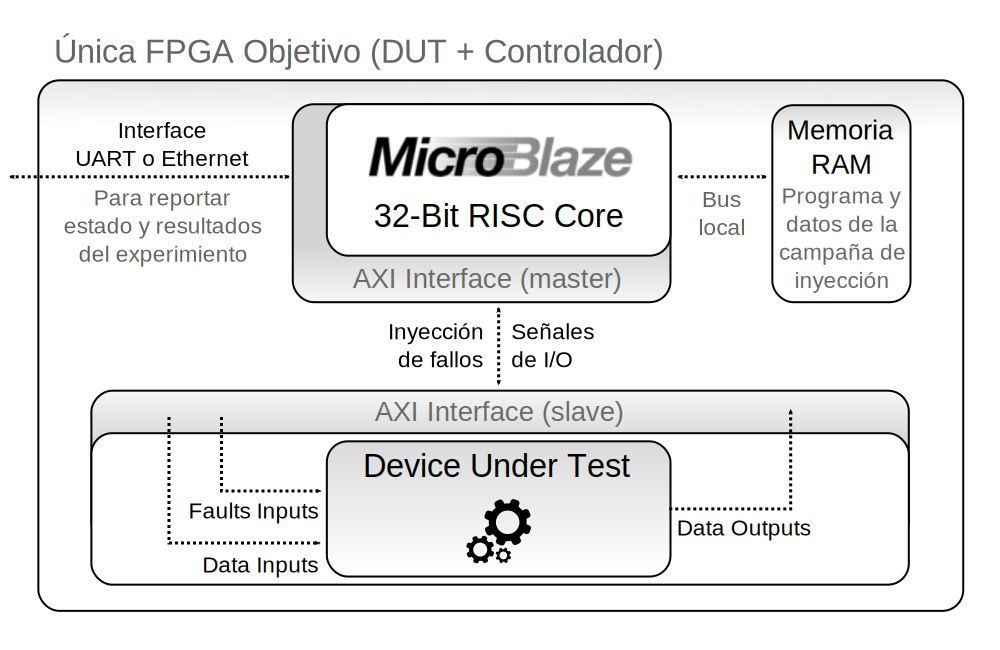
\includegraphics[width=0.75\textwidth]{img/netfi2.pdf}
	\caption{Diagrama en bloque de la arquitectura de NETFI-2}
	\label{netfi2}
\end{figure}

En la figura~\ref{netfi2} se muestra la arquitectura general de~\mbox{NETFI-2} integrada en una única FPGA donde se instancia el DUT y el controlador del experimento compuesto por el procesador de Xilinx. Este último hace uso de interfaces estándar como UART o Ethernet para comunicarse con el exterior y reportar el estado del experimento en curso o los resultados finales del mismo. Cabe destacar que el proceso de inyección de fallos no depende necesariamente de esta comunicación por lo que la velocidad de ejecución no se ve comprometida a diferencia de lo analizado en trabajos previos con controladores externos a la FPGA~\cite{Serrano2015}. Por el contrario, la campaña de inyección de fallos se puede ejecutar de manera autónoma dentro de la FPGA objetivo mientras se reportan los resultados parciales o totales a medida que el controlador dispone de margen de procesamiento.

% Procesador
El procesador MicroBlaze de Xilinx está basado en una arquitectura RISC de 32 bits que le permite tener una tasa aproximada de una instrucción por ciclo de reloj~\cite{uBlaze}. La arquitectura de este dispositivo puede personalizarse fácilmente  mediante las herramientas provistas por Xilinx. Para el acceso a la memoria de sistema, el procesador utiliza buses dedicados para instrucciones y datos lo que libera de carga a los demás buses. Esto es de particular importancia en NETFI-2 ya que permite contar con una interfaz basada en el protocolo AXI-Lite ~\cite{AXI} totalmente avocada a la ejecución del experimento de inyección y al reporte de su estado y resultado. 

\subsection{Experimento}

% Interface AXI
La interfaz AXI permite comunicar un dispositivo esclavo que contiene el experimento (DUT) con un maestro (procesador) que intercambian información entre ellos sin necesidad de utilizar demasiada área de la FPGA. Específicamente, el maestro utiliza mapeo de memoria para leer o escribir valores en registros de 32 bits (extensibles a 64) contenidos en el dispositivo esclavo como se ilustra en la figura~\ref{axi}. Según la especificación ofrecida por Xilinx, se pueden realizar hasta 256 transmisiones en ráfagas~\cite{AXI}. NETFI-2 utiliza este canal de comunicación tanto para configurar la inyección de fallos en los componentes ya intervenidos por MODNET (señales \emph{inject}) en el paso \circled{2} así como los valores de entrada y salida del DUT (señales \emph{input} y \emph{output}). Para ello, el dispositivo esclavo AXI mapea las direcciones de memoria del microprocesador con las señales del DUT bajo prueba.

\begin{figure}[H]
	\centering
	\includegraphics[width=0.75 \textwidth]{img/axi.pdf}
	\caption{Detalle de la comunicación con el DUT}
	\label{axi}
\end{figure}

\lstset{frame=tb,
  language=VHDL,
  aboveskip=3mm,
  belowskip=3mm,
  showstringspaces=false,
  columns=flexible,
  basicstyle=\ttfamily,
  numbers=none,
  breakatwhitespace=true,
  tabsize=2
}

\begin{figure}[H]
\centering
\begin{lstlisting}
entity AXI_Slave is 
	generic (
		C_S_AXI_DATA_WIDTH	: integer	:= 32; -- AXI data bus width
		C_S_AXI_ADDR_WIDTH	: integer	:= 32); -- AXI addr bus width
	port (...); -- AXI default ports
end AXI_Slave;

architecture AXI_Slave_imp of AXI_Slave is
	component DeviceUnder\textit{test} IS
		port (
			inject : IN  STD_LOGIC_VECTOR(81 DOWNTO 0);
			input : IN  STD_LOGIC_VECTOR(12 DOWNTO 0);
			output : OUT  STD_LOGIC
			clock : IN  STD_LOGIC; reset : IN  STD_LOGIC;);
	END component;
	signal  clock_to_dut   :  STD_LOGIC;
	signal  inject_to_dut   :  STD_LOGIC_VECTOR(81 DOWNTO 0);
	... 	-- Other AXI default signals
	begin
		... 	-- AXI default logic
		-- 81 bits for injection (82 fault points possible)
		inject_to_dut(31 downto 0) <= slv_reg5;
		inject_to_dut(63 downto 32) <= slv_reg6;
		inject_to_dut(81 downto 64) <= slv_reg7(17 downto 0);
		-- Enable DUT clock with bit 0 from slv_reg8
		clock_to_dut <= (S_AXI_ACLK and  slv_reg8(0)); 
		
		DeviceUnder\textit{test}_instance : DeviceUnder\textit{test}	
			port map (
				inject => inject_to_dut , input=>  slv_reg1(12 downto 0), 
				output => slv_reg4(0), clock => clock_to_dut, 
				reset => slv_reg0(0));			
end architecture AXI_Slave_imp of AXI_Slave
		
\end{lstlisting}
	\caption{Código VHDL del módulo AXI esclavo que contiene el DUT}
	\label{axi_slave}
\end{figure}

% AXI exclavo (Sophie)
Por otro lado, el Netlist del DUT modificado por MODNET se sintetiza en el formato EDIF para luego incluirse como componente del dispositivo AXI esclavo. Como se detalla en el código de la figura~\ref{axi_slave}, el componente $DeviceUnder\textit{test}$ cuenta con la cantidad de registros necesarios para recibir tanto la configuración de la inyección de fallos así como las entradas de del circuito bajo prueba. En general, la activación de fallos en el DUT modificado por MODNET se realiza por medio de un conjunto de banderas binarias $inject\_to\_dut$ cada una asociada a un punto posible de falla. Por ejemplo, el código de la figura~\ref{axi_slave} ilustra un total de 82 banderas con figuradas por 82 bits correspondientes a 3 registros esclavos ($slv\_reg5$, $slv\_reg6$ y $slv\_reg7$). Además de las señales de fallos, la arquitectura cuenta con una entrada $input$ de 13 bits, una salida $output$ de 1 bit y un control de \textit{clock} y \textit{reset} configurados en función del DUT a ensayar. Sin embargo, cabe destacar que la cantidad de registros y el mapeo específico a señales de fallos, entradas, o salidas  pueden adaptarse a las necesidades del DUT bajo prueba. 

\subsection{Programación}

La empresa Xilinx provee un entorno de desarrollo (SDK) específico para desarrollar software para el procesador Microblaze. Este software incluye las herramientas necesarias para facilitar la creación de código embebido con acceso a los perífericos del Microblaze por medio de \textit{drivers} y bibliotecas. Además, permite el despliegue del programa, su ejecución y su depuración. Dentro de los lenguajes permitidos se utilizó lenguaje C por su simplicidad y alto rendimiento. 

En la figura~\ref{c_example} se muestra un código ilustrativo que inyecta un fallo en la posición 4 y proporciona el resultado obtenido para la entrada $4095$ del DUT contenido en el AXI esclavo de la figura~\ref{axi_slave}. Esta pequeño programa se presenta como evidencia de la simplicidad con la que se puede diseñar campañas de inyección de fallos en el código del procesador Microblaze comunicado por una interfaz AXI. En efecto, el mismo programa puede determinar las salidas correctas sin fallos y luego compararlas con los resultados con fallos para finalmente determinar la sensibilidad del diseño bajo prueba.


\begin{figure}[H]
\centering
\begin{lstlisting}
#define AXI_BASEADDR 0x44A00000
int main(){
	int *baseaddr = AXI_BASEADDR;
	int *input = (baseaddr+1); //slv_reg1 (input in bit 0 to 12)
	int *output = (baseaddr+4); //slv_reg4 (output in bit 0)
	int *inject1 = (baseaddr+5); //slv_reg5 (fault in bit 0 to 31)
	int *inject2 = (baseaddr+6); //slv_reg6 (fault in bit 0 to 31)
	int *inject3 = (baseaddr+7); //slv_reg7 (fault in bit 0 to 17)
		
	*(input) = 4095; // 0xFFF (13its in input enabled)
	*(inject1) = 8; // 0X8 (fault in position 4) 
	*(inject2) = 0;
	*(inject3) = 0;
	// wait n clock cicles for DUT obtain the result
	printf("\%d\n",* (output));	
	return 0;}
\end{lstlisting}
	\caption{Código C para inyectar un fallo e imprimir el resultado del DUT}
	\label{c_example}
\end{figure}

En particular, y sobre todo con DUTs compuestos en su mayoría por lógica combinacional, es fundamental que el software sea capaz de inyectar fallos y leer la salida del circuito con la mínima cantidad de pulsos de reloj. Esto permite maximizar la cantidad de experimentos en un intervalo de tiempo dado. Sin embargo, es importante que el diseñador de la campaña contemple la cantidad de pulsos de reloj necesarios para que el DUT arroje la salida antes de leerla desde el código C. Por otro lado, cabe destacar que dado que los fallos se configuran por medio de banderas contenidas en registros, nada impide inyectar múltiples fallos (MBUs) al cambiar varias posiciones de los registros simultáneamente. Esto constituye una funcionalidad destacada de NETFI-2 en relación a los métodos ya existentes.

De esta manera, y retomando lo descrito en esta sección contextualizado en el flujo ilustrado en la figura~\ref{netfi_flow}, NETFI-2 extiende el paso~\circled{3} al incorporar en la síntesis el código del procesador Microblaze así como las interfaces y memorias asociadas. Luego, en el paso~\circled{4}, el experimento se puede realizar directamente sobre la FPGA destino sin necesidad de ningún hardware ni equipamiento extra.

\section{Evaluación y Validación}
\label{EvaluacionValidacion}

Para evaluar y validar NETFI-2 se propone un DUT ejemplo a modificar por MODNET para luego someterlo a la inyección de fallos tanto por medio de NETFI-2 así como por un método alternativo de simulación que servirá de patrón de referencia. Luego, además de comparar la igualdad de resultados, estudiaremos los tiempos requeridos por cada uno de estos métodos.

\subsection{Dispositivo Bajo Prueba}

Como DUT ejemplo, proponemos el uso de un módulo de una Máquina Bayesiana (BM) implementada en VHDL. Una BM es un tipo de computadora estocástica capaz de calcular inferencias Bayesianas basadas en un conjunto de distribuciones de probabilidad presentadas en su entrada~\cite{Mazer2015}. Estas máquinas basan su arquitectura interna en variables representadas como tren de bits estocásticos \textit{bitstreams} lo que las puede hacer relativamente resistentes a fallos. El lector interesado puede referirse a~\cite{Alaghi2013} para una revisión detallada de estos conceptos. En particular, una arquitectura de BM se sintetizo  en una FPGA y presentada en~\cite{Duarte2015}. 

En general, la BM propuesta se compone de pequeños módulos en paralelos denominados BM-Slice. Cada uno de estos toma como entrada 13 bits en representación del bus probabilístico y proporciona 1 bit de salida. En consecuencia, a mayor cantidad de BM-Slices, mayor la resolución de la salida estocástica del sistema. Además, la hipótesis sostenida en~\cite{Mazer2015} es que el sistema completo compuesto de $n$ BM-Slices debería ser intrínsicamente robusto ante fallos. En este primer trabajo evaluaremos la robustez de una BM-Slice individual con el fin de validar el método NETFI-2. Dejaremos como trabajo futuro y complementario estudiar la robustez de estas máquinas estocásticas de particular interés para algoritmos probabilísticos.

\subsection{Inyección de Fallos}

Para ejecutar la campaña de inyección de fallos se utilizaron los códigos VHDL de la BM-Slice para obtener el DUT a ensayar. Como se mostró en el paso~\circled{2} de la figura~\ref{netfi_flow}, los mismos se someten a MODNET para obtener los Netlist con los componentes sensibles a SET y SEU modificados. Para el caso de SET, MODNET detectó 82 puntos de fallos mientras que para SEU 27, lo que deriva en 82 y 27 bits de entrada al DUT modificado para activar estos fallos. Estos se agregan a los 13 bits de entrada del dato estocástico. La figura~\ref{axi_slave} ilustra el código VHDL que contiene el DUT modificado para inyección de SET. Luego, para los pasos~\circled{3} y \circled{4} se eligieron dos métodos diferentes: NETFI-2 e inyección por simulación. En efecto, este proceder permitirá contrastar y validar la eficacia de NETFI-2.

La campaña de inyección de fallos por emulación se realizó con NETFI-2 sobre una placa Nexys 4 equipada con una Xilinx Artix-7 XC7A100T-CS324. La síntesis del DUT modificado se realizó con la herramienta Synplify-Pro de Synopsys para obtener el archivo EDIF del mismo. Por otro lado, la síntesis del procesador y la generación del \textit{bitstream} de la FPGA se utilizó la herramienta Vivado de manera de dejar las herramientas preparadas para utilizar NETFI-2 con las FPGAs más modernas y económicas. Esto requirió de un trabajo adicional al reportado en~\cite{Mansour2013-1, Mansour2013-2} ya que las bibliotecas de Vivado difieren de las que venían en la anterior herramienta de Xilinx ISE. Cabe destacar que el procesador Microblaze embebido en esta plataforma fue configurado para trabajar con una frecuencia de 100 MHz.  

\renewcommand{\arraystretch}{1.2}
\begin{table}[H]
\centering
\caption{Detalle de Ocupación de Recursos en la FPGA Destino}
\label{Ocupacion}
\resizebox{0.45 \textwidth}{!}      \\ \hline
\multicolumn{1}{|l|}{Slice Registers} & \multicolumn{1}{c|}{1599}   & \multicolumn{1}{c|}{126800}      & \multicolumn{1}{c|}{1.26\%}      \\ \hline
                                      & \multicolumn{3}{c}{MicroBlaze + BM}                                                               \\ \hline \hline
\multicolumn{1}{|l|}{Slice LUTs}      & \multicolumn{1}{c|}{1687}   & \multicolumn{1}{c|}{63400}       & \multicolumn{1}{c|}{2.66\%}      \\ \hline
\multicolumn{1}{|l|}{Slice Registers} & \multicolumn{1}{c|}{1627}   & \multicolumn{1}{c|}{126800}      & \multicolumn{1}{c|}{1.28\%}      \\ \hline
                                      & \multicolumn{3}{c}{MicroBlaze + BM + Inyección SEU}                                               \\ \hline \hline
\multicolumn{1}{|l|}{Slice LUTs}      & \multicolumn{1}{c|}{1714}   & \multicolumn{1}{c|}{63400}       & \multicolumn{1}{c|}{2.70\%}      \\ \hline
\multicolumn{1}{|l|}{Slice Registers} & \multicolumn{1}{c|}{1627}   & \multicolumn{1}{c|}{126800}      & \multicolumn{1}{c|}{1.28\%}      \\ \hline
                                      & \multicolumn{3}{c}{MicroBlaze + BM + Inyección SET}                                               \\ \hline \hline
\multicolumn{1}{|l|}{Slice LUTs}      & \multicolumn{1}{c|}{1695}   & \multicolumn{1}{c|}{63400}       & \multicolumn{1}{c|}{2.67\%}      \\ \hline
\multicolumn{1}{|l|}{Slice Registers} & \multicolumn{1}{c|}{1629}   & \multicolumn{1}{c|}{126800}      & \multicolumn{1}{c|}{1.28\%}      \\ \hline
\end{tabular}%
}
\end{table}

La tabla ~\ref{Ocupacion} detalla los recursos requeridos para cada componente en la FPGA destino luego de realizar las modificaciones en las bibliotecas y actualizar la herramienta MODNET. En general, resulta interesante destacar que el procesador Microblaze (incluyendo la interfaz AXI) utilizado como controlador del experimento sólo requiere de un 2.53\% de LUTs y 1.26\% de registros de la FPGA destino. Si bien la BM-Slice bajo prueba es un circuito simple (i.e., sólo requiere de 80 LUTs y 28 registros), este análisis muestra que existe un margen de lugar suficiente para albergar DUTs de gran tamaño en NETFI-2. Por otro lado, se puede observar que MODNET incorpora 27 LUTs extras para el DUT modificado con los inyectores de SEU (se debe incorporar 1 multiplexor por cada FF sensible detectado), y 8 LUTs y 2 registros extras para los inyectores de SET (2 registros para las señales AXI necesarios para los 81 bits de inyección y 8 LUTs para extender los circuitos combinacionales sensibles). Esto quiere decir que el DUT extendido para inyección de SEU requiere de un 25\% de hardware adicional mientras que para la inyección de SET un 9.25\%.

Por otro lado, la inyección por simulación se realizó utilizando la herramienta ModelSim de Mentor Graphics~\cite{modelsim}. Dado que la simulación realizada es comportamental (i.e., no considera las demoras de propagación de las señales entre los módulos), la misma sólo resulta válida como patrón de referencia general y aproximada para los resultados físicos más realistas esperados en el hardware destino.

\subsection{Resultados}

Los resultados obtenidos de la inyección de fallos por simulación y emulación se resumen en la Tabla ~\ref{Resultados}. En general, las magnitudes obtenidas por ambas metodologías se corresponden validando la metodología NETFI-2 y evidenciando una susceptibilidad del circuito BM-Slice levemente superior al 10\% para SEU y 30\% para SET. En otras palabras, el circuito bajo prueba tiene algo más del 10\% y 30\% de posibilidades de proveer un resultado erróneo a la salida en caso de la presencia de un evento SEU o SET respectivamente. De acuerdo al conocimiento de los autores, este resultado es la primera evidencia respecto a la sensibilidad a la radiación del circuito bayesiano propuesto en~\cite{Duarte2015}.

\renewcommand{\arraystretch}{1.2}
\begin{table}[H]
\centering
\caption{Resultados de Inyección por Simulación y Emulación}
\label{Resultados}
\resizebox{0.47\textwidth}{!}{%
\begin{tabular}{l|c|c|}
\cline{2-3}
& \begin{tabular}[c]{@{}c@{}}Tasa de Errores\\ SEU\end{tabular} & \begin{tabular}[c]{@{}c@{}}Tasa de Errores\\ SET\end{tabular} \\ \hline \hline
\multicolumn{1}{|l|}{Simulación (ModelSim)} & 13.69\%                                                       & 31.77\%                                                       \\ \hline
\multicolumn{1}{|l|}{Emulación (NETFI-2)}   & 11.90\%                                                       & 32.77\%                                                       \\ \hline
\end{tabular}%
}
\end{table}



\begin{table}[H]
\centering
\caption{Tiempos de Ejecución de Inyección por Simulación y Emulación}
\label{ResultadosTiempo}
\resizebox{0.46\textwidth}{!}{%
\begin{tabular}{l|c|c|}
\cline{2-3}
                                            & \begin{tabular}[c]{@{}c@{}}Tiempo de\\ Ejecución SEU\end{tabular} & \begin{tabular}[c]{@{}c@{}}Tiempo de\\ Ejecución SET\end{tabular} \\ \hline \hline
\multicolumn{1}{|l|}{Simulación (ModelSim)} & 269 s                                                             & 327 s                                                             \\ \hline
\multicolumn{1}{|l|}{Emulación (NETFI-2)}   & \textless 1 s                                                  & \textless 1 s                                                  \\ \hline
\end{tabular}%
}
\end{table}

Por otro lado, resulta de interés medir los tiempos de ejecución involucrados en cada una de estas metodologías. La tabla ~\ref{ResultadosTiempo} detalla las mediciones realizadas para las inyecciones en el circuito BM-Slice. De acuerdo a lo ya descrito para las metodologías de simulación y emulación, las primeras requieren de un considerable esfuerzo computacional inclusive para circuitos sencillos como el caso de BM-Slice. En efecto, a mayor el tamaño del DUT, mayor relevancia toman las metodologías de emulación como NETFI-2, que para este caso particular permite realizar la campaña de inyección exhaustiva en menos de un segundo (i.e., aproximadamente 300\% más rápido).

\section{Resumen}
\label{Conclusion}

En este capítulo se presentó la problemática de la inyección de fallos en circuitos integrados con el fin de evaluar su sensibilidad a las alteraciones provocadas por eventos de radiación cada vez más frecuentes debido a creciente escala de integración. En particular, se retomó un trabajo previo de inyección por emulación para extenderlo, actualizarlo, y mejorarlo. Bajo el nombre de NETFI-2, se describió en detalle el flujo de trabajo de esta nueva metodología resaltando sus ventajas respecto a aportes anteriores.

Con el fin de validar y mensurar el comportamiento de NETFI-2, se propuso un caso de uso práctico de un circuito que implementa una Máquina Bayesiana. Por un lado, este experimento arrojó los primeros resultados de un circuito de este tipo, y por otro, permitió contrastar los resultados de NETFI-2 con metodologías de simulación semejantes. En efecto, se verificó que el método arroja resultados coherentes con los obtenidos por simulación mejorando en más de un 300\% la velocidad de ejecución. Además, los resultados de NETFI-2 se consideran de mayor realismo dado que los mismos modelan efectos físicos como las demoras de propagación no consideradas por simulaciones comportamentales. Finalmente, se analizó la ocupación de FPGA requerida por el controlador NETFI-2 mostrando que el mismo sólo requiere de una pequeña área del dispositivo destino.




\makeatletter
\@addtoreset{chapter}{part}
\makeatother
\chapter{Conclusión y trabajos futuros}

\section{Conclusión }
Entre  los diferentes  enfoques para determinar si un circuito es robusto frente a los efectos de la radiación, particularmente los SEEs, la emulación de fallos es uno de los más pertinentes por costos y requerimientos.


Este trabajo propone una herramienta y un  método, el cual se puede apreciar en la figura \ref{proceso3}, que posee varias ventajas entre las que  se pueden mencionar: 
\begin{itemize}
\item Esfuerzo reducido para realizar una campaña de inyeccion de fallas sobre el DUT.
\item Tiempo requerido para obtener resultados, inferior a los tiempos requeridos por una simulación.
\item  Utilización del lenguaje C, ampliamente conocido, para programar  una campaña de inyección de fallas sobre un RTL.

\item Esto último representa una ventaja frente a otros métodos al partir de un código de bajo nivel en VHDL o Verilog y generar una capa de abstracción en un lenguaje de alto nivel. 

\item Reducido espacio de memoria para instanciar el controlador sobre la FPGA.

\item Reproducible y escalable para todas las FPGAs a partir de la generación 7-series.
\end{itemize}




  \section{Debilidades }
Por otra parte tiene aspectos y puntos a mejorar, entre los que  se pueden citar:

\begin{itemize}
\item Extra hardware generado  por la herramienta MODNET comparable al tamaño del circuito que se desea probar y proporcional a su lógica.
\item La comunicación vía UART es lenta y demora las campañas.
\item Es complicado estimar los tiempos de una campaña si se estiman a partir del lenguaje de alto nivel.

\end{itemize}



\begin{figure}[H]
	\centering
	\includegraphics[width=0.75\textwidth]{img/Abstraccion.pdf}
	\caption{Descripción de NetFi2 }
	\label{proceso3}
    \end{figure}



\section{Mejoras y Trabajos futuros }


Entre las mejoras a realizar, queda por encontrar un método factible que permita cuantificar en proporciones, la cantidad de hardware extra en función al circuito a someter.
Existen alternativas como la nueva generación de las bibliotecas de Xilinx, las cuales son más genéricas y podrían disminuir la cantidad de extra hardware y  a través de ellas hasta predecir la proporción  que será necesaria agregar.

Respecto a la interface de comunicación, la mayoría de las FPGAs actualmente cuentan con el puerto Ethernet.  Instanciarlo tendría una doble funcionalidad en el método, primero permitiría tener un taza de transferencia  de datos por unidad de tiempo muy superior al conseguido por la UART y en segundo lugar se generaría la posibilidad de realizar campañas de inyección de forma remota.

Por otro lado, para campañas en las cuales las inyecciones se realizan en ventanas de tiempo, es posible realizarlas utilizando el TIMER y las funciones de tiempo en C. Sin embargo, queda por profundizar qué tan preciso es y sobre todo qué posibilidades habría de hacerlo funcionar al TIMER como generador de ciclos de reloj dedicado, por ejemplo para  casos en que se hagan campañas sobre microprocesadores como el LEON3. 

Otra posible aplicación  para NetFi2,  si se tuviese el \textit{layout} del circuito a someter, podría ser realizar campañas de inyecciones múltiples, emulando MBUs y MCUs.


Finalmente, se desearía que todo el método fuese automático. Esto sería posible si se utilizan los escripts en TCL, lo cuales permitirían realizar todo una campaña de forma automática, siguiendo algunos pocos parámetros de entrada designados por el usuario.





Como trabajos futuros se propone integrar el flujo de trabajo completo de NETFI-2 en una única herramienta de software que permita automatizar todo el proceso incluyendo la posibilidad de realizar experimentos bajo radiación. Por otro lado, resulta de interés explorar la posibilidad de trasladar el controlador embebido en la FPGA a otros procesadores ya incluidos en algunas de estas plataformas (generalmente de arquitectura ARM) para liberar espacio.


El LCSR  tiene previsto llevar adelante la fusión entre \textit{Fault Tolerance} y \textit{Delay Tolerant Networks} (DTN), entre otras líneas de investigación que requieren como base disponer de un inyector de fallas en tiempo real. De hecho, la fusión entre este emulador de fallas y un simulador de redes DTN, será una de las principales tareas a desarrollar por el LCSR en el futuro próximo

Para concluir, los próximos pasos que se planean ejecutar involucran la generación de un DUT del procesador LEON-3 para evaluar la robustez de aplicaciones bajo entornos susceptibles a fallas por radiación.

    
\bibliographystyle{unsrt}


\bibliography{bibfile}
Toda la bibliográfica consultada en sitios webs corresponde a consultas realizadas entre los meses Marzo y Octubre del año 2016. 
\appendix
\chapter{Bibliotecas originales y modificadas }\label{aped.A}

\section{FDC}
\begin{lstlisting}

module FDC (Q, C, CLR, D);

    parameter INIT = 1'b0;

    output Q;

    input  C, CLR, D;

    wire Q;
    reg q_out;
    tri0 GSR = glbl.GSR;

    initial q_out = INIT;


    always @(GSR or CLR)
      if (GSR)
            assign q_out = INIT;
      else if (CLR)
           assign q_out = 0;
      else
            deassign q_out;

    always @(posedge C)
	         q_out <=  D;

    assign Q = q_out;

    specify
        (posedge CLR => (Q +: 1'b0)) = (0, 0);
        if (!CLR)
            (posedge C => (Q +: D)) = (100, 100);
    endspecify
endmodule
\end{lstlisting}

\section{FDC\_MOD}
\begin{lstlisting}


`timescale  1 ps / 1 ps

module FDC_mod (inj, Q, C, CLR, D);

parameter INIT = 1'b0;

output Q;

input C, CLR, D, inj;

wire Din;

FDC uut_FDC(.Q(Q),.C(C),.CLR(CLR),.D(Din));

assign Din = (inj) ? !D : D;

endmodule

\end{lstlisting}


\section{LUT4}
\begin{lstlisting}


module LUT4 (O, I0, I1, I2, I3);

  parameter INIT = 16'h0000;

  input I0, I1, I2, I3;

  output O;

  reg O;
  reg tmp;

  always @( I3 or  I2 or  I1 or  I0)  begin
 
    tmp =  I0 ^ I1  ^ I2 ^ I3;

    if (tmp == 0 || tmp == 1)

        O = INIT[{I3, I2, I1, I0}];

    else 
    
      O =  lut4_mux4 ({lut4_mux4 (INIT[15:12], {I1, I0}),
                          lut4_mux4 (INIT[11:8], {I1, I0}),
                          lut4_mux4 (INIT[7:4], {I1, I0}),
                          lut4_mux4 (INIT[3:0], {I1, I0}) }, {I3, I2});
  end

  function lut4_mux4;
  input [3:0] d;
  input [1:0] s;
   
  begin

       if ((s[1]^s[0] ==1) || (s[1]^s[0] ==0))
           
           lut4_mux4 = d[s];

         else if ((d[0] === d[1]) && (d[2] === d[3]) && (d[0] === d[2])) 
           lut4_mux4 = d[0];
         else if ((s[1] == 0) && (d[0] === d[1]))
           lut4_mux4 = d[0];
         else if ((s[1] == 1) && (d[2] === d[3])) 
           lut4_mux4 = d[2];
         else if ((s[0] == 0) && (d[0] === d[2])) 
           lut4_mux4 = d[0];
         else if ((s[0] == 1) && (d[1] === d[3]))
           lut4_mux4 = d[1];
         else
           lut4_mux4 = 1'bx;
   end
  endfunction

endmodule

\end{lstlisting}

\section{LUT4\_MOD}
\begin{lstlisting}

module LUT4_mod (inj_c, O, I0, I1, I2, I3);

  parameter INIT = 16'h0000;

  input inj_c, I0, I1, I2, I3;

  output O;

  reg O1;
  reg tmp;

  
    assign O = (!inj_c) ? O1 : !O1 ;
	
	
  always @( I3 or  I2 or  I1 or  I0)  begin
 
    tmp =  I0 ^ I1  ^ I2 ^ I3;

    if (tmp == 0 || tmp == 1)

        O1 = INIT[{I3, I2, I1, I0}];

    else 
    
      O1 =  lut4_mux4 ({lut4_mux4 (INIT[15:12], {I1, I0}),
                          lut4_mux4 (INIT[11:8], {I1, I0}),
                          lut4_mux4 (INIT[7:4], {I1, I0}),
                          lut4_mux4 (INIT[3:0], {I1, I0}) }, {I3, I2});
  end

  function lut4_mux4;
  input [3:0] d;
  input [1:0] s;
   
  begin

       if ((s[1]^s[0] ==1) || (s[1]^s[0] ==0))
           
           lut4_mux4 = d[s];

         else if ((d[0] === d[1]) && (d[2] === d[3]) && (d[0] === d[2])) 
           lut4_mux4 = d[0];
         else if ((s[1] == 0) && (d[0] === d[1]))
           lut4_mux4 = d[0];
         else if ((s[1] == 1) && (d[2] === d[3])) 
           lut4_mux4 = d[2];
         else if ((s[0] == 0) && (d[0] === d[2])) 
           lut4_mux4 = d[0];
         else if ((s[0] == 1) && (d[1] === d[3]))
           lut4_mux4 = d[1];
         else
           lut4_mux4 = 1'bx;
   end
  endfunction

endmodule


\end{lstlisting}

\section{LUT4\_L}
\begin{lstlisting}
module LUT4_L (LO, I0, I1, I2, I3);

  parameter INIT = 16'h0000;

  input inj_c, I0, I1, I2, I3;

  output LO;

  reg LO;
  reg tmp;

  
 
  

  
  always @( I3 or  I2 or  I1 or  I0)  begin
 
    tmp =  I0 ^ I1  ^ I2 ^ I3;

    if (tmp == 0 || tmp == 1)

        LO = INIT[{I3, I2, I1, I0}];

    else 
    
      LO =  lut4_mux4 ({lut4_mux4 (INIT[15:12], {I1, I0}),
                          lut4_mux4 (INIT[11:8], {I1, I0}),
                          lut4_mux4 (INIT[7:4], {I1, I0}),
                          lut4_mux4 (INIT[3:0], {I1, I0}) }, {I3, I2});
  end

  function lut4_mux4;
  input [3:0] d;
  input [1:0] s;
   
  begin

       if ((s[1]^s[0] ==1) || (s[1]^s[0] ==0))
           
           lut4_mux4 = d[s];

         else if ((d[0] === d[1]) && (d[2] === d[3]) && (d[0] === d[2])) 
           lut4_mux4 = d[0];
         else if ((s[1] == 0) && (d[0] === d[1]))
           lut4_mux4 = d[0];
         else if ((s[1] == 1) && (d[2] === d[3])) 
           lut4_mux4 = d[2];
         else if ((s[0] == 0) && (d[0] === d[2])) 
           lut4_mux4 = d[0];
         else if ((s[0] == 1) && (d[1] === d[3]))
           lut4_mux4 = d[1];
         else
           lut4_mux4 = 1'bx;
   end
  endfunction

endmodule


\end{lstlisting}

\section{LUT4\_L\_mod}
\begin{lstlisting}
module LUT4_L_mod (inj_c, LO, I0, I1, I2, I3);

  parameter INIT = 16'h0000;

  input inj_c, I0, I1, I2, I3;

  output LO;

  reg LO1;
  reg tmp;

  
  assign LO = (!inj_c) ? LO1 : !LO1;
  
  always @( I3 or  I2 or  I1 or  I0)  begin
 
    tmp =  I0 ^ I1  ^ I2 ^ I3;

    if (tmp == 0 || tmp == 1)

        LO1 = INIT[{I3, I2, I1, I0}];

    else 
    
      LO1 =  lut4_mux4 ({lut4_mux4 (INIT[15:12], {I1, I0}),
                          lut4_mux4 (INIT[11:8], {I1, I0}),
                          lut4_mux4 (INIT[7:4], {I1, I0}),
                          lut4_mux4 (INIT[3:0], {I1, I0}) }, {I3, I2});
  end

  function lut4_mux4;
  input [3:0] d;
  input [1:0] s;
   
  begin

       if ((s[1]^s[0] ==1) || (s[1]^s[0] ==0))
           
           lut4_mux4 = d[s];

         else if ((d[0] === d[1]) && (d[2] === d[3]) && (d[0] === d[2])) 
           lut4_mux4 = d[0];
         else if ((s[1] == 0) && (d[0] === d[1]))
           lut4_mux4 = d[0];
         else if ((s[1] == 1) && (d[2] === d[3])) 
           lut4_mux4 = d[2];
         else if ((s[0] == 0) && (d[0] === d[2])) 
           lut4_mux4 = d[0];
         else if ((s[0] == 1) && (d[1] === d[3]))
           lut4_mux4 = d[1];
         else
           lut4_mux4 = 1'bx;
   end
  endfunction

endmodule
\end{lstlisting}

\section{LUT5}
\begin{lstlisting}

module LUT5 (O, I0, I1, I2, I3, I4);

  parameter INIT = 32'h00000000;

  input I0, I1, I2, I3, I4;

  output O;

  reg O;
  reg tmp;

  always @(I4 or I3 or  I2 or  I1 or  I0)  begin
 
    tmp =  I0 ^ I1  ^ I2 ^ I3 ^ I4;

    if (tmp == 0 || tmp == 1)

        O = INIT[{I4, I3, I2, I1, I0}];

    else 
    
      O =  lut4_mux4 (
                        { lut6_mux8 (INIT[31:24], {I2, I1, I0}),
                          lut6_mux8 (INIT[23:16], {I2, I1, I0}),
                          lut6_mux8 (INIT[15:8], {I2, I1, I0}),
                          lut6_mux8 (INIT[7:0], {I2, I1, I0}) }, { I4, I3});
  end

  function lut6_mux8;
  input [7:0] d;
  input [2:0] s;
   
  begin

       if ((s[2]^s[1]^s[0] ==1) || (s[2]^s[1]^s[0] ==0))
           
           lut6_mux8 = d[s];

         else
           if (~(|d))
                 lut6_mux8 = 1'b0;
           else if ((&d))
                 lut6_mux8 = 1'b1;
           else if (((s[1]^s[0] ==1'b1) || (s[1]^s[0] ==1'b0)) &&
           (d[{1'b0,s[1:0]}]===d[{1'b1,s[1:0]}]))
                 lut6_mux8 = d[{1'b0,s[1:0]}];
           else if (((s[2]^s[0] ==1) || (s[2]^s[0] ==0)) && 
           (d[{s[2],1'b0,s[0]}]===d[{s[2],1'b1,s[0]}]))
                 lut6_mux8 = d[{s[2],1'b0,s[0]}];
           else if (((s[2]^s[1] ==1) || (s[2]^s[1] ==0)) && 
           (d[{s[2],s[1],1'b0}]===d[{s[2],s[1],1'b1}]))
                 lut6_mux8 = d[{s[2],s[1],1'b0}];
           else if (((s[0] ==1) || (s[0] ==0)) &&
           (d[{1'b0,1'b0,s[0]}]===d[{1'b0,1'b1,s[0]}]) &&
              (d[{1'b0,1'b0,s[0]}]===d[{1'b1,1'b0,s[0]}]) && 
              (d[{1'b0,1'b0,s[0]}]===d[{1'b1,1'b1,s[0]}]))
                 lut6_mux8 = d[{1'b0,1'b0,s[0]}];
           else if (((s[1] ==1) || (s[1] ==0)) &&
           (d[{1'b0,s[1],1'b0}]===d[{1'b0,s[1],1'b1}]) &&
              (d[{1'b0,s[1],1'b0}]===d[{1'b1,s[1],1'b0}]) && 
              (d[{1'b0,s[1],1'b0}]===d[{1'b1,s[1],1'b1}]))
                 lut6_mux8 = d[{1'b0,s[1],1'b0}];
           else if (((s[2] ==1) || (s[2] ==0)) && 
           (d[{s[2],1'b0,1'b0}]===d[{s[2],1'b0,1'b1}]) &&
              (d[{s[2],1'b0,1'b0}]===d[{s[2],1'b1,1'b0}]) && 
              (d[{s[2],1'b0,1'b0}]===d[{s[2],1'b1,1'b1}]))
                 lut6_mux8 = d[{s[2],1'b0,1'b0}];
           else
                 lut6_mux8 = 1'bx;
   end
  endfunction


  function lut4_mux4;
  input [3:0] d;
  input [1:0] s;
   
  begin

       if ((s[1]^s[0] ==1) || (s[1]^s[0] ==0))

           lut4_mux4 = d[s];

         else if ((d[0] === d[1]) && (d[2] === d[3])  && (d[0] === d[2]))
           lut4_mux4 = d[0];
         else if ((s[1] == 0) && (d[0] === d[1]))
           lut4_mux4 = d[0];
         else if ((s[1] == 1) && (d[2] === d[3]))
           lut4_mux4 = d[2];
         else if ((s[0] == 0) && (d[0] === d[2]))
           lut4_mux4 = d[0];
         else if ((s[0] == 1) && (d[1] === d[3]))
           lut4_mux4 = d[1];
         else
           lut4_mux4 = 1'bx;

   end
  endfunction

endmodule
\end{lstlisting}

\section{LUT5\_MOD}
\begin{lstlisting}
module LUT5_mod (inj_c,O1, I0, I1, I2, I3, I4);

  parameter INIT = 32'h00000000;

  input inj_c, I0, I1, I2, I3, I4;

  output O;

  reg O1;
  reg tmp;
  
  assign O = (!inj_c) ? O1 : !O1;

  always @(I4 or I3 or  I2 or  I1 or  I0)  begin
 
    tmp =  I0 ^ I1  ^ I2 ^ I3 ^ I4;

    if (tmp == 0 || tmp == 1)

        O1 = INIT[{I4, I3, I2, I1, I0}];

    else 
    
      O1 =  lut4_mux4 (
                        { lut6_mux8 (INIT[31:24], {I2, I1, I0}),
                          lut6_mux8 (INIT[23:16], {I2, I1, I0}),
                          lut6_mux8 (INIT[15:8], {I2, I1, I0}),
                          lut6_mux8 (INIT[7:0], {I2, I1, I0}) }, { I4, I3});
  end

  function lut6_mux8;
  input [7:0] d;
  input [2:0] s;
   
  begin

       if ((s[2]^s[1]^s[0] ==1) || (s[2]^s[1]^s[0] ==0))
           
           lut6_mux8 = d[s];

         else
           if (~(|d))
                 lut6_mux8 = 1'b0;
           else if ((&d))
                 lut6_mux8 = 1'b1;
           else if (((s[1]^s[0] ==1'b1) || (s[1]^s[0] ==1'b0)) &&
           (d[{1'b0,s[1:0]}]===d[{1'b1,s[1:0]}]))
                 lut6_mux8 = d[{1'b0,s[1:0]}];
           else if (((s[2]^s[0] ==1) || (s[2]^s[0] ==0)) && 
           (d[{s[2],1'b0,s[0]}]===d[{s[2],1'b1,s[0]}]))
                 lut6_mux8 = d[{s[2],1'b0,s[0]}];
           else if (((s[2]^s[1] ==1) || (s[2]^s[1] ==0)) && 
           (d[{s[2],s[1],1'b0}]===d[{s[2],s[1],1'b1}]))
                 lut6_mux8 = d[{s[2],s[1],1'b0}];
           else if (((s[0] ==1) || (s[0] ==0)) && 
           (d[{1'b0,1'b0,s[0]}]===d[{1'b0,1'b1,s[0]}]) &&
              (d[{1'b0,1'b0,s[0]}]===d[{1'b1,1'b0,s[0]}]) && 
              (d[{1'b0,1'b0,s[0]}]===d[{1'b1,1'b1,s[0]}]))
                 lut6_mux8 = d[{1'b0,1'b0,s[0]}];
           else if (((s[1] ==1) || (s[1] ==0)) && 
           (d[{1'b0,s[1],1'b0}]===d[{1'b0,s[1],1'b1}]) &&
              (d[{1'b0,s[1],1'b0}]===d[{1'b1,s[1],1'b0}]) && 
              (d[{1'b0,s[1],1'b0}]===d[{1'b1,s[1],1'b1}]))
                 lut6_mux8 = d[{1'b0,s[1],1'b0}];
           else if (((s[2] ==1) || (s[2] ==0)) &&
           (d[{s[2],1'b0,1'b0}]===d[{s[2],1'b0,1'b1}]) &&
              (d[{s[2],1'b0,1'b0}]===d[{s[2],1'b1,1'b0}]) &&
              (d[{s[2],1'b0,1'b0}]===d[{s[2],1'b1,1'b1}]))
                 lut6_mux8 = d[{s[2],1'b0,1'b0}];
           else
                 lut6_mux8 = 1'bx;
   end
  endfunction


  function lut4_mux4;
  input [3:0] d;
  input [1:0] s;
   
  begin

       if ((s[1]^s[0] ==1) || (s[1]^s[0] ==0))

           lut4_mux4 = d[s];

         else if ((d[0] === d[1]) && (d[2] === d[3])  && (d[0] === d[2]))
           lut4_mux4 = d[0];
         else if ((s[1] == 0) && (d[0] === d[1]))
           lut4_mux4 = d[0];
         else if ((s[1] == 1) && (d[2] === d[3]))
           lut4_mux4 = d[2];
         else if ((s[0] == 0) && (d[0] === d[2]))
           lut4_mux4 = d[0];
         else if ((s[0] == 1) && (d[1] === d[3]))
           lut4_mux4 = d[1];
         else
           lut4_mux4 = 1'bx;

   end
  endfunction

endmodule
\end{lstlisting}

\section{LUT5\_L}
\begin{lstlisting}
module LUT5_L (LO, I0, I1, I2, I3, I4);

  parameter INIT = 32'h00000000;

  input inj_c,I0, I1, I2, I3, I4;

  output LO;

  reg LO;
  reg tmp;
  
  

  always @(I4 or I3 or  I2 or  I1 or  I0)  begin
 
    tmp =  I0 ^ I1  ^ I2 ^ I3 ^ I4;

    if (tmp == 0 || tmp == 1)

        LO1 = INIT[{I4, I3, I2, I1, I0}];

    else 
    
      LO1 =  lut4_mux4 (
                        { lut6_mux8 (INIT[31:24], {I2, I1, I0}),
                          lut6_mux8 (INIT[23:16], {I2, I1, I0}),
                          lut6_mux8 (INIT[15:8], {I2, I1, I0}),
                          lut6_mux8 (INIT[7:0], {I2, I1, I0}) }, { I4, I3});
  end

  function lut6_mux8;
  input [7:0] d;
  input [2:0] s;
   
  begin

       if ((s[2]^s[1]^s[0] ==1) || (s[2]^s[1]^s[0] ==0))
           
           lut6_mux8 = d[s];

         else
           if (~(|d))
                 lut6_mux8 = 1'b0;
           else if ((&d))
                 lut6_mux8 = 1'b1;
           else if (((s[1]^s[0] ==1'b1) || (s[1]^s[0] ==1'b0)) &&
           (d[{1'b0,s[1:0]}]===d[{1'b1,s[1:0]}]))
                 lut6_mux8 = d[{1'b0,s[1:0]}];
           else if (((s[2]^s[0] ==1) || (s[2]^s[0] ==0)) &&
           (d[{s[2],1'b0,s[0]}]===d[{s[2],1'b1,s[0]}]))
                 lut6_mux8 = d[{s[2],1'b0,s[0]}];
           else if (((s[2]^s[1] ==1) || (s[2]^s[1] ==0)) && 
           (d[{s[2],s[1],1'b0}]===d[{s[2],s[1],1'b1}]))
                 lut6_mux8 = d[{s[2],s[1],1'b0}];
           else if (((s[0] ==1) || (s[0] ==0)) && 
           (d[{1'b0,1'b0,s[0]}]===d[{1'b0,1'b1,s[0]}]) &&
              (d[{1'b0,1'b0,s[0]}]===d[{1'b1,1'b0,s[0]}]) &&
              (d[{1'b0,1'b0,s[0]}]===d[{1'b1,1'b1,s[0]}]))
                 lut6_mux8 = d[{1'b0,1'b0,s[0]}];
           else if (((s[1] ==1) || (s[1] ==0)) && 
           (d[{1'b0,s[1],1'b0}]===d[{1'b0,s[1],1'b1}]) &&
              (d[{1'b0,s[1],1'b0}]===d[{1'b1,s[1],1'b0}]) && 
              (d[{1'b0,s[1],1'b0}]===d[{1'b1,s[1],1'b1}]))
                 lut6_mux8 = d[{1'b0,s[1],1'b0}];
           else if (((s[2] ==1) || (s[2] ==0)) && 
           (d[{s[2],1'b0,1'b0}]===d[{s[2],1'b0,1'b1}]) &&
              (d[{s[2],1'b0,1'b0}]===d[{s[2],1'b1,1'b0}]) &&
              (d[{s[2],1'b0,1'b0}]===d[{s[2],1'b1,1'b1}]))
                 lut6_mux8 = d[{s[2],1'b0,1'b0}];
           else
                 lut6_mux8 = 1'bx;
   end
  endfunction


  function lut4_mux4;
  input [3:0] d;
  input [1:0] s;
   
  begin

       if ((s[1]^s[0] ==1) || (s[1]^s[0] ==0))

           lut4_mux4 = d[s];

         else if ((d[0] === d[1]) && (d[2] === d[3])  && (d[0] === d[2]))
           lut4_mux4 = d[0];
         else if ((s[1] == 0) && (d[0] === d[1]))
           lut4_mux4 = d[0];
         else if ((s[1] == 1) && (d[2] === d[3]))
           lut4_mux4 = d[2];
         else if ((s[0] == 0) && (d[0] === d[2]))
           lut4_mux4 = d[0];
         else if ((s[0] == 1) && (d[1] === d[3]))
           lut4_mux4 = d[1];
         else
           lut4_mux4 = 1'bx;

   end
  endfunction

endmodule
\end{lstlisting}

\section{LUT5\_L\_MOD}
\begin{lstlisting}
module LUT5_L_mod (inj_c,LO, I0, I1, I2, I3, I4);

  parameter INIT = 32'h00000000;

  input inj_c,I0, I1, I2, I3, I4;

  output LO;

  reg LO1;
  reg tmp;
  
   assign LO = (!inj_c) ? LO1 : !LO1;

  always @(I4 or I3 or  I2 or  I1 or  I0)  begin
 
    tmp =  I0 ^ I1  ^ I2 ^ I3 ^ I4;

    if (tmp == 0 || tmp == 1)

        LO1 = INIT[{I4, I3, I2, I1, I0}];

    else 
    
      LO1 =  lut4_mux4 (
                        { lut6_mux8 (INIT[31:24], {I2, I1, I0}),
                          lut6_mux8 (INIT[23:16], {I2, I1, I0}),
                          lut6_mux8 (INIT[15:8], {I2, I1, I0}),
                          lut6_mux8 (INIT[7:0], {I2, I1, I0}) }, { I4, I3});
  end

  function lut6_mux8;
  input [7:0] d;
  input [2:0] s;
   
  begin

       if ((s[2]^s[1]^s[0] ==1) || (s[2]^s[1]^s[0] ==0))
           
           lut6_mux8 = d[s];

         else
           if (~(|d))
                 lut6_mux8 = 1'b0;
           else if ((&d))
                 lut6_mux8 = 1'b1;
           else if (((s[1]^s[0] ==1'b1) || (s[1]^s[0] ==1'b0)) &&
           (d[{1'b0,s[1:0]}]===d[{1'b1,s[1:0]}]))
                 lut6_mux8 = d[{1'b0,s[1:0]}];
           else if (((s[2]^s[0] ==1) || (s[2]^s[0] ==0)) && 
           (d[{s[2],1'b0,s[0]}]===d[{s[2],1'b1,s[0]}]))
                 lut6_mux8 = d[{s[2],1'b0,s[0]}];
           else if (((s[2]^s[1] ==1) || (s[2]^s[1] ==0)) && 
           (d[{s[2],s[1],1'b0}]===d[{s[2],s[1],1'b1}]))
                 lut6_mux8 = d[{s[2],s[1],1'b0}];
           else if (((s[0] ==1) || (s[0] ==0)) &&
           (d[{1'b0,1'b0,s[0]}]===d[{1'b0,1'b1,s[0]}]) &&
              (d[{1'b0,1'b0,s[0]}]===d[{1'b1,1'b0,s[0]}]) && 
              (d[{1'b0,1'b0,s[0]}]===d[{1'b1,1'b1,s[0]}]))
                 lut6_mux8 = d[{1'b0,1'b0,s[0]}];
           else if (((s[1] ==1) || (s[1] ==0)) &&
           (d[{1'b0,s[1],1'b0}]===d[{1'b0,s[1],1'b1}]) &&
              (d[{1'b0,s[1],1'b0}]===d[{1'b1,s[1],1'b0}]) &&
              (d[{1'b0,s[1],1'b0}]===d[{1'b1,s[1],1'b1}]))
                 lut6_mux8 = d[{1'b0,s[1],1'b0}];
           else if (((s[2] ==1) || (s[2] ==0)) && 
           (d[{s[2],1'b0,1'b0}]===d[{s[2],1'b0,1'b1}]) &&
              (d[{s[2],1'b0,1'b0}]===d[{s[2],1'b1,1'b0}]) &&
              (d[{s[2],1'b0,1'b0}]===d[{s[2],1'b1,1'b1}]))
                 lut6_mux8 = d[{s[2],1'b0,1'b0}];
           else
                 lut6_mux8 = 1'bx;
   end
  endfunction


  function lut4_mux4;
  input [3:0] d;
  input [1:0] s;
   
  begin

       if ((s[1]^s[0] ==1) || (s[1]^s[0] ==0))

           lut4_mux4 = d[s];

         else if ((d[0] === d[1]) && (d[2] === d[3])  && (d[0] === d[2]))
           lut4_mux4 = d[0];
         else if ((s[1] == 0) && (d[0] === d[1]))
           lut4_mux4 = d[0];
         else if ((s[1] == 1) && (d[2] === d[3]))
           lut4_mux4 = d[2];
         else if ((s[0] == 0) && (d[0] === d[2]))
           lut4_mux4 = d[0];
         else if ((s[0] == 1) && (d[1] === d[3]))
           lut4_mux4 = d[1];
         else
           lut4_mux4 = 1'bx;

   end
  endfunction

endmodule

\end{lstlisting}

\section{LUT6}
\begin{lstlisting}
module LUT6 (O, I0, I1, I2, I3, I4, I5);

  parameter INIT = 64'h0000000000000000;

  input I0, I1, I2, I3, I4, I5;

  output O;

  reg O;
  reg tmp;

  always @(I5 or I4 or I3 or  I2 or  I1 or  I0)  begin
 
    tmp =  I0 ^ I1  ^ I2 ^ I3 ^ I4 ^ I5;

    if (tmp == 0 || tmp == 1)

        O = INIT[{I5, I4, I3, I2, I1, I0}];

    else 
    
      O =  lut6_mux8 ({lut6_mux8 (INIT[63:56], {I2, I1, I0}),
                          lut6_mux8 (INIT[55:48], {I2, I1, I0}),
                          lut6_mux8 (INIT[47:40], {I2, I1, I0}),
                          lut6_mux8 (INIT[39:32], {I2, I1, I0}),
                          lut6_mux8 (INIT[31:24], {I2, I1, I0}),
                          lut6_mux8 (INIT[23:16], {I2, I1, I0}),
                          lut6_mux8 (INIT[15:8], {I2, I1, I0}),
                          lut6_mux8 (INIT[7:0], {I2, I1, I0}) }, {I5, I4, I3});
  end

  function lut6_mux8;
  input [7:0] d;
  input [2:0] s;
   
  begin

   if ((s[2]^s[1]^s[0] ==1) || (s[2]^s[1]^s[0] ==0))
           
       lut6_mux8 = d[s];

     else
       if (~(|d))
             lut6_mux8 = 1'b0;
       else if ((&d))
             lut6_mux8 = 1'b1;
       else if (((s[1]^s[0] ==1'b1) || (s[1]^s[0] ==1'b0)) &
       & (d[{1'b0,s[1:0]}]==d[{1'b1,s[1:0]}]))
             lut6_mux8 = d[{1'b0,s[1:0]}];
       else if (((s[2]^s[0] ==1) || (s[2]^s[0] ==0)) && 
       (d[{s[2],1'b0,s[0]}]==d[{s[2],1'b1,s[0]}]))
             lut6_mux8 = d[{s[2],1'b0,s[0]}];
       else if (((s[2]^s[1] ==1) || (s[2]^s[1] ==0)) && 
       (d[{s[2],s[1],1'b0}]==d[{s[2],s[1],1'b1}]))
             lut6_mux8 = d[{s[2],s[1],1'b0}];
       else if (((s[0] ==1) || (s[0] ==0)) && 
       (d[{1'b0,1'b0,s[0]}]==d[{1'b0,1'b1,s[0]}]) &&
          (d[{1'b0,1'b0,s[0]}]==d[{1'b1,1'b0,s[0]}]) && 
          (d[{1'b0,1'b0,s[0]}]==d[{1'b1,1'b1,s[0]}]))
             lut6_mux8 = d[{1'b0,1'b0,s[0]}];
       else if (((s[1] ==1) || (s[1] ==0)) && 
       (d[{1'b0,s[1],1'b0}]==d[{1'b0,s[1],1'b1}]) &&
          (d[{1'b0,s[1],1'b0}]==d[{1'b1,s[1],1'b0}]) &&
          (d[{1'b0,s[1],1'b0}]==d[{1'b1,s[1],1'b1}]))
             lut6_mux8 = d[{1'b0,s[1],1'b0}];
       else if (((s[2] ==1) || (s[2] ==0)) && 
       (d[{s[2],1'b0,1'b0}]==d[{s[2],1'b0,1'b1}]) &&
          (d[{s[2],1'b0,1'b0}]==d[{s[2],1'b1,1'b0}]) && 
          (d[{s[2],1'b0,1'b0}]==d[{s[2],1'b1,1'b1}]))
             lut6_mux8 = d[{s[2],1'b0,1'b0}];
       else
             lut6_mux8 = 1'bx;
   end
  endfunction

endmodule
\end{lstlisting}

\section{LUT6\_MOD}
\begin{lstlisting}

module LUT6_mod (inj_c, O, I0, I1, I2, I3, I4, I5);

  parameter INIT = 64'h0000000000000000;

  input inj_c,I0, I1, I2, I3, I4, I5;

  output O;

  reg O1;
  reg tmp;

  assign O = (!inj_c) ? O1 : !O1;
  
  always @(I5 or I4 or I3 or  I2 or  I1 or  I0)  begin
 
    tmp =  I0 ^ I1  ^ I2 ^ I3 ^ I4 ^ I5;

    if (tmp == 0 || tmp == 1)

        O1 = INIT[{I5, I4, I3, I2, I1, I0}];

    else 
    
      O1 =  lut6_mux8 ({lut6_mux8 (INIT[63:56], {I2, I1, I0}),
                          lut6_mux8 (INIT[55:48], {I2, I1, I0}),
                          lut6_mux8 (INIT[47:40], {I2, I1, I0}),
                          lut6_mux8 (INIT[39:32], {I2, I1, I0}),
                          lut6_mux8 (INIT[31:24], {I2, I1, I0}),
                          lut6_mux8 (INIT[23:16], {I2, I1, I0}),
                          lut6_mux8 (INIT[15:8], {I2, I1, I0}),
                          lut6_mux8 (INIT[7:0], {I2, I1, I0}) }, {I5, I4, I3});
  end

  function lut6_mux8;
  input [7:0] d;
  input [2:0] s;
   
  begin

   if ((s[2]^s[1]^s[0] ==1) || (s[2]^s[1]^s[0] ==0))
           
       lut6_mux8 = d[s];

     else
       if (~(|d))
             lut6_mux8 = 1'b0;
       else if ((&d))
             lut6_mux8 = 1'b1;
       else if (((s[1]^s[0] ==1'b1) || (s[1]^s[0] ==1'b0)) &&
       (d[{1'b0,s[1:0]}]==d[{1'b1,s[1:0]}]))
             lut6_mux8 = d[{1'b0,s[1:0]}];
       else if (((s[2]^s[0] ==1) || (s[2]^s[0] ==0)) && 
       (d[{s[2],1'b0,s[0]}]==d[{s[2],1'b1,s[0]}]))
             lut6_mux8 = d[{s[2],1'b0,s[0]}];
       else if (((s[2]^s[1] ==1) || (s[2]^s[1] ==0)) && 
       (d[{s[2],s[1],1'b0}]==d[{s[2],s[1],1'b1}]))
             lut6_mux8 = d[{s[2],s[1],1'b0}];
       else if (((s[0] ==1) || (s[0] ==0)) &&
       (d[{1'b0,1'b0,s[0]}]==d[{1'b0,1'b1,s[0]}]) &&
          (d[{1'b0,1'b0,s[0]}]==d[{1'b1,1'b0,s[0]}]) &&
          (d[{1'b0,1'b0,s[0]}]==d[{1'b1,1'b1,s[0]}]))
             lut6_mux8 = d[{1'b0,1'b0,s[0]}];
       else if (((s[1] ==1) || (s[1] ==0)) && 
       (d[{1'b0,s[1],1'b0}]==d[{1'b0,s[1],1'b1}]) &&
          (d[{1'b0,s[1],1'b0}]==d[{1'b1,s[1],1'b0}]) && 
          (d[{1'b0,s[1],1'b0}]==d[{1'b1,s[1],1'b1}]))
             lut6_mux8 = d[{1'b0,s[1],1'b0}];
       else if (((s[2] ==1) || (s[2] ==0)) &&
       (d[{s[2],1'b0,1'b0}]==d[{s[2],1'b0,1'b1}]) &&
          (d[{s[2],1'b0,1'b0}]==d[{s[2],1'b1,1'b0}]) && 
          (d[{s[2],1'b0,1'b0}]==d[{s[2],1'b1,1'b1}]))
             lut6_mux8 = d[{s[2],1'b0,1'b0}];
       else
             lut6_mux8 = 1'bx;
   end
  endfunction

endmodule
\end{lstlisting}

\section{LUT6\_L}
\begin{lstlisting}
module LUT6_L (LO, I0, I1, I2, I3, I4, I5);

  parameter INIT = 64'h0000000000000000;

  input I0, I1, I2, I3, I4, I5;

  output LO;

  reg LO;
  reg tmp;

  always @(I5 or I4 or I3 or  I2 or  I1 or  I0)  begin
 
    tmp =  I0 ^ I1  ^ I2 ^ I3 ^ I4 ^ I5;

    if (tmp == 0 || tmp == 1)

        LO = INIT[{I5, I4, I3, I2, I1, I0}];

    else 
    
      LO =  lut6_mux8 ({lut6_mux8 (INIT[63:56], {I2, I1, I0}),
                          lut6_mux8 (INIT[55:48], {I2, I1, I0}),
                          lut6_mux8 (INIT[47:40], {I2, I1, I0}),
                          lut6_mux8 (INIT[39:32], {I2, I1, I0}),
                          lut6_mux8 (INIT[31:24], {I2, I1, I0}),
                          lut6_mux8 (INIT[23:16], {I2, I1, I0}),
                          lut6_mux8 (INIT[15:8], {I2, I1, I0}),
                          lut6_mux8 (INIT[7:0], {I2, I1, I0}) }, {I5, I4, I3});
  end

  function lut6_mux8;
  input [7:0] d;
  input [2:0] s;
   
  begin

   if ((s[2]^s[1]^s[0] ==1) || (s[2]^s[1]^s[0] ==0))
           
       lut6_mux8 = d[s];

     else
       if (~(|d))
             lut6_mux8 = 1'b0;
       else if ((&d))
             lut6_mux8 = 1'b1;
       else if (((s[1]^s[0] ==1'b1) || (s[1]^s[0] ==1'b0)) &&
       (d[{1'b0,s[1:0]}]==d[{1'b1,s[1:0]}]))
             lut6_mux8 = d[{1'b0,s[1:0]}];
       else if (((s[2]^s[0] ==1) || (s[2]^s[0] ==0)) &&
       (d[{s[2],1'b0,s[0]}]==d[{s[2],1'b1,s[0]}]))
             lut6_mux8 = d[{s[2],1'b0,s[0]}];
       else if (((s[2]^s[1] ==1) || (s[2]^s[1] ==0)) && 
       (d[{s[2],s[1],1'b0}]==d[{s[2],s[1],1'b1}]))
             lut6_mux8 = d[{s[2],s[1],1'b0}];
       else if (((s[0] ==1) || (s[0] ==0))
       && (d[{1'b0,1'b0,s[0]}]==d[{1'b0,1'b1,s[0]}]) &&
          (d[{1'b0,1'b0,s[0]}]==d[{1'b1,1'b0,s[0]}]) && 
          (d[{1'b0,1'b0,s[0]}]==d[{1'b1,1'b1,s[0]}]))
             lut6_mux8 = d[{1'b0,1'b0,s[0]}];
       else if (((s[1] ==1) || (s[1] ==0)) 
       && (d[{1'b0,s[1],1'b0}]==d[{1'b0,s[1],1'b1}]) &&
          (d[{1'b0,s[1],1'b0}]==d[{1'b1,s[1],1'b0}]) &&
          (d[{1'b0,s[1],1'b0}]==d[{1'b1,s[1],1'b1}]))
             lut6_mux8 = d[{1'b0,s[1],1'b0}];
       else if (((s[2] ==1) || (s[2] ==0))
       && (d[{s[2],1'b0,1'b0}]==d[{s[2],1'b0,1'b1}]) &&
          (d[{s[2],1'b0,1'b0}]==d[{s[2],1'b1,1'b0}]) &&
          (d[{s[2],1'b0,1'b0}]==d[{s[2],1'b1,1'b1}]))
             lut6_mux8 = d[{s[2],1'b0,1'b0}];
       else
             lut6_mux8 = 1'bx;
   end
  endfunction

endmodule

\end{lstlisting}

\section{LUT6\_L\_MOD}
\begin{lstlisting}

module LUT6_L (inj_c,LO, I0, I1, I2, I3, I4, I5);

  parameter INIT = 64'h0000000000000000;

  input inj_c,I0, I1, I2, I3, I4, I5;

  output LO;

  reg LO1;
  reg tmp;
  
   assign LO = (!inj_c) ? LO1 : !LO1;

  always @(I5 or I4 or I3 or  I2 or  I1 or  I0)  begin
 
    tmp =  I0 ^ I1  ^ I2 ^ I3 ^ I4 ^ I5;

    if (tmp == 0 || tmp == 1)

        LO1 = INIT[{I5, I4, I3, I2, I1, I0}];

    else 
    
      LO1 =  lut6_mux8 ({lut6_mux8 (INIT[63:56], {I2, I1, I0}),
                          lut6_mux8 (INIT[55:48], {I2, I1, I0}),
                          lut6_mux8 (INIT[47:40], {I2, I1, I0}),
                          lut6_mux8 (INIT[39:32], {I2, I1, I0}),
                          lut6_mux8 (INIT[31:24], {I2, I1, I0}),
                          lut6_mux8 (INIT[23:16], {I2, I1, I0}),
                          lut6_mux8 (INIT[15:8], {I2, I1, I0}),
                          lut6_mux8 (INIT[7:0], {I2, I1, I0}) }, {I5, I4, I3});
  end

  function lut6_mux8;
  input [7:0] d;
  input [2:0] s;
   
  begin

   if ((s[2]^s[1]^s[0] ==1) || (s[2]^s[1]^s[0] ==0))
           
       lut6_mux8 = d[s];

     else
       if (~(|d))
             lut6_mux8 = 1'b0;
       else if ((&d))
             lut6_mux8 = 1'b1;
       else if (((s[1]^s[0] ==1'b1) || (s[1]^s[0] ==1'b0)) &&
       (d[{1'b0,s[1:0]}]==d[{1'b1,s[1:0]}]))
             lut6_mux8 = d[{1'b0,s[1:0]}];
       else if (((s[2]^s[0] ==1) || (s[2]^s[0] ==0)) &&
       (d[{s[2],1'b0,s[0]}]==d[{s[2],1'b1,s[0]}]))
             lut6_mux8 = d[{s[2],1'b0,s[0]}];
       else if (((s[2]^s[1] ==1) || (s[2]^s[1] ==0)) && 
       (d[{s[2],s[1],1'b0}]==d[{s[2],s[1],1'b1}]))
             lut6_mux8 = d[{s[2],s[1],1'b0}];
       else if (((s[0] ==1) || (s[0] ==0)) && 
       (d[{1'b0,1'b0,s[0]}]==d[{1'b0,1'b1,s[0]}]) &&
          (d[{1'b0,1'b0,s[0]}]==d[{1'b1,1'b0,s[0]}]) && 
          (d[{1'b0,1'b0,s[0]}]==d[{1'b1,1'b1,s[0]}]))
             lut6_mux8 = d[{1'b0,1'b0,s[0]}];
       else if (((s[1] ==1) || (s[1] ==0)) && 
       (d[{1'b0,s[1],1'b0}]==d[{1'b0,s[1],1'b1}]) &&
          (d[{1'b0,s[1],1'b0}]==d[{1'b1,s[1],1'b0}]) &&
          (d[{1'b0,s[1],1'b0}]==d[{1'b1,s[1],1'b1}]))
             lut6_mux8 = d[{1'b0,s[1],1'b0}];
       else if (((s[2] ==1) || (s[2] ==0)) && 
       (d[{s[2],1'b0,1'b0}]==d[{s[2],1'b0,1'b1}]) &&
          (d[{s[2],1'b0,1'b0}]==d[{s[2],1'b1,1'b0}]) && 
          (d[{s[2],1'b0,1'b0}]==d[{s[2],1'b1,1'b1}]))
             lut6_mux8 = d[{s[2],1'b0,1'b0}];
       else
             lut6_mux8 = 1'bx;
   end
  endfunction

endmodule
\end{lstlisting}







\chapter{Codigo tima\_top}\label{aped.B}

\section{tima\_top.vhdl}
    
\begin{lstlisting}
library ieee;
use ieee.std_logic_1164.all;
-----------------------------------------------------

-----------------------------------------------------
entity tima_top is
    port(
        --ad : in std_logic_vector(31 downto 0);
        
         a,d,b, clk, sel: in std_logic;
        s: out std_logic
   );
end entity tima_top;
-----------------------------------------------------

-----------------------------------------------------
architecture arch_tima_top of tima_top is

--------------MUX-----------------
Component mux is
    port (
        a, b, sel: in std_logic;
        x: out std_logic
   );
end component;
-------------------------------

--------------FFD-----------------
Component flipflop is
    port (
        d, clk: in std_logic;
        q: out std_logic
   );
end component;
-------------------------------

-----------SIGNALS--------------------

signal out_and: std_logic;
signal out_ffd: std_logic;
--------------------------------
begin

    mux1: mux
    port map (a => out_ffd, b => out_and, sel => sel, x => s);
    
    flipflop1: flipflop
    --port map (d => ad(0), clk => clk, q => out_ffd);
    port map (d => d, clk => clk, q => out_ffd);
    out_and <= a and b;
    --out_and <= ad(1) and b;

end architecture arch_tima_top;
-----------------------------------------------------

 \end{verbatim}
 \subsection{FF}
 \begin{verbatim}
library ieee;
use ieee.std_logic_1164.all;
-----------------------------------------------------
-----------------------------------------------------
entity flipflop is
    port(
        d, clk: in std_logic;
        q: out std_logic
   );
end entity flipflop;
----------------------------------------------------
-----------------------------------------------------
Architecture arch_flipflop of flipflop is 

begin

    p_ff: process(clk)
    begin
        if(clk'event and clk = '1') then
            q <= d;
        end if;
    end process p_ff;

end architecture arch_flipflop;
-----------------------------------------------------
 \end{verbatim}
    \subsection{MUX}
   \begin{verbatim}

------------------------------------------------
library ieee;
use ieee.std_logic_1164.all;
------------------------------------------------

------------------------------------------------
entity mux is
    port(
        a, b, sel: in std_logic;
        x: out std_logic
   );
end entity mux;
------------------------------------------------

------------------------------------------------
Architecture arch_mux of mux is
begin
    x <= a WHEN sel = '0' ELSE b;

end architecture arch_mux ;
------------------------------------------------


 \end{lstlisting}
   
   


\section{ Netlist tima\_top.vm}
  
\begin{lstlisting}
//
// Written by Synplify Premier 
// Product Version "K-2015.09-SP1"
// Program "Synplify Premier", Mapper "maprc, Build 3057R"
// Thu Jun 23 08:41:45 2016
//
// Source file index table:
// Object locations will have the form <file>:<line>
// file 0 "\/softslin/synplifyvK2015_09_sp1/lib/vhd2008/std.vhd "
// file 1 "\/softslin/synplifyvK2015_09_sp1/lib/vhd/snps_haps_pkg.vhd "
// file 2 "\/softslin/synplifyvK2015_09_sp1/lib/vhd2008/std1164.vhd "
// file 3 "\/softslin/synplifyvK2015_09_sp1/lib/vhd2008/std_textio.vhd "
// file 4 "\/softslin/synplifyvK2015_09_sp1/lib/vhd2008/numeric.vhd "
// file 5 "\/softslin/synplifyvK2015_09_sp1/lib/vhd/umr_capim.vhd "
// file 6 "\/softslin/synplifyvK2015_09_sp1/lib/vhd2008/arith.vhd "
// file 7 "\/softslin/synplifyvK2015_09_sp1/lib/vhd2008/unsigned.vhd "
// file 8 "\/softslin/synplifyvK2015_09_sp1/lib/vhd/hyperents.vhd "
// file 9 "\/tima/solinasm/Downloads/TIMA/flipflop.vhd "
// file 10 "\/tima/solinasm/Downloads/TIMA/mux.vhd "
// file 11 "\/tima/solinasm/Downloads/TIMA/tima_top.vhd "

`timescale 100 ps/100 ps
module mux (
  a_c,
  b_c,
  out_ffd,
  sel_c,
  s_c
)
;
input a_c ;
input b_c ;
input out_ffd ;
input sel_c ;
output s_c ;
wire a_c ;
wire b_c ;
wire out_ffd ;
wire sel_c ;
wire s_c ;
wire GND ;
wire VCC ;
// @10:18
  LUT4 x (
	.I0(a_c),
	.I1(b_c),
	.I2(out_ffd),
	.I3(sel_c),
	.O(s_c)
);
defparam x.INIT=16'h88F0;
  VCC VCC_cZ (
	.P(VCC)
);
  GND GND_cZ (
	.G(GND)
);
endmodule /* mux */

module flipflop (
  out_ffd,
  d_c,
  clk_c
)
;
output out_ffd ;
input d_c ;
input clk_c ;
wire out_ffd ;
wire d_c ;
wire clk_c ;
wire GND ;
wire VCC ;
// @9:21
  FD q_Z (
	.Q(out_ffd),
	.D(d_c),
	.C(clk_c)
);
  VCC VCC_cZ (
	.P(VCC)
);
  GND GND_cZ (
	.G(GND)
);
endmodule /* flipflop */

module tima_top (
  a,
  d,
  b,
  clk,
  sel,
  s
)
;
input a ;
input d ;
input b ;
input clk ;
input sel ;
output s ;
wire a ;
wire d ;
wire b ;
wire clk ;
wire sel ;
wire s ;
wire out_ffd ;
wire GND_x ;
wire VCC_x ;
wire a_c ;
wire d_c ;
wire b_c ;
wire clk_c ;
wire sel_c ;
wire s_c ;
wire clk_ibuf_iso ;
wire GND ;
wire VCC ;
  BUFG clk_ibuf (
	.I(clk_ibuf_iso),
	.O(clk_c)
);
  IBUFG clk_ibuf_iso_cZ (
	.O(clk_ibuf_iso),
	.I(clk)
);
// @11:11
  OBUF s_obuf (
	.O(s),
	.I(s_c)
);
// @11:10
  IBUF sel_ibuf (
	.O(sel_c),
	.I(sel)
);
// @11:10
  IBUF b_ibuf (
	.O(b_c),
	.I(b)
);
// @11:10
  IBUF d_ibuf (
	.O(d_c),
	.I(d)
);
// @11:10
  IBUF a_ibuf (
	.O(a_c),
	.I(a)
);
// @11:44
  mux mux1 (
	.a_c(a_c),
	.b_c(b_c),
	.out_ffd(out_ffd),
	.sel_c(sel_c),
	.s_c(s_c)
);
// @11:47
  flipflop flipflop1 (
	.out_ffd(out_ffd),
	.d_c(d_c),
	.clk_c(clk_c)
);
  assign GND = 1'b0;
  assign VCC = 1'b1;
endmodule /* tima_top */


\end{lstlisting}

\section{Inyecciones en tima\_top.vm}
\begin{lstlisting} 

module tima_top (
  inj,
  a,
  d,
  b,
  clk,
  sel,
  s
)
;
input [0 : 0] inj ;
input a ;
input d ;
input b ;
input clk ;
input sel ;
output s ;
wire a ;
wire d ;
wire b ;
wire clk ;
wire sel ;
wire s ;
wire out_ffd ;
wire GND_x ;
wire VCC_x ;
wire a_c ;
wire d_c ;
wire b_c ;
wire clk_c ;
wire sel_c ;
wire s_c ;
wire clk_ibuf_iso ;
wire GND ;
wire VCC ;

  BUFG clk_ibuf (   .I(clk_ibuf_iso),
    .O(clk_c)
);
  IBUFG clk_ibuf_iso_cZ (   .O(clk_ibuf_iso),
    .I(clk)
);
// @11:11
  OBUF s_obuf (   .O(s),
    .I(s_c)
);
// @11:10
  IBUF sel_ibuf (   .O(sel_c),
    .I(sel)
);
// @11:10
  IBUF b_ibuf (   .O(b_c),
    .I(b)
);
// @11:10
  IBUF d_ibuf (   .O(d_c),
    .I(d)
);
// @11:10
  IBUF a_ibuf (   .O(a_c),
    .I(a)
);
// @11:44
mux mux_uut (
    .a_c(a_c),
    .b_c(b_c),
    .out_ffd(out_ffd),
    .sel_c(sel_c),
    .s_c(s_c)
);
// @11:47
flipflop flipflop_uut (
 .inj(inj[0 : 0]),
    .out_ffd(out_ffd),
    .d_c(d_c),
    .clk_c(clk_c)
);
  assign GND = 1'b0;  assign VCC = 1'b1;endmodule /* tima_top */
\end{verbatim} 
\subsection{ FF}
\begin{verbatim} 
module flipflop (
 inj,
  out_ffd,
  d_c,
  clk_c
)
;

input [0: 0] inj ;
output out_ffd ;
input d_c ;
input clk_c ;
wire out_ffd ;
wire d_c ;
wire clk_c ;
wire GND ;wire VCC ;

// @9:21
  FD_mod q_Z (
 .inj(inj[0]) ,
    .Q(out_ffd),
    .D(d_c),
    .C(clk_c)
);
  VCC VCC_cZ ( .P(VCC)
);
  GND GND_cZ ( .G(GND)
);
endmodule /* flipflop */

\end{verbatim} 
\subsection{ MUX}
\begin{verbatim} 
module mux (
 inj,
  a_c,
  b_c,
  out_ffd,
  sel_c,
  s_c
)
;

input inj ;
input a_c ;
input b_c ;
input out_ffd ;
input sel_c ;
output s_c ;
wire a_c ;
wire b_c ;
wire out_ffd ;
wire sel_c ;
wire s_c ;
wire GND ;wire VCC ;

// @10:18
  LUT4 x ( .I0(a_c),
    .I1(b_c),
    .I2(out_ffd),
    .I3(sel_c),
    .O(s_c)
);
defparam x.INIT=16'h88F0;
  VCC VCC_cZ ( .P(VCC)
);
  GND GND_cZ ( .G(GND)
);
endmodule /* mux */

\end{lstlisting} 

 \chapter{ AXI4}\label{aped.C}
 
 \section{AXI4}

\begin{lstlisting}
library ieee;
use ieee.std_logic_1164.all;
use ieee.numeric_std.all;

entity myip_v1_0_S00_AXI is
	generic (
		-- Users to add parameters here

		-- User parameters ends
		-- Do not modify the parameters beyond this line

		-- Width of S_AXI data bus
		C_S_AXI_DATA_WIDTH	: integer	:= 32;
		-- Width of S_AXI address bus
		C_S_AXI_ADDR_WIDTH	: integer	:= 4
	);
	port (
		-- Users to add ports here

		-- User ports ends
		-- Do not modify the ports beyond this line

		-- Global Clock Signal
		S_AXI_ACLK	: in std_logic;
		-- Global Reset Signal. This Signal is Active LOW
		S_AXI_ARESETN	: in std_logic;
		-- Write address (issued by master, acceped by Slave)
		S_AXI_AWADDR	: in std_logic_vector(C_S_AXI_ADDR_WIDTH-1 downto 0);
		-- Write channel Protection type. This signal indicates the
    		-- privilege and security level of the transaction, and whether
    		-- the transaction is a data access or an instruction access.
		S_AXI_AWPROT	: in std_logic_vector(2 downto 0);
		-- Write address valid. This signal indicates that the master signaling
    		-- valid write address and control information.
		S_AXI_AWVALID	: in std_logic;
		-- Write address ready. This signal indicates that the slave is ready
    		-- to accept an address and associated control signals.
		S_AXI_AWREADY	: out std_logic;
		-- Write data (issued by master, acceped by Slave) 
		S_AXI_WDATA	: in std_logic_vector(C_S_AXI_DATA_WIDTH-1 downto 0);
		-- Write strobes. This signal indicates which byte lanes hold
    		-- valid data. There is one write strobe bit for each eight
    		-- bits of the write data bus.    
		S_AXI_WSTRB	: in std_logic_vector((C_S_AXI_DATA_WIDTH/8)-1 downto 0);
		-- Write valid. This signal indicates that valid write
    		-- data and strobes are available.
		S_AXI_WVALID	: in std_logic;
		-- Write ready. This signal indicates that the slave
    		-- can accept the write data.
		S_AXI_WREADY	: out std_logic;
		-- Write response. This signal indicates the status
    		-- of the write transaction.
		S_AXI_BRESP	: out std_logic_vector(1 downto 0);
		-- Write response valid. This signal indicates that the channel
    		-- is signaling a valid write response.
		S_AXI_BVALID	: out std_logic;
		-- Response ready. This signal indicates that the master
    		-- can accept a write response.
		S_AXI_BREADY	: in std_logic;
		-- Read address (issued by master, acceped by Slave)
		S_AXI_ARADDR	: in std_logic_vector(C_S_AXI_ADDR_WIDTH-1 downto 0);
		-- Protection type. This signal indicates the privilege
    		-- and security level of the transaction, and whether the
    		-- transaction is a data access or an instruction access.
		S_AXI_ARPROT	: in std_logic_vector(2 downto 0);
		-- Read address valid. This signal indicates that the channel
    		-- is signaling valid read address and control information.
		S_AXI_ARVALID	: in std_logic;
		-- Read address ready. This signal indicates that the slave is
    		-- ready to accept an address and associated control signals.
		S_AXI_ARREADY	: out std_logic;
		-- Read data (issued by slave)
		S_AXI_RDATA	: out std_logic_vector(C_S_AXI_DATA_WIDTH-1 downto 0);
		-- Read response. This signal indicates the status of the
    		-- read transfer.
		S_AXI_RRESP	: out std_logic_vector(1 downto 0);
		-- Read valid. This signal indicates that the channel is
    		-- signaling the required read data.
		S_AXI_RVALID	: out std_logic;
		-- Read ready. This signal indicates that the master can
    		-- accept the read data and response information.
		S_AXI_RREADY	: in std_logic
	);
end myip_v1_0_S00_AXI;

architecture arch_imp of myip_v1_0_S00_AXI is

	-- AXI4LITE signals
	signal axi_awaddr	: std_logic_vector(C_S_AXI_ADDR_WIDTH-1 downto 0);
	signal axi_awready	: std_logic;
	signal axi_wready	: std_logic;
	signal axi_bresp	: std_logic_vector(1 downto 0);
	signal axi_bvalid	: std_logic;
	signal axi_araddr	: std_logic_vector(C_S_AXI_ADDR_WIDTH-1 downto 0);
	signal axi_arready	: std_logic;
	signal axi_rdata	: std_logic_vector(C_S_AXI_DATA_WIDTH-1 downto 0);
	signal axi_rresp	: std_logic_vector(1 downto 0);
	signal axi_rvalid	: std_logic;

	-- Example-specific design signals
	-- local parameter for addressing 32 bit / 64 bit C_S_AXI_DATA_WIDTH
	-- ADDR_LSB is used for addressing 32/64 bit registers/memories
	-- ADDR_LSB = 2 for 32 bits (n downto 2)
	-- ADDR_LSB = 3 for 64 bits (n downto 3)
	constant ADDR_LSB  : integer := (C_S_AXI_DATA_WIDTH/32)+ 1;
	constant OPT_MEM_ADDR_BITS : integer := 1;
	------------------------------------------------
	---- Signals for user logic register space example
	--------------------------------------------------
	---- Number of Slave Registers 4
	signal slv_reg0	:std_logic_vector(C_S_AXI_DATA_WIDTH-1 downto 0);
	signal slv_reg1	:std_logic_vector(C_S_AXI_DATA_WIDTH-1 downto 0);
	signal slv_reg2	:std_logic_vector(C_S_AXI_DATA_WIDTH-1 downto 0);
	signal slv_reg3	:std_logic_vector(C_S_AXI_DATA_WIDTH-1 downto 0);
	signal slv_reg_rden	: std_logic;
	signal slv_reg_wren	: std_logic;
	signal reg_data_out	:std_logic_vector(C_S_AXI_DATA_WIDTH-1 downto 0);
	signal byte_index	: integer;

begin
	-- I/O Connections assignments

	S_AXI_AWREADY	<= axi_awready;
	S_AXI_WREADY	<= axi_wready;
	S_AXI_BRESP	<= axi_bresp;
	S_AXI_BVALID	<= axi_bvalid;
	S_AXI_ARREADY	<= axi_arready;
	S_AXI_RDATA	<= axi_rdata;
	S_AXI_RRESP	<= axi_rresp;
	S_AXI_RVALID	<= axi_rvalid;
	-- Implement axi_awready generation
	-- axi_awready is asserted for one S_AXI_ACLK clock cycle when both
	-- S_AXI_AWVALID and S_AXI_WVALID are asserted. axi_awready is
	-- de-asserted when reset is low.

	process (S_AXI_ACLK)
	begin
	  if rising_edge(S_AXI_ACLK) then 
	    if S_AXI_ARESETN = '0' then
	      axi_awready <= '0';
	    else
	      if (axi_awready = '0' and S_AXI_AWVALID =
          '1' and S_AXI_WVALID = '1') then
	        -- slave is ready to accept write address when
	        -- there is a valid write address and write data
	        -- on the write address and data bus. This design 
	        -- expects no outstanding transactions. 
	        axi_awready <= '1';
	      else
	        axi_awready <= '0';
	      end if;
	    end if;
	  end if;
	end process;

	-- Implement axi_awaddr latching
	-- This process is used to latch the address when both 
	-- S_AXI_AWVALID and S_AXI_WVALID are valid. 

	process (S_AXI_ACLK)
	begin
	  if rising_edge(S_AXI_ACLK) then 
	    if S_AXI_ARESETN = '0' then
	      axi_awaddr <= (others => '0');
	    else
	      if (axi_awready = '0' and S_AXI_AWVALID =
          '1' and S_AXI_WVALID = '1') then
	        -- Write Address latching
	        axi_awaddr <= S_AXI_AWADDR;
	      end if;
	    end if;
	  end if;                   
	end process; 

	-- Implement axi_wready generation
	-- axi_wready is asserted for one S_AXI_ACLK clock cycle when both
	-- S_AXI_AWVALID and S_AXI_WVALID are asserted. axi_wready is 
	-- de-asserted when reset is low. 

	process (S_AXI_ACLK)
	begin
	  if rising_edge(S_AXI_ACLK) then 
	    if S_AXI_ARESETN = '0' then
	      axi_wready <= '0';
	    else
	      if (axi_wready = '0' and S_AXI_WVALID = '1' and S_AXI_AWVALID = '1') then
	          -- slave is ready to accept write data when 
	          -- there is a valid write address and write data
	          -- on the write address and data bus. This design 
	          -- expects no outstanding transactions.           
	          axi_wready <= '1';
	      else
	        axi_wready <= '0';
	      end if;
	    end if;
	  end if;
	end process; 

	-- Implement memory mapped register select and write logic generation
	-- The write data is accepted and written to memory mapped registers when
	-- axi_awready, S_AXI_WVALID, axi_wready and S_AXI_WVALID are asserted.
    Write strobes are used to
	-- select byte enables of slave registers while writing.
	-- These registers are cleared when reset (active low) is applied.
	-- Slave register write enable is asserted when valid address and data 
    are available
	-- and the slave is ready to accept the write address and write data.
	slv_reg_wren <= axi_wready and S_AXI_WVALID and axi_awready and S_AXI_AWVALID ;

	process (S_AXI_ACLK)
	variable loc_addr :std_logic_vector(OPT_MEM_ADDR_BITS downto 0); 
	begin
	  if rising_edge(S_AXI_ACLK) then 
	    if S_AXI_ARESETN = '0' then
	      slv_reg0 <= (others => '0');
	      slv_reg1 <= (others => '0');
	      slv_reg2 <= (others => '0');
	      slv_reg3 <= (others => '0');
	    else
	      loc_addr := axi_awaddr(ADDR_LSB +
          OPT_MEM_ADDR_BITS downto ADDR_LSB);
	      if (slv_reg_wren = '1') then
	        case loc_addr is
	          when b"00" =>
	            for byte_index in 0 to (C_S_AXI_DATA_WIDTH/8-1) loop
	              if (S_AXI_WSTRB(byte_index) = '1') then
	                -- Respective byte enables are asserted as per write strobes                   
	                -- slave registor 0
	                slv_reg0(byte_index*8+7 downto byte_index*8) 
                    <= S_AXI_WDATA(byte_index*8+7 downto byte_index*8);
	              end if;
	            end loop;
	          when b"01" =>
	            for byte_index in 0 to (C_S_AXI_DATA_WIDTH/8-1) loop
	              if (S_AXI_WSTRB(byte_index) = '1') then
	                -- Respective byte enables are asserted as per write strobes                   
	                -- slave registor 1
	                slv_reg1(byte_index*8+7 downto byte_index*8)
                    <= S_AXI_WDATA(byte_index*8+7 downto byte_index*8);
	              end if;
	            end loop;
	          when b"10" =>
	            for byte_index in 0 to (C_S_AXI_DATA_WIDTH/8-1) loop
	              if (S_AXI_WSTRB(byte_index) = '1') then
	                -- Respective byte enables are asserted as per write strobes                   
	                -- slave registor 2
	                slv_reg2(byte_index*8+7 downto byte_index*8) 
                    <= S_AXI_WDATA(byte_index*8+7 downto byte_index*8);
	              end if;
	            end loop;
	          when b"11" =>
	            for byte_index in 0 to (C_S_AXI_DATA_WIDTH/8-1) loop
	              if (S_AXI_WSTRB(byte_index) = '1') then
	                -- Respective byte enables are asserted as per write strobes                   
	                -- slave registor 3
	                slv_reg3(byte_index*8+7 downto byte_index*8) 
                    <= S_AXI_WDATA(byte_index*8+7 downto byte_index*8);
	              end if;
	            end loop;
	          when others =>
	            slv_reg0 <= slv_reg0;
	            slv_reg1 <= slv_reg1;
	            slv_reg2 <= slv_reg2;
	            slv_reg3 <= slv_reg3;
	        end case;
	      end if;
	    end if;
	  end if;                   
	end process; 

	-- Implement write response logic generation
	-- The write response and response valid signals are asserted by the slave 
	-- when axi_wready, S_AXI_WVALID, axi_wready and S_AXI_WVALID are asserted.  
	-- This marks the acceptance of address and indicates the status of 
	-- write transaction.

	process (S_AXI_ACLK)
	begin
	  if rising_edge(S_AXI_ACLK) then 
	    if S_AXI_ARESETN = '0' then
	      axi_bvalid  <= '0';
	      axi_bresp   <= "00"; --need to work more on the responses
	    else
	      if (axi_awready = '1' and S_AXI_AWVALID = '1' 
          and axi_wready = '1' and S_AXI_WVALID = '1' and axi_bvalid = '0' ) then
	        axi_bvalid <= '1';
	        axi_bresp  <= "00"; 
	      elsif (S_AXI_BREADY = '1' and axi_bvalid = '1') 
          then   --check if bready is asserted while bvalid is high)
	        axi_bvalid <= '0';                                 
            -- (there is a possibility that bready is always asserted high)
	      end if;
	    end if;
	  end if;                   
	end process; 

	-- Implement axi_arready generation
	-- axi_arready is asserted for one S_AXI_ACLK clock cycle when
	-- S_AXI_ARVALID is asserted. axi_awready is 
	-- de-asserted when reset (active low) is asserted. 
	-- The read address is also latched when S_AXI_ARVALID is 
	-- asserted. axi_araddr is reset to zero on reset assertion.

	process (S_AXI_ACLK)
	begin
	  if rising_edge(S_AXI_ACLK) then 
	    if S_AXI_ARESETN = '0' then
	      axi_arready <= '0';
	      axi_araddr  <= (others => '1');
	    else
	      if (axi_arready = '0' and S_AXI_ARVALID = '1') then
	        -- indicates that the slave has acceped the valid read address
	        axi_arready <= '1';
	        -- Read Address latching 
	        axi_araddr  <= S_AXI_ARADDR;           
	      else
	        axi_arready <= '0';
	      end if;
	    end if;
	  end if;                   
	end process; 

	-- Implement axi_arvalid generation
	-- axi_rvalid is asserted for one S_AXI_ACLK clock cycle when both 
	-- S_AXI_ARVALID and axi_arready are asserted. The slave registers 
	-- data are available on the axi_rdata bus at this instance. The 
	-- assertion of axi_rvalid marks the validity of read data on the 
	-- bus and axi_rresp indicates the status of read transaction.axi_rvalid 
	-- is deasserted on reset (active low). axi_rresp and axi_rdata are 
	-- cleared to zero on reset (active low).  
	process (S_AXI_ACLK)
	begin
	  if rising_edge(S_AXI_ACLK) then
	    if S_AXI_ARESETN = '0' then
	      axi_rvalid <= '0';
	      axi_rresp  <= "00";
	    else
	      if (axi_arready = '1' and S_AXI_ARVALID = '1' and axi_rvalid = '0') then
          
	        -- Valid read data is available at the read data bus
	        axi_rvalid <= '1';
	        axi_rresp  <= "00"; -- 'OKAY' response
	      elsif (axi_rvalid = '1' and S_AXI_RREADY = '1') then
	        -- Read data is accepted by the master
	        axi_rvalid <= '0';
	      end if;            
	    end if;
	  end if;
	end process;

	-- Implement memory mapped register select and read logic generation
	-- Slave register read enable is asserted when valid address is available
	-- and the slave is ready to accept the read address.
	slv_reg_rden <= axi_arready and S_AXI_ARVALID and (not axi_rvalid) ;

	process (slv_reg0, slv_reg1, slv_reg2, slv_reg3,
    axi_araddr, S_AXI_ARESETN, slv_reg_rden)
	variable loc_addr :std_logic_vector(OPT_MEM_ADDR_BITS downto 0);
	begin
	    -- Address decoding for reading registers
	    loc_addr := axi_araddr(ADDR_LSB + OPT_MEM_ADDR_BITS downto ADDR_LSB);
	    case loc_addr is
	      when b"00" =>
	        reg_data_out <= slv_reg0;
	      when b"01" =>
	        reg_data_out <= slv_reg1;
	      when b"10" =>
	        reg_data_out <= slv_reg2;
	      when b"11" =>
	        reg_data_out <= slv_reg3;
	      when others =>
	        reg_data_out  <= (others => '0');
	    end case;
	end process; 

	-- Output register or memory read data
	process(S_AXI_ACLK) is
	begin
	  if (rising_edge (S_AXI_ACLK)) then
	    if (S_AXI_ARESETN = '0') then
	      axi_rdata  <= (others => '0');
	    else
	      if (slv_reg_rden = '1') then
	        -- When there is a valid read address (S_AXI_ARVALID) with 
	        -- acceptance of read address by the slave (axi_arready), 
	        -- output the read dada 
	        -- Read address mux
	          axi_rdata <= reg_data_out;     -- register read data
	      end if;   
	    end if;
	  end if;
	end process;
	-- Add user logic here
	-- User logic ends
end arch_imp;

\end{lstlisting}



\end{document}













\tableofcontents
\listoffigures
\listoftables
